\documentclass[journal=jacsat,manuscript=article,layout=traditional]{achemso}
\setkeys{acs}{articletitle = true}

\usepackage[version=3]{mhchem}

\usepackage{mathtools}
\usepackage{amsmath,amssymb,amsbsy}
%\usepackage{amsbsy}
\usepackage{graphicx}
\usepackage{dcolumn}% Align table columns on decimal point
%\usepackage{bm}% bold math
\usepackage{multirow}
\usepackage{float}
\usepackage{subfigure}
%\usepackage{ulem}
\usepackage{afterpage}
\usepackage{hyperref}
\usepackage{tabularx}
\usepackage{array}
\usepackage{physics}
\usepackage{calrsfs} %Calligraphy 
\usepackage{listings} %Code panel
\usepackage[table]{xcolor} % Color 
\usepackage{pifont}
\usepackage{setspace}
\usepackage{comment} %Block comment
\usepackage{physics}
\usepackage{tikz} % Flow Chart
\usetikzlibrary{shapes,arrows,shapes.symbols}


\newcommand*\diff{\mathrm{d}}
\newcommand*\ema{\mathbf{A}}
\newcommand*\emb{\mathbf{B}}
\newcommand*\eme{\mathbf{E}}
\newcommand*\emh{\mathbf{H}}
\newcommand*\emd{\mathbf{D}}
\newcommand*\emp{\mathbf{P}}
\newcommand*\pt[1]{\frac{\partial #1}{\partial t}}
\newcommand*\p[2]{\frac{\partial{#1} }{\partial {#2}}}
\newcommand*\dt[1]{\frac{\diff #1}{\diff t}}
\newcommand*\br{\mathbf{r}}
\newcommand*\comp[1]{\ket{#1}\bra{#1}}
\newcommand*\compp[2]{\ket{#1}\bra{#2}}
\newcommand*\blue[1]{\textcolor{blue}{#1}}
\newcommand*\red[1]{\textcolor{red}{#1}}
\newcommand*\tensorg{\overline{\overline{\mathbf{G}}}}
\newcommand*\tensori{\overline{\overline{\mathbf{I}}}}
\newcommand{\norF}[1]{\underline{\vb{#1}}}
\newcommand{\nr}{\underline{n}}
\newcommand{\RomanNumeralCaps}[1]{\textrm{\MakeUppercase{\romannumeral #1}}}

\newcommand{\joinR}{\hspace{-.17em}}
\newcommand{\RomanI}{\scriptsize\textrm{I}}
\newcommand{\RomanIII}{\mbox{\RomanI\joinR\RomanI\joinR\RomanI}}
\newcommand{\NRomanI}{\normalsize\textrm{I}}
\newcommand{\NRomanIII}{\mbox{\NRomanI\joinR\NRomanI\joinR\NRomanI}}

\newcommand{\sectiontoc}[1]{\section{#1}\addcontentsline{toc}{section}{#1}}
\newcommand{\subsectiontoc}[1]{\subsection{#1}\addcontentsline{toc}{subsection}{#1}}
\newcommand{\subsubsectiontoc}[1]{\subsubsection{#1}\addcontentsline{toc}{subsubsection}{#1}}

%\newcommand{\cfont}[1]{\ttfamily{\textbf{#1}}\rmfamily}
\newcommand{\cfont}[1]{\texttt{#1}}
%\usepackage{fontspec}
%\newfontfamily\Monaco{Monaco}

\definecolor{mygreen}{rgb}{0,0.6,0}
\definecolor{mygray}{rgb}{0.5,0.5,0.5}
\definecolor{mymauve}{rgb}{0.58,0,0.82}


\renewcommand{\lstlistingname}{Function}% Listing -> Algorithm
\lstset{ 
  backgroundcolor=\color{yellow!25},   % choose the background color; you must add \usepackage{color} or \usepackage{xcolor}; should come as last argument
  basicstyle=\footnotesize\singlespacing\ttfamily,%\small,        % the size of the fonts that are used for the code
  breakatwhitespace=false,         % sets if automatic breaks should only happen at whitespace
  breaklines=true,                 % sets automatic line breaking
  captionpos=b,                    % sets the caption-position to bottom
  commentstyle=\color{mygreen},    % comment style
  escapeinside={!!}{!!},          % if you want to add LaTeX within your code
  extendedchars=true,              % lets you use non-ASCII characters; for 8-bits encodings only, does not work with UTF-8
  firstnumber=1,                % start line enumeration with line 1000
  frame=single,	                   % adds a frame around the code
  keepspaces=true,                 % keeps spaces in text, useful for keeping indentation of code (possibly needs columns=flexible)
  keywordstyle=\color{blue},       % keyword style
  language=Matlab,                 % the language of the code
  deletekeywords={beta,gamma,type},            % if you want to delete keywords from the given language
  morekeywords={continue},            % if you want to add more keywords to the set
  numbers=left,                    % where to put the line-numbers; possible values are (none, left, right)
  numbersep=8pt,                   % how far the line-numbers are from the code
  numberstyle=\small\color{mygray}, % the style that is used for the line-numbers
  rulecolor=\color{black},         % if not set, the frame-color may be changed on line-breaks within not-black text (e.g. comments (green here))
  showspaces=false,                % show spaces everywhere adding particular underscores; it overrides 'showstringspaces'
  showstringspaces=false,          % underline spaces within strings only
  showtabs=false,                  % show tabs within strings adding particular underscores
  stepnumber=1,                    % the step between two line-numbers. If it's 1, each line will be numbered
  stringstyle=\color{mymauve},     % string literal style
  tabsize=2,	                   % sets default tabsize to 2 spaces
  %title=\lstname                   % show the filename of files included with \lstinputlisting; also try caption instead of title
  %mathescape
}
%%%%%%%%%%%%%%%%%%%%%%%%%%%%%%%%%%%%%%%%%%%%%%%%%%%%%%%%%%%%%%%%%%%%%%%%
\author{Ming-Wei Lee}
%\altaffiliation{A shared footnote}
\affiliation[IAMS]
{Institute of Atomic and Molecular Sciences, Academia Sinica, Taipei 106, Taiwan}
%\alsoaffiliation[NTNU]
%{Department of Chemistry, National Taiwan Normal University, Taipei 116, Taiwan}
\email{mingwei.wayne.lee@gmail.com}
\author{Liang-Yan Hsu}
\affiliation[IAMS]
{Institute of Atomic and Molecular Sciences, Academia Sinica, Taipei 106, Taiwan}
\email{hsu.liangyan@gmail.com}
%\phone{+123 (0)123 4445556}
%\fax{+123 (0)123 4445557}
%%%%%%%%%%%%%%%%%%%%%%%%%%%%%%%%%%%%%%%%%%%%%%%%%%%%%%%%%%%%%%%%%%%%%%%%
\title
  {Tutorial of Generalized Mie Theory\\
  \large Theoretical Background and Implementation}
%%%%%%%%%%%%%%%%%%%%%%%%%%%%%%%%%%%%%%%%%%%%%%%%%%%%%%%%%%%%%%%%%%%%%%%%
%%%%%%%%%%%%%%%%%%%%%%%%%%%%%%%%%%%%%%%%%%%%%%%%%%%%%%%%%%%%%%%%%%%%%%%%




%%%%%%%%%%%%%%%%%%%%%%%%%%%%%%%%%%%%%%%%%%%%%%%%%%%%%%%%%%%%%%%%%%%%%%%%
%%%%%%%%%%%%%%%%%%%%%%%%%%%%%%%%%%%%%%%%%%%%%%%%%%%%%%%%%%%%%%%%%%%%%%%%
\begin{document}
\newpage
\tableofcontents
\newpage
%%%%%%%%%%%%%%%%%%%%%%%%%%%%%%%%%%%%%%%%%%%%%%%%%%%%%%%%%%%%%%%%%%%%%%%%
% Start document
\sectiontoc{Part I. Theoretical Background}
\subsectiontoc{Electromagnetic Scattering Problems and Maxwell's Equations}
Mie theory provides a systematic framework to solve the linear electromagnetic scattering problem of spherically symmetric scatterers.
In Mie theory, we usually assume that the incident light is a plane wave; however, the incident light can no longer be a plane wave (e.g., electric dipole) when refering to a generalized Mie theory.
%Mathematically, the electromagnetic field is the general solution of Maxwell's equations for a plane wave.
%On the contrary, the generalized Mie theory discusses the inhomogeneous solution of Maxwell's equations.
This tutorial presents the details of the generalized Mie theory for an electric dipole as a source, including solution and implementation.
The governing equation in Mie theory originates from macroscopic Maxwell's equations (SI unit):
\begin{subequations}
    \begin{align}
        \label{Gauss}
        \nabla\cdot \mathbf{D}(\mathbf{r},t) &= 0, \\
        \nabla\cdot \mathbf{B}(\mathbf{r},t) &= 0, \\
        \nabla\times \mathbf{E}(\mathbf{r},t) &= - \frac{\partial}{\partial t} \mathbf{B}(\mathbf{r},t), \\
        \label{MawellAmpere}
        \nabla\times \mathbf{H}(\mathbf{r},t) &= \frac{\partial}{\partial t} \mathbf{D}(\mathbf{r},t), 
    \end{align}
\end{subequations}
where $\mathbf{D}(\mathbf{r},t)$, $\mathbf{E}(\mathbf{r},t)$, $\mathbf{B}(\mathbf{r},t)$, and $\mathbf{H}(\mathbf{r},t)$ denote displacement fields, electric fields, magnetic fields, and magnetizing fields.
Note that Eqs.~(\ref{Gauss}) and (\ref{MawellAmpere}) depict a system without free charge and current density.
To describe the electromagnetic response from materials, we consider the following constitutive relations,
\begin{subequations}
    \begin{align}
        \nonumber
        \mathbf{D}(\mathbf{r},t) &\equiv \epsilon_0\mathbf{E}(\mathbf{r},t) + \mathbf{P}_\textrm{mat}(\mathbf{r},t) +\mathbf{P}_\textrm{D}(\mathbf{r},t),\\
        \label{dielectric}
        & \simeq \epsilon_0 \int_{-\infty}^t{\epsilon_\mathrm{r}(\mathbf{r},t-\tau)\mathbf{E}(\mathbf{r},\tau)~\diff\tau} + 
        \mathbf{P}_\textrm{D}(\mathbf{r},t),\\
        \nonumber
        \mathbf{H}(\mathbf{r},t) &\equiv \mu_0^{-1}\mathbf{B}(\mathbf{r},t) - \mathbf{M}_\textrm{mat}(\mathbf{r},t)\\
        &= \mu_0^{-1}\mathbf{B}(\mathbf{r},t),
    \end{align}
\end{subequations}
where $\mathbf{P}_\textrm{mat}(\mathbf{r},t)$ and $\mathbf{M}_\textrm{mat}(\mathbf{r},t)$ are the polarization field and the magnetization field from materials, respectively.
Here, we suppose the polarization field induced by materials is linearly proportional to electric fields and is suitably described by dielectric functions.
Moreover, we suppose that the time non-locality dielectric functions are invariant under time translations.
Thus, the displacement field can be described by the convolution of dielectric functions and the electric field, as shown in Eq.~(\ref{dielectric}).
It is worth to remind that the upper limit of the integral in Eq.~(\ref{dielectric}) is $t$ because the material response in future cannot affect the electric field at time $t$.
To add electric dipole as an external source, we include the polarization field $\mathbf{P}_\textrm{D}(\mathbf{r},t)$ in the displacement field.
Finally, we do not focus on magnetic materials; thus, the magnetization of materials is excluded in the constitutive relations.
For the sake of convenience, we make a Fourier transform to the constitutive relations,
\begin{subequations}
    \begin{align}
        \nonumber
        \mathbf{D}(\mathbf{r},\omega) &\equiv \int_{-\infty}^\infty{\mathbf{D}(\mathbf{r},t)\cdot e^{i\omega t}~\diff t}\\
        &= \epsilon_0 \epsilon_\mathrm{r}(\mathbf{r},\omega)\mathbf{E}(\mathbf{r},\omega) + 
        \mathbf{P}_\textrm{D}(\mathbf{r},\omega),\\
        \nonumber
        \mathbf{H}(\mathbf{r},\omega) &\equiv \int_{-\infty}^\infty{\mathbf{H}(\mathbf{r},t)\cdot e^{i\omega t}~\diff t}\\
        &= \mu_0^{-1}\mathbf{B}(\mathbf{r},\omega),
    \end{align}
\end{subequations}
because the convolution is simply reduced to the product in the frequency domain.
%According to the convolution theorem, the constitutive relations become a product in the frequency domain.
In the frequency domain, the Maxwell's equations become:
\begin{subequations}
\begin{align}
    \nabla\cdot \mathbf{D}(\mathbf{r},\omega) &= 0, \\
    \nabla\cdot \mathbf{B}(\mathbf{r},\omega) &= 0, \\
    \label{EB}
    \nabla\times \mathbf{E}(\mathbf{r},\omega) &= i\omega \mathbf{B}(\mathbf{r},\omega), \\
    \nabla\times \mathbf{H}(\mathbf{r},\omega) &= -i\omega \mathbf{D}(\mathbf{r},\omega). 
\end{align}
\end{subequations}
Making a few steps of algebraic operations and requiring $\epsilon_\mathrm{r}(\br,\omega)\rightarrow\epsilon_{\mathrm{r},i}(\omega)$ to be piecewise-homogeneous function, we get two second-order inhomogeneous differential equations \blue{(detail derivation and description can be found in Appendix A)}. One is related to the electric field in the $i$-th region [$\mathbf{E}^{(i)}(\br,\omega)$],
\begin{align}
    \label{Eq:InhomoPDEE}
    &\left[\frac{\omega^2\epsilon_{\textrm{r},i}(\omega)}{c^2}-\nabla\times\nabla\times\right]\eme^{(i)}(\br,\omega)
    = -\frac{\omega^2}{\epsilon_0c^2}\sum_j\emp_\textrm{D}^{(j)}(\br,\omega),
\end{align}
and the other is related to the magnetizing field in the $i$-th region [$\emh^{(i)}(\br,\omega)$],
\begin{align}
    &\left[\frac{\omega^2\epsilon_{\textrm{r},i}(\omega)}{c^2}-\nabla\times\nabla\times\right]\emh^{(i)}(\br,\omega)
    = i\omega\nabla\times{\sum_j\emp_\textrm{D}^{(j)}(\br,\omega)}
    \label{Eq:InhomoPDEH}
\end{align}
Here, $\emp_\mathrm{D}^{(j)}(\br,\omega)$ is the polarization field created by a electric dipole in the $j$-th region.
Note that the superscript indices with parentheses denote the region according to the piecewise function $\epsilon_{\mathrm{r},i}(\omega)$; they should not be interpreted as the vector components.

\subsectiontoc{Green's Function Method for Maxwell's Equations}
The inhomogeneous differential equation for the electric field in Eq.~(\ref{Eq:InhomoPDEE}) can be solved via Green's function method. The dyadic Green's function of Maxwell's equations is defined as follows,
\begin{align}
    \mathcal{L}_i~\tensorg^{(ij)}(\br,\br',\omega)\equiv
    \left[\frac{\omega^2\epsilon_{\textrm{r},i}(\omega)}{c^2}-\nabla\times\nabla\times\right]
    \tensorg^{(ij)}(\br,\br',\omega)=-\tensori\delta(\mathbf{r-r'}),
\end{align}
where $\tensori$ and $\delta(\mathbf{r-r'})$ denote the three dimensional identity matrix and delta function, respectively.
Utilizing the dyadic Green's function, we can calculate the electric field by
\begin{align}
    \label{Eq:Efieldtot}
    \mathbf{E}^{(i)}(\mathbf{r},\omega) &= 
    \mathbf{E}_\mathrm{homo}^{(i)}(\mathbf{r},\omega)+
    \frac{\omega^2}{c^2\epsilon_0}\sum_j\int
    \overline{\overline{\mathbf{G}}}^{(ij)}(\mathbf{r,r'},\omega)\cdot
    \mathbf{P}_\textrm{D}^{(j)}(\vb{r}',\omega)
    ~\diff^3\mathbf{r'},
\end{align}
where $\mathbf{E}_\mathrm{homo}^{(i)}(\mathbf{r},\omega)$ is the homogeneous solution of Maxwell's equations.
Here, we adopt the spectral method to solve the dyadic Green's function; therefore, we need to introduce the eigenfunctions (i.e., the homogeneous solutions) of the linear operator $\mathcal{L}_i$ first.
\subsubsectiontoc{Strum-Liouville Problem and Eigenfunctions}
According to the Helmholtz decomposition, a vector field that decays faster than $1/r$ can be decomposed into a curl-free vector field (longitudinal mode) and two divergence-free vector fields (transverse modes).
Therefore, the homogeneous solution of the linear operator,
\begin{align}
    \label{Eq:2ODE}
    %\nonumber
    \mathcal{L}_i~ \mathbf{X}^{(i)}(\mathbf{r},\omega)= \left[k_i^2(\omega)-\nabla\times\nabla\times\right] \mathbf{X}^{(i)}(\mathbf{r},\omega) = 0,
    %\qquad \mathbf{X}^{(i)}(\mathbf{r},\omega) = \mathbf{E}^{(i)}(\mathbf{r},\omega) \mathrm{~and~} \mathbf{H}^{(i)}(\mathbf{r},\omega)
\end{align}
becomes the summation of $\vb{L}^{(i)}(\vb{r},\omega)$ (curl-free vector field), $\vb{M}^{(i)}(\vb{r},\omega)$ and $\vb{N}^{(i)}(\vb{r},\omega)$ (two divergence-free vector fields),
\begin{align}
    \mathbf{X}^{(i)}(\mathbf{r},\omega) = \vb{L}^{(i)}(\vb{r},\omega) + \vb{M}^{(i)}(\vb{r},\omega) + \vb{N}^{(i)}(\vb{r},\omega).
\end{align}
Note that $\mathbf{X}^{(i)}(\mathbf{r},\omega)= \mathbf{E}^{(i)}(\mathbf{r},\omega)\  \textrm{or}\  \mathbf{H}^{(i)}(\mathbf{r},\omega)$ and  $k_i(\omega)=\nr_i(\omega)k_0(\omega)$, where $k_0(\omega)=\omega/c$ and $\nr_i=\sqrt{\epsilon_{\mathrm{r},i}(\omega)}$ are the magnitude of the wavevector in vacuum and the complex refractive index in the $i$-th medium respectively.
The curl-free vector field $\vb{L}^{(i)}(\vb{r},\omega)$ can be intuitively generated by a scalar function $\phi^{(i)}(\vb{r},\omega)$,
\begin{align}
    \vb{L}^{(i)}(\vb{r},\omega) \equiv \mathcal{T}_{\vb{L}}\left\{\phi^{(i)}(\mathbf{r},\omega)\right\}=k_i^{-1}(\omega)~\nabla\phi^{(i)}(\mathbf{r},\omega).
    \label{Eq:TL}
\end{align}
It is worthwhile to mention that the contribution of the curl-free field $\vb{L}^{(i)}(\vb{r},\omega)$ is suppressed in Eq.~(\ref{Eq:2ODE}) because Eq.~(\ref{Eq:2ODE}) is source-less (i.e., a system is electrically neutral).
Although $\vb{L}^{(i)}(\vb{r},\omega)$ is unimportant in the divergenceless system, it cannot be ignored in the representation of Green's functions due to the completeness of basis functions.
Moreover, the divergence-free vector fields can also be generated by the scalar function via
\begin{align}
    \label{Eq:TM}
    \vb{M}^{(i)}(\vb{r},\omega) &\equiv \mathcal{T}_{\vb{M}}\left\{\phi^{(i)}(\mathbf{r},\omega)\right\}=\nabla\times[\br\phi^{(i)}(\mathbf{r},\omega)],\\
    \label{Eq:TN}
    \vb{N}^{(i)}(\vb{r},\omega) &\equiv \mathcal{T}_{\vb{N}}\left\{\phi^{(i)}(\mathbf{r},\omega)\right\}=k_i^{-1}(\omega)~\nabla\times\nabla\times[\br\phi^{(i)}(\mathbf{r},\omega)].
\end{align}
Here, $\br$ accompanied with the scalar function $\phi^{(i)}(\br,\omega)$ is the pilot vector in the spherically symmetric system\cite{chew1995waves}.
It can be shown that the scalar function $\phi^{(i)}(\vb{r},\omega)$ obeys the linear differential equation \blue{(details can be found in Appendix B)},
\begin{align}
    \left[\nabla^2 + \frac{\omega^2\epsilon_{\textrm{r},i}(\omega)}{c^2}\right]\phi^{(i)}(\vb{r},\omega) = \left[\nabla^2 + k_i^2(\omega)\right]\phi^{(i)}(\br,\omega) = 0.
    \label{Eq:scalarODE}
\end{align}
One type of the eigenfunctions of the scalar differential equation is the combination of spherical Bessel functions [$j_n(k_ir)$], associated Legendre polynomials [$P_n^m(\cos\theta)$], and exponential functions ($e^{im\phi}$) \blue{(see Appendix C for detail derivations)}\footnote{From now on, we simply denote $\nr_i(\omega)$ and $k_0(\omega)$ by $\nr_i$ and $k_0$. Please keep in mind that both of them are $\omega$-dependent, and the discussion is in frequency space.},
\begin{align}
    \phi_{nm}^{\mathrm{(I)}}(k_ir,\theta,\phi)=j_n(k_ir)P_n^m(\cos\theta)e^{im\phi},
    \label{scalarf}
\end{align}
where $n\in\mathbb{N}_0$ (including zero) and $m\in\{x|-n\leq x\leq n, n\in\mathbb{N}_0\}$.
In the following discussion, we set the definitions of $n$ and $m$ to default if we do not specifically emphasize the range of $n$ and $m$. 
Note that $\phi_{nm}^{(\RomanI)}(k_ir,\theta,\phi)$ is not normalized and the superscript of the Roman numeral `I' indicates the spherical Bessel function of the first kind is applied.
Thus, $\phi^{(i)}(\vb{r},\omega)$ is the superposition of the eigenfunction $\phi_{nm}^{(\RomanI)}(k_ir,\theta,\phi)$,
\begin{align}
    \phi^{(i)}(\vb{r},\omega)=\sum_{n=0}^\infty\sum_{m=-n}^nc_{nm}(k_i)\phi_{nm}^{(\RomanI)}(k_ir,\theta,\phi),
\end{align}
where $c_{nm}(k_i)$ is the expansion coefficient (conceptually).
In addition, it is worth mentioning that the dimensionless variable $k_ir$ indicates the relative scale is the only important stuff.
%\newpage
\noindent
According to Eq.~(\ref{scalarf}), the vector spherical functions [eigenfunctions of Eq.~(\ref{Eq:2ODE})] defined by the linear transformations in Eqs.~(\ref{Eq:TL})~to~(\ref{Eq:TN}) become
\begin{align}
    \nonumber
    \mathbf{L}_{nm}^{(\RomanI)} (k_ir,\theta,\phi) &= k_i^{-1}\nabla\phi_{nm}^{(\RomanI)}(k_ir,\theta,\phi)\\
    &= \frac{\diff j_n(k_ir)}{\diff(k_ir)} P_n^m(\cos{\theta})e^{im\phi}~\hat{r} + \frac{j_n(k_ir)}{k_ir}\cdot e^{im\phi}\left[ \tau_{nm}(\theta)~\hat{\theta}+i\pi_{nm}(\theta)~\hat{\phi} \right],
    \label{Eq:defL}\\
%\end{align}
%\begin{align}
    \nonumber
    \mathbf{M}_{nm}^{(\RomanI)} (k_ir,\theta,\phi) &= \nabla\times\left[ \mathbf{r} \phi_{nm}^{(\RomanI)}(k_ir,\theta,\phi) \right]\\
    &= j_n(k_ir)e^{im\phi}\left[ i\pi_{nm}(\theta)\hat{\theta}-\tau_{nm}(\theta)\hat{\phi} \right],
    \label{Eq:defM}\\
    \nonumber
    \mathbf{N}_{nm}^{(\RomanI)} (k_ir,\theta,\phi) &= k_i^{-1}\nabla\times\mathbf{M}_{nm}^{(\RomanI)} (k_ir,\theta,\phi)\\
    \nonumber
    &= \frac{j_n(k_ir)}{k_ir} \cdot n(n+1)P_n^m(\cos{\theta})e^{im\phi}\hat{r}\\
    \label{Eq:defN}
    &~+ \frac{1}{k_ir}\frac{\diff \psi_n(k_ir)}{\diff(k_ir)}\cdot e^{im\phi}\left[ \tau_{nm}(\theta)\hat{\theta}+i\pi_{nm}(\theta)\hat{\phi} \right].
\end{align}
%\newpage
%\noindent
In Eq.~(\ref{Eq:defM}) and (\ref{Eq:defN}), we define the three new functions, $\pi$ function, $\tau$ function,
\begin{align}
    \label{Eq:tau}
    \tau_{nm}(\theta) &= \frac{d}{d\theta}\left[P_n^m\left(\cos{\theta}\right)\right],\\
    \label{Eq:pi}
    \pi_{nm}(\theta) &= \frac{m}{\sin\theta}P_n^m\left(\cos{\theta}\right),
\end{align}
and Riccati-Bessel function,
\begin{align}
    \label{rbf}
    \psi_n(k_ir) = k_ir\cdot j_n(k_ir).
\end{align}
%where $Z_n(\rho)$ can be $\{\psi_n(\rho) = \rho j_n(\rho),\chi_n(\rho)= \rho y_n(\rho),\xi_n(\rho)= \rho h_n^{(1)}(\rho),\zeta_n(\rho)=\rho h_n^{(2)}(\rho)\}$.
Here, we would like to emphasize that $\mathbf{L}_{nm}^{(\RomanI)}(k_ir,\theta,\phi)$, $\mathbf{M}_{nm}^{(\RomanI)}(k_ir,\theta,\phi)$, and $\mathbf{N}_{nm}^{(\RomanI)}(k_ir,\theta,\phi)$ have not been normalized, and the superscripts (Roman numerals) imply the spherical Bessel functions of the first kind is applied.
\newpage
\subsubsection{Orthogonality of the Eigenfunctions [Vector (Scalar) Spherical Functions]}
\addcontentsline{toc}{subsubsection}{Orthogonality of the Eigenfunctions [Vector (Scalar) Spherical Functions]}
The orthogonality of the basis functions provide us a complete set to expand the dyadic Green's functions.
Because the vector spherical functions [$\mathbf{L}_{nm}^{(\RomanI)}(kr,\theta,\phi)$, $\mathbf{M}_{nm}^{(\RomanI)}(kr,\theta,\phi)$, and $\mathbf{N}_{nm}^{(\RomanI)}(kr,\theta,\phi)$] are elements in $\mathcal{H}\otimes\mathbb{R}^3$, it is necessary to prove that the orthogonality in the two subspace individually.
Note that $\mathcal{H}$ and $\mathbb{R}^3$ denote a Hilbert space and a three-dimensional Euclidean space, respectively.
First, we investigate the orthogonality of scalar spherical functions [$\phi_{nm}^{(\RomanI)}(kr,\theta,\phi)\in\mathcal{H}$].
For $k,k'\in\mathbb{R}$, the orthogonality of scalar spherical functions is expressed by 
\begin{align}
    \nonumber
    &\braket{k',n',m'}{k,n,m}\\
    \nonumber
    =& \bra{k',n',m'}\left[\int\diff^3\br~\dyad{r,\theta,\phi}\right]\ket{k,n,m}\\
    \nonumber
    =&\int\diff^3\br~\phi_{n'm'}^{(\RomanI)*}(k'r,\theta,\phi)\cdot\phi_{nm}^{(\RomanI)}(kr,\theta,\phi)\\
    =&\int_0^\infty j_n(k'r)j_n(kr)~r^2\diff r \int_0^\pi P_{n'}^{m'}(\cos\theta)P_n^m(\cos\theta)~\sin\theta\diff\theta \int_0^{2\pi} e^{-im'\phi}e^{im\phi}~\diff\phi.
\end{align}
It is found that only the azimuthal part of $\phi_{nm}^{(\RomanI)}(kr,\theta,\phi)$ takes a complex conjugate in the evaluation.
To avoid the ambiguity when describing dissipative environments (the input argument of spherical Bessel functions is in the complex domain), we use the notation
\begin{align}
    %\phi_{n'm'}^*(kr,\theta,\phi)\rightarrow
    (-1)^m\phi_{n(-m)}^{(\RomanI)}(kr,\theta,\phi) = j_n(kr)P_n^{m}(\cos\theta)e^{-im\phi}
    \label{Eq:newcc}
\end{align}
to express the complex conjugate instead of $\phi_{n'm'}^{(\RomanI)*}(kr,\theta,\phi)$.
Note that we use the identity\footnote{The definition of associated Legendre polynomials when $m<0$ is slightly different from the common definition. Please see also \blue{Appendix C}.}, $P_n^{(-m)}(\cos\theta)=(-1)^mP_n^{m}(\cos\theta)$.
According to Eq.~(\ref{Eq:newcc}), the orthogonality of the scalar spherical function $\phi_{nm}^{(\RomanI)}(kr,\theta,\phi)$ is 
\begin{align}
    (-1)^{m'}\int \phi_{n'(-m')}^{(\RomanI)}(k'r,\theta,\phi)\phi_{nm}^{(\RomanI)}(kr,\theta,\phi)~\diff^3\mathbf{r}
    &= \frac{\pi\delta(k-k')}{2k^2}f_{nm}\delta_{nn'}\delta_{mm'},
    \label{Eq:scalortho}
\end{align}
where we use the two identities\cite{chew1995waves},
\begin{align}
    \label{Eq:ScalarBesselOrtho}
    \int j_n(k'r)j_n(kr)~r^2\diff r = \frac{\pi\delta(k-k')}{2k^2}, \red{\qquad k,k'\in\mathbb{R}},
\end{align}
and 
\begin{align}
    \int P_{n'}^{m'}(\cos\theta)P_n^m(\cos\theta)e^{i(m-m')\phi}~\diff\Omega=f_{nm}\delta_{nn'}\delta_{mm'},\qquad f_{nm}=\frac{4\pi}{2n+1}\frac{(n+\abs{m})!}{(n-\abs{m})!}.
\end{align}
Hence, we can define the (partially) normalized scalar spherical functions,
\begin{align}
    \underline{\phi}_{nm}^{(\RomanI)}(kr,\theta,\phi)&\equiv \frac{1}{\sqrt{f_{nm}}}\cdot\phi_{nm}^{(\RomanI)}(kr,\theta,\phi),
\end{align}
so that
\begin{align}
    (-1)^{m'}\int \underline{\phi}_{n'(-m')}^{(\RomanI)}(k'r,\theta,\phi)
    \underline{\phi}_{nm}^{(\RomanI)}(kr,\theta,\phi)~\diff^3\mathbf{r}
    &= \frac{\pi\delta(k-k')}{2k^2}\delta_{nn'}\delta_{mm'}.
\end{align}
Second, we investigate the orthogonality of vector spherical functions.
To check the orthogonality of vector spherical functions, we have to identify $C_2^3+3=6$ combinations between each pair of $\vb{L}_{nm}^{(\RomanI)}(kr,\theta,\phi)$, $\vb{M}_{nm}^{(\RomanI)}(kr,\theta,\phi)$, and $\vb{N}_{nm}^{(\RomanI)}(kr,\theta,\phi)$.
According to Eqs.~(\ref{Eq:defL}) - (\ref{Eq:defN}), we get that
\begin{align}
    \nonumber
    &(-1)^{m'}\int\vb{L}_{n'(-m')}^{(\RomanI)}(k'r,\theta,\phi)\cdot\vb{M}_{nm}^{(\RomanI)}(kr,\theta,\phi)~\diff^3\vb{r}\\
    &=
    \frac{1}{k'}\int_0^\infty j_n(k'r)j_n(kr)r~\diff{r}
    \int i
    \left[
    \tau_{n'm'}(\theta)\pi_{nm}(\theta)+
    \pi_{n'm'}(\theta)\tau_{nm}(\theta)
    \right]e^{i(m-m')\phi}~\diff\Omega
\end{align}
It can be shown that the two vector spherical functions are orthogonal (i.e., the integral becomes zero) because the integral of the angular part is zero,
\begin{align}
    \int i
    \left[
    \tau_{n'm'}(\theta)\pi_{nm}(\theta)+
    \pi_{n'm'}(\theta)\tau_{nm}(\theta)
    \right]e^{i(m-m')\phi}~\diff\Omega=0
\end{align}
The proof of this integral can be found in \blue{Appendix D}.
Thus, $\vb{L}_{nm}^{(\RomanI)}(kr,\theta,\phi)$ and  $\vb{M}_{nm}^{(\RomanI)}(kr,\theta,\phi)$ are orthogonal.
For the same reason, we can also show that
\begin{align}
    \nonumber
    &(-1)^{m'}\int\vb{N}_{n'(-m')}^{(\RomanI)}(k'r,\theta,\phi)\cdot\vb{M}_{nm}^{(\RomanI)}(kr,\theta,\phi)~\diff^3\vb{r}\\
    &=
    \frac{1}{k'}\int_0^\infty \frac{\diff\psi_n(k'r)}{\diff{(k'r)}}j_n(kr)r~\diff{r}
    \int i
    \left[
    \tau_{n'm'}(\theta)\pi_{nm}(\theta)+
    \pi_{n'm'}(\theta)\tau_{nm}(\theta)
    \right]e^{i(m-m')\phi}~\diff\Omega=0
\end{align}
In the case of $\vb{L}_{nm}^{(\RomanI)}(kr,\theta,\phi)$ and $\vb{N}_{nm}^{(\RomanI)}(kr,\theta,\phi)$, the integral is slightly more complicated,
\begin{align}
    \nonumber
    &(-1)^{m'}\int\vb{L}_{n'(-m')}^{(\RomanI)}(k'r,\theta,\phi)\cdot\vb{N}_{nm}^{(\RomanI)}(kr,\theta,\phi)~\diff^3\vb{r}\\
    \nonumber
    &=
    \int_0^\infty
    \frac{\diff j_{n'}(k'r)}{\diff{(k'r)}}
    \frac{j_n(kr)}{kr}
    ~r^2\diff{r}
    \int n(n+1)P_{n'}^{m'}(\cos\theta)P_n^m(\cos\theta)
    e^{i(m-m')\phi}~\diff\Omega
    \\
    &~+
    \int_0^\infty
    \frac{j_{n'}(k'r)}{k'r}
    \frac{1}{kr}\frac{\diff\psi_n(kr)}{\diff{(kr)}}
    ~r^2\diff{r}
    \int
    \left[
    \tau_{n'm'}(\theta)\tau_{nm}(\theta)+
    \pi_{n'm'}(\theta)\pi_{nm}(\theta)
    \right]e^{i(m-m')\phi}~\diff\Omega
    \label{Eq:OrthoLN}
\end{align}
In \blue{Appendix D}, we show that the integral with respect to the solid angle gives the result of
\begin{align}
    \nonumber
    &\int \left[
    \tau_{n'm'}(\theta)\tau_{nm}(\theta)+
    \pi_{n'm'}(\theta)\pi_{nm}(\theta)
    \right]e^{i(m-m')\phi}~\diff\Omega\\
    &=
    n(n+1)\int_0^\pi P_{n'}^m(\cos\theta)P_n^m(\cos\theta)
    \sin\theta\diff\theta
    =n(n+1)f_{nm}\delta_{nn'}\delta_{mm'}.
    \label{Eq:OrthoAngle}
\end{align}
Therefore, Eq.~(\ref{Eq:OrthoLN}) can be simplified to
\begin{align}
    \nonumber
    &(-1)^{m'}\int\vb{L}_{n'(-m')}^{(\RomanI)}(k'r,\theta,\phi)\cdot\vb{N}_{nm}^{(\RomanI)}(kr,\theta,\phi)~\diff^3\vb{r}\\
    &=
    n(n+1)\int_0^\infty
    \left[
    \frac{\diff j_{n'}(k'r)}{\diff{(k'r)}}
    \frac{j_n(kr)}{kr}+
    \frac{j_{n'}(k'r)}{k'r}
    \frac{1}{kr}\frac{\diff\psi_n(kr)}{\diff{(kr)}}
    \right]r^2\diff{r}
    ~f_{nm}\delta_{nn'}\delta_{mm'}
\end{align}
This consequence indicates that the angular part of  $\vb{L}_{nm}^{(\RomanI)}(kr,\theta,\phi)$ and $\vb{N}_{nm}^{(\RomanI)}(kr,\theta,\phi)$ does not determine that the orthogonality when $n'=n$ and $m'=m$.
We need to further verify whether the radial integral guarantees the total orthogonality.
To simplify the radial integral, we use the following recurrence relations,
\begin{align}
    \frac{j_n(kr)}{kr}&=
    \frac{1}{2n+1}\left[j_{n-1}(kr)+j_{n+1}(kr)\right],\\
    \frac{\diff j_n(kr)}{d(kr)}&=
    \frac{1}{2n+1}\left[nj_{n-1}(kr)-(n+1)j_{n+1}(kr)\right],
\end{align}
and the radial integral becomes
\begin{align}
    \nonumber
    &\int_0^\infty
    \left[
    \frac{\diff j_n(k'r)}{\diff{(k'r)}}
    \frac{j_n(kr)}{kr}+
    \frac{j_n(k'r)}{k'r}
    \frac{1}{kr}\frac{\diff\psi_n(kr)}{\diff{(kr)}}
    \right]r^2\diff{r}\\
    &=
    \frac{1}{2n+1}\int_0^\infty
    \left[\vphantom{\frac{1}{1}}
    j_{n-1}(k'r)j_{n-1}(k'r)-
    j_{n+1}(k'r)j_{n+1}(k'r)\right]~r^2\diff{r}=0
\end{align}
Recall that the two integrals become two delta functions [Eq.~(\ref{Eq:ScalarBesselOrtho})] that mutually cancel out.
Moreover, the orthogonality of each vector spherical functions is also necessary for normalization.
By using Eqs.~(\ref{Eq:ScalarBesselOrtho}) and (\ref{Eq:OrthoAngle}), it is easy to obtain that
\begin{align}
    &(-1)^{m'}\int\mathbf{M}_{n'(-m')}^{(\RomanI)}(k'r,\theta,\phi)\cdot\mathbf{M}_{nm}^{(\RomanI)}(kr,\theta,\phi)~\diff^3{\mathbf{r}}
    = \frac{\pi\delta(k'-k)}{2k^2}n(n+1)f_{nm}\delta_{nn'}\delta_{mm'}
    \label{Eq:orthoM}
\end{align}
For the cases of $\vb{L}_{nm}^{(\RomanI)}(kr,\theta,\phi)$ and $\vb{N}_{nm}^{(\RomanI)}(kr,\theta,\phi)$, a further derivation is needed due to the radial integrals.
In the radial integral of $\vb{N}_{nm}^{(\RomanI)}(kr,\theta,\phi)$, we encounter to the integral,
\begin{align}
    \nonumber
    &\int_0^\infty
    \left[n(n+1)
    \frac{j_{n}(k'r)}{k'r}\frac{j_{n}(kr)}{kr}+
    \frac{1}{k'r}\frac{\diff\psi_{n}(k'r)}{\diff{(k'r)}}
    \frac{1}{kr}\frac{\diff\psi_{n}(kr)}{\diff{(kr)}}
    \right]~r^2\diff{r}\\
    &=\frac{1}{2n+1}\int_0^\infty
    \left[(n+1)j_{n-1}(k'r)j_{n-1}(kr)+
    nj_{n+1}(k'r)j_{n+1}(kr)
    \right]~r^2\diff{r}=
    \frac{\pi}{2k^2}\delta(k-k'),
    \label{Eq:OrthoRadN}
\end{align}
where we use the recurrence relations of spherical Bessel functions to get the result.
Combining the consequence of Eqs.~(\ref{Eq:OrthoAngle}) and (\ref{Eq:OrthoRadN}) , we obtain that
\begin{align}
    (-1)^{m'}\int \mathbf{N}_{n'(-m')}^{(\RomanI)}(k'r,\theta,\phi)\cdot\mathbf{N}_{nm}^{(\RomanI)}(kr,\theta,\phi)~\diff^3{\mathbf{r}}
    &= \frac{\pi\delta(k'-k)}{2k^2}n(n+1)f_{nm}\delta_{nn'}\delta_{mm'}.
    \label{Eq:orthoN}
\end{align}
Finally, the radial integral of $\vb{L}_{nm}^{(\RomanI)}(kr,\theta,\phi)$ gives that
\begin{align}
    \nonumber
    &\int_0^\infty
    \left[
    \frac{\diff j_{n}(k'r)}{\diff{(k'r)}}
    \frac{\diff j_{n}(kr)}{\diff{(kr)}}+
    n(n+1)\frac{j_{n}(k'r)}{k'r}\frac{j_{n}(kr)}{kr}
    \right]~r^2\diff{r}\\
    &=\frac{1}{2n+1}\int_0^\infty
    \left[nj_{n-1}(k'r)j_{n-1}(kr)+
    (n+1)j_{n+1}(k'r)j_{n+1}(kr)
    \right]~r^2\diff{r}=
    \frac{\pi}{2k^2}\delta(k-k'),
    \label{Eq:OrthoRadL}
\end{align}
and we obtain that
\begin{align}
    \label{Eq:orthoL}
    (-1)^{m'}\int \mathbf{L}_{n'(-m')}^{(\RomanI)}(k'r,\theta,\phi)\cdot\mathbf{L}_{nm}^{(\RomanI)}(kr,\theta,\phi)~\diff^3{\mathbf{r}}
    &= \frac{\pi\delta(k'-k)}{2k^2}f_{nm}\delta_{nn'}\delta_{mm'}.
\end{align}
It is worthwhile to emphasize that the property of $k$, $n$, and $m$ are quite different.
For $n$ and $m$, which is associated with the irreducible representation of $\mathfrak{so}(3)$ Lie algebra, the values are discretized.
In other words, we can properly normalized the angular part of vector spherical functions.
In contrast, $k$ is continuous, which indicate the normalization of the radial part is not well-defined.
In this tutorial, we define the (partially) normalized vector spherical functions as
\begin{subequations}
    \begin{align}
        \norF{L}_{nm}^{(\RomanI)}(kr,\theta,\phi)&\equiv \frac{1}{\sqrt{f_{nm}}}\cdot\vb{L}_{nm}^{(\RomanI)}(kr,\theta,\phi),\\
        \norF{M}_{nm}^{(\RomanI)}(kr,\theta,\phi)&\equiv \frac{1}{\sqrt{n(n+1)f_{nm}}}\cdot\vb{M}_{nm}^{(\RomanI)}(kr,\theta,\phi),\\
        \norF{N}_{nm}^{(\RomanI)}(kr,\theta,\phi)&\equiv \frac{1}{\sqrt{n(n+1)f_{nm}}}\cdot\vb{N}_{nm}^{(\RomanI)}(kr,\theta,\phi),
    \end{align}    
\end{subequations}
so that
\begin{align}
    %\nonumber
    (-1)^{m'}\int \norF{F}_{n'(-m')}^{(\RomanI)}(k'r,\theta,\phi)\cdot\norF{F}_{nm}^{(\RomanI)}(kr,\theta,\phi)~\diff^3{\mathbf{r}}
    =& \frac{\pi\delta(k'-k)}{2k^2}\delta_{nn'}\delta_{mm'},
\end{align}
where $\norF{F}_{nm}^{(\RomanI)}(kr,\theta,\phi)=\left\{\norF{L}_{nm}^{(\RomanI)}(kr,\theta,\phi),~\norF{M}_{nm}^{(\RomanI)}(kr,\theta,\phi),~\norF{N}_{nm}^{(\RomanI)}(kr,\theta,\phi)\right\}$.
%\begin{align}
%    \gamma_{nm}=\sqrt{\frac{2n+1}{2n(n+1)}\frac{(n-\abs{m})!}{(n+\abs{m})!}\cdot\frac{1}{2\pi}}
%\end{align}

%\begin{align}
%    \nonumber
%    \sum_{nm}\int(-1)^{m}\norF{F}_{n(-m)}(kr',\theta',\phi')\cdot\norF{F}_{nm}(kr,\theta,\phi)~k^2\diff{k}
%    =& \frac{\pi}{2r^2\sin\theta}\delta(r-r')\delta(\theta-\theta')\delta(\phi-\phi')\\
%   =& \frac{\pi}{2}\delta(\br-\br'),
%\end{align}

\newpage
\subsubsection{Eigenfunction Expansion of the Free-Space Dyadic Green's Function}
\addcontentsline{toc}{subsubsection}{Eigenfunction Expansion of the Free-Space Dyadic Green's Function}
The next goal is expanding dyadic Green's functions by the complete basis.
Before we discuss the Green's function of a spherical scatterer, we would like to discuss the simplest case first.
In vacuum \footnote{\blue{The derivation in this section cannot permit the correctness of dyadic Green's function in a complex dielectric environment, which is originated from the restriction of orthogonality (completeness) in Eq.~(\ref{Eq:ScalarBesselOrtho}).}}, the free-space dyadic Green's function $\tensorg_\mathrm{vac}(\br,\br',\omega)$ denote is defined by
\begin{align}
    \mathcal{L}_0~\tensorg_\mathrm{vac}(\br,\br',\omega)
    =\left[k_0^2-\nabla\times\nabla\times\right]
    \tensorg_\mathrm{vac}(\br,\br',\omega)=-\tensori\delta(\mathbf{r-r'}).
    \label{Eq:L0G}
\end{align}
First, we utilize the orthogonality of vector spherical functions ($\mathbf{L}$, $\mathbf{M}$, and $\mathbf{N}$) to expand the dyadic delta function \blue{(details can be found in Appendix E)}
\begin{align}
    \nonumber
    \tensori\delta(\vb{r}-\vb{r'})=\frac{2}{\pi}\int_0^\infty k^2\mathrm{d}k
    \sum_{nm}(-1)^m
    &\left[\vphantom{\frac{a^2}{b^2}}\right. \hspace{.268cm}
    \norF{L}_{nm}^{(\RomanI)}(kr,\theta,\phi) \otimes \norF{L}_{n(-m)}^{(\RomanI)}(kr',\theta',\phi') \\
    \nonumber
    &+\norF{M}_{nm}^{(\RomanI)}(kr,\theta,\phi) \otimes \norF{M}_{n(-m)}^{(\RomanI)}(kr',\theta',\phi') \\
    &+\hspace{.08cm}\norF{N}_{n}^{(\RomanI)}(kr,\theta,\phi) \otimes \norF{N}_{n(-m)}^{(\RomanI)}(kr',\theta',\phi') 
    \hspace{.1cm}\left.\vphantom{\frac{a^2}{b^2}}\right].
    \label{Eq:ddelta}
\end{align}
Note that $\sum_{nm}$ denotes $n$ from $0$ to $\infty$ and $m$ from $-n$ to $n$. 
In the same way, the dyadic Green's function in the vacuum can also be expanded by the vector spherical functions.
Applying Eq.~(\ref{Eq:ddelta}) to Eq.~(\ref{Eq:L0G}) and using the results: $\nabla\times\nabla\times\norF{M}_{nm}^{(\RomanI)}(kr,\theta,\phi)=k^2\norF{M}_{nm}^{(\RomanI)}(kr,\theta,\phi)$ and $\nabla\times\nabla\times\norF{N}_{nm}^{(\RomanI)}(kr,\theta,\phi)=k^2\norF{N}_{nm}^{(\RomanI)}(kr,\theta,\phi)$ , we obtain that
\begin{align}
    \nonumber
    \tensorg_\mathrm{vac}(\br,\br',\omega)=\frac{2}{\pi}\int_0^\infty k^2\mathrm{d}k
    \sum_{nm}&(-1)^m
    \left[\vphantom{\frac{a^2}{b^2}}\right.
    -k_0^{-2}\norF{L}_{nm}^{(\RomanI)}(kr,\theta,\phi) \otimes
    \norF{L}_{n(-m)}^{(\RomanI)}(kr',\theta',\phi')\\
    \nonumber
    &~~~~+
    \frac{1}{k^2-k_0^2}\norF{M}_{nm}^{(\RomanI)}(kr,\theta,\phi) \otimes 
    \norF{M}_{n(-m)}^{(\RomanI)}(kr',\theta',\phi')\\
    &~~~~+
    \frac{1}{k^2-k_0^2}\hspace{.08cm}\norF{N}_{nm}^{(\RomanI)}(kr,\theta,\phi) \otimes
    \norF{N}_{n(-m)}^{(\RomanI)}(kr',\theta',\phi')
    \hspace{.1cm}\left.\vphantom{\frac{a^2}{b^2}}\right].
    \label{Eq:G0IntLMN}
\end{align}
To further simplify the free-space dyadic Green's function, we need to evaluate the k-dependent integrals; however, it is inconvenient to manipulate tensor-type integrand.
To reduce the complexity, we can change the order of differentiation and integration.
First, we consider the integral with respect to $\norF{L}_{nm}^{(\RomanI)}(kr,\theta,\phi)$,
\begin{align}
    \nonumber
        &\frac{2}{\pi}\int_0^{\infty}\diff{k}~\frac{-k^2}{k_0^{2}}~\sum_{nm}(-1)^m
        \norF{L}_{nm}^{(\RomanI)}(kr,\theta,\phi) \otimes
        \norF{L}_{n(-m)}^{(\RomanI)}(kr',\theta',\phi')\\
        \nonumber
        &=
        \frac{2}{\pi}\int_0^{\infty}\diff{k}~\frac{-k^2}{k_0^{2}}~\sum_{nm}(-1)^m
        \mathcal{T}_{\vb{L}}
        \left\{\vphantom{\underline{\phi}_{n(-m)}^{(\RomanI)}}
        \underline{\phi}_{nm}^{(\RomanI)}(kr,\theta,\phi)\right\}\otimes
        \mathcal{T}_{\vb{L}}'
        \left\{\underline{\phi}_{n(-m)}^{(\RomanI)}(kr',\theta',\phi')\right\}\\
        &=
        \nabla\otimes\nabla'
        \left\{\sum_{nm}\frac{-(-1)^m}{k_0^{2}f_{nm}}
        P_n^{-m}(\cos\theta')P_n^m(\cos\theta)
        e^{im(\phi-\phi')}
        \frac{2}{\pi}\int_0^{\infty}\diff{k}~
        j_n(kr')j_n(kr)\right\}.
        \label{Eq:IntL}
\end{align}
Recall that $\mathcal{T}_{\vb{L}}\{g\}\equiv k^{-1}\nabla g$, which is defined in Eq.~(\ref{Eq:TL}).
Also remind that we use the fact that $f_{n(-m)}=f_{nm}$ in Eq.~(\ref{Eq:IntL}).
In \blue{Appendix E} we proved that the integral becomes
\begin{align}
    \label{Eq:ContourIntL}
    \frac{2}{\pi}\int_0^{\infty}\diff{k}~j_n(kr')j_n(kr)
    =\frac{1}{(2n+1)}\frac{r_<^n}{r_>^{n+1}},
\end{align}
where $r_>\equiv\max(\br,\br')$ and $r_<\equiv\min(\br,\br')$.
Plugging Eq.~(\ref{Eq:ContourIntL}) to Eq.~(\ref{Eq:IntL}) and using the identity (Laplace expansion),
\begin{align}
    \frac{1}{4\pi\abs{\br-\br'}}
    &=
    \sum_{n=0}^\infty\frac{1}{4\pi}\frac{r_<^n}{r_>^{n+1}}P_n(\cos\Theta),
    \qquad \cos\Theta = cos\theta'\cos\theta + 
    \sin\theta'\sin\theta\cos(\phi-\phi')\\
    &=
    \sum_{nm}\frac{(-1)^m}{(2n+1)f_{nm}}\frac{r_<^n}{r_>^{n+1}}P_n^{-m}(\cos\theta') P_n^m(\cos\theta)
    e^{im(\phi-\phi')},
\end{align}
the part of $\norF{L}_{nm}^{(\RomanI)}(kr,\theta,\phi)$ in the free-space dyadic Green's function becomes
\begin{align}
    \label{Eq:Lstatic}
    -\frac{2}{\pi }\int_0^{\infty}\frac{k^2}{k_0^{2}}\diff{k}~\sum_{nm}(-1)^m
    \norF{L}_{nm}^{(\RomanI)}(kr,\theta,\phi)\otimes
    \norF{L}_{n(-m)}^{(\RomanI)}(kr',\theta',\phi')
    &=
    \nabla\otimes\nabla'
    \left\{\frac{-1}{4\pi k_0^2\abs{\br-\br'}}\right\}.
\end{align}
It is evident that $\norF{L}_{nm}^{(\RomanI)}(kr,\theta,\phi)$ are the static-like fields, which play a similar role to the Coulomb interaction.
In fact, we anticipate that the static-like fields should vanish because the linear operator $\mathcal{L}_0$ is purely transverse outside the source region.
That is to say, for dyadic Green's functions (point-like sources), the region outside the source indicates that $\br\neq\br'$.
The disappearance of static-like fields will be verified after we evaluating the $\norF{N}_{nm}^{(\RomanI)}(kr,\theta,\phi)$ part.
Next, using the same strategy, the integral with respect to  $\norF{M}_{nm}^{(\RomanI)}(kr,\theta,\phi)$ becomes
\begin{align}
    \nonumber
    &\frac{2}{\pi}\int_0^{\infty}\diff{k}~\frac{k^2}{k^2-k_0^2}~\sum_{nm}(-1)^m
    \norF{M}_{nm}^{(\RomanI)}(kr,\theta,\phi) \otimes
    \norF{M}_{n(-m)}^{(\RomanI)}(kr',\theta',\phi')\\
    &=
    \mathcal{T}_{\vb{M}}\otimes\mathcal{T}_{\vb{M}}'
    \left\{\sum_{nm}\frac{(-1)^m}{n(n+1)}
    \frac{2}{\pi}\int_0^{\infty}\diff{k}~\frac{k^2}{k^2-k_0^{2}}~
    \underline{\phi}_{n(-m)}^{(\RomanI)}(kr',\theta',\phi')
    \underline{\phi}_{nm}^{(\RomanI)}(kr,\theta,\phi)\right\}.
\end{align}
Also recall that $\mathcal{T}_{\vb{M}}\{g\}\equiv\nabla\times(\vb{r}g)$.
According to the identity derived in \blue{Appendix F},
\begin{align}
    \label{Eq:ContourIntM}
    \frac{2}{\pi}\int_0^\infty\diff{k}~\frac{k^2}{k^2-k_0^2}
    j_n(kr')j_n(kr)=ik_0h_n^{(1)}(k_0r_>)j_n(k_0r_<),
\end{align}
the final result of $\norF{M}_{nm}^{(\RomanI)}(kr,\theta,\phi)$ part in the free-space dyadic Green's function becomes
\begin{align}
    \nonumber
    &\frac{2}{\pi}\int_0^{\infty}\diff{k}~\frac{k^2}{k^2-k_0^2}~\sum_{nm}(-1)^m
    \norF{M}_{nm}^{(\RomanI)}(kr,\theta,\phi)\otimes
    \norF{M}_{n(-m)}^{(\RomanI)}(kr',\theta',\phi')\\
    &=\begin{cases}
    \displaystyle
    ik_0  \sum_{nm}(-1)^m \norF{M}_{nm}^{(\RomanI)}(k_0r,\theta,\phi)\otimes
    \norF{M}_{n(-m)}^{(\RomanIII)}(k_0r',\theta',\phi'),  & r<r'\\
    \displaystyle
    ik_0  \sum_{nm}(-1)^m \norF{M}_{nm}^{(\RomanIII)}(k_0r,\theta,\phi)\otimes
    \norF{M}_{n(-m)}^{(\RomanI)}(k_0r',\theta',\phi'),  & r>r'\\
    \end{cases}.
\end{align}
Here, $h_n^{(1)}(x)$ denotes the Hankel function of the first kind, which fulfills the Sommerfeld radiation condition.
In other words, $h_n^{(1)}(x)$ can be interpreted as an outgoing spherical wave.
The superscript [$(\RomanIII)$] denotes the Hankel function of the first kind is adopted.
Finally, for the part of $\norF{N}_{nm}^{(\RomanI)}(kr,\theta,\phi)$,
\begin{align}
    \nonumber
    &\frac{2}{\pi}\int_0^{\infty}\diff{k}~\frac{k^2}{k^2-k_0^2}~\sum_{nm}(-1)^m
    \norF{N}_{nm}^{(\RomanI)}(kr,\theta,\phi) \otimes
    \norF{N}_{n(-m)}^{(\RomanI)}(kr',\theta',\phi')\\
    \nonumber
    &=
    \mathcal{T}_{\vb{N}}\otimes\mathcal{T}_{\vb{N}}'
    \left\{\sum_{nm}\frac{(-1)^m}{n(n+1)}
    \frac{2}{\pi}\int_0^{\infty}\diff{k}~\frac{k^2}{k^2-k_0^{2}}~
    \underline{\phi}_{n(-m)}^{(\RomanI)}(kr',\theta',\phi')\underline{\phi}_{nm}^{(\RomanI)}(kr,\theta,\phi)\right\}\\
    &=
    \nabla\times\mathcal{T}_{\vb{M}}\otimes\nabla'\times\mathcal{T}_{\vb{M}}'
    \left\{\sum_{nm}\frac{(-1)^m}{n(n+1)}\frac{2}{\pi}\int_0^{\infty}\frac{\diff{k}}{k^2-k_0^{2}}~
    \underline{\phi}_{n(-m)}^{(\RomanI)}(kr',\theta',\phi')\underline{\phi}_{nm}^{(\RomanI)}(kr,\theta,\phi)\right\},
\end{align}
we utilize the identity (see also in \blue{Appendix F}),
\begin{align}
    \label{Eq:IntN}
    \frac{2}{\pi}\int_0^\infty \frac{j_n(kr')j_n(kr)}{k^2-k_0^2}
    ~\diff{k}=
    \frac{i}{k_0}h_n^{(1)}(k_0r_>)j_n(k_0r_<)-
    \frac{1}{(2n+1)k_0^2}\frac{r_<^n}{r_>^{n+1}}
\end{align}
to simplify the result.
Recall that $\mathcal{T}_{\vb{N}}\{g\}\equiv k^{-1}\nabla\times\nabla\times(\vb{r}g)=k^{-1}\nabla\times\mathcal{T}_{\vb{M}}\{g\}$.
Note that Eq.~(\ref{Eq:IntN}) comprises a dynamic-like and a static-like term. The dynamic-like term returns
\begin{align}
    \nonumber
    &\begin{cases}
        \displaystyle
        \nabla\times\mathcal{T}_{\vb{M}}\otimes\nabla'\times\mathcal{T}_{\vb{M}}'
        \left\{\frac{i}{k_0}\sum_{nm}\frac{(-1)^m}{n(n+1)}
        \underline{\phi}_{n(-m)}^{(\RomanIII)}(k_0r',\theta',\phi')\underline{\phi}_{nm}^{(\RomanI)}(k_0r,\theta,\phi)\right\}, & r<r'\\
        \displaystyle
        \nabla\times\mathcal{T}_{\vb{M}}\otimes\nabla'\times\mathcal{T}_{\vb{M}}'
        \left\{\frac{i}{k_0}\sum_{nm}\frac{(-1)^m}{n(n+1)}
        \underline{\phi}_{n(-m)}^{(\RomanI)}(k_0r',\theta',\phi')\underline{\phi}_{nm}^{(\RomanIII)}(k_0r,\theta,\phi)\right\}, & r>r'\\
    \end{cases}\\
    =
    &\begin{cases}
    \displaystyle
    ik_0 \sum_{nm}(-1)^m \norF{N}_{nm}^{(\RomanI)}(k_0r,\theta,\phi) \otimes
    \norF{N}_{n(-m)}^{(\RomanIII)}(k_0r',\theta',\phi'),  & r<r'\\
    \displaystyle
    ik_0 \sum_{nm}(-1)^m \norF{N}_{nm}^{(\RomanIII)}(k_0r,\theta,\phi) \otimes
    \norF{N}_{n(-m)}^{(\RomanI)}(k_0r',\theta',\phi'),  & r>r'\\
    \end{cases},
\end{align}
which is analog to the result of the $\norF{M}_{nm}^{(\RomanI)}(k_0r,\theta,\phi)$ part.
On the other hand, the static-like term becomes
\begin{align}
    \label{Eq:Nstatic1}
    &\begin{cases}
        \displaystyle
        \nabla\times\mathcal{T}_{\vb{M}}\otimes\nabla'\times\mathcal{T}_{\vb{M}}'
        \left\{
        -\frac{1}{4\pi k_0^{2}}\sum_n\frac{1}{n(n+1)}
        \frac{r^n}{(r')^{n+1}}P_n(\cos\Theta)\right\}, & r<r'\\
        \displaystyle
        \nabla\times\mathcal{T}_{\vb{M}}\otimes\nabla'\times\mathcal{T}_{\vb{M}}'
        \left\{-\frac{1}{4\pi k_0^{2}}\sum_n\frac{1}{n(n+1)}
        \frac{(r')^n}{r^{n+1}}P_n(\cos\Theta)\right\}, & r>r'\\
    \end{cases}\hspace{1.05 cm}\\
    \label{Eq:Nstatic2}
    =&\begin{cases}
        \displaystyle
        \nabla\otimes\nabla'
        \left\{
        \frac{1}{4\pi k_0^{2}}\sum_n
        \frac{r^n}{(r')^{n+1}}P_n(\cos\Theta)\right\}, & r<r'\\
        \displaystyle
        \nabla\otimes\nabla'
        \left\{\frac{1}{4\pi k_0^{2}}\sum_n
        \frac{(r')^n}{r^{n+1}}P_n(\cos\Theta)\right\}, & r>r'\\
    \end{cases}\\
    \label{Eq:Nstatic3}
    =&\nabla\otimes\nabla'
    \left\{\frac{1}{4\pi k_0^2\abs{\br-\br'}}\right\}.
\end{align}
In Eq.~(\ref{Eq:Nstatic1}), we use the identity to simplify the summation of $m$,\begin{align}
    \frac{1}{4\pi}P_n(\cos\Theta)
    &=\sum_{m=-n}^n\frac{(-1)^m}{(2n+1)f_{nm}}P_n^{-m}(\cos\theta') P_n^m(\cos\theta)
    e^{im(\phi-\phi')}.
\end{align}
In addition, we use the vector identity ,$\nabla\times\mathcal{T}_{\vb{M}}\{g\}=\nabla[\partial_r(\br g)]-\br\nabla^2g$, in Eq.~(\ref{Eq:Nstatic2}).
Because the Laplacian of the static-like term becomes zero, only the gradient of the static-like term survives.
It is obtained that the static-like term in the $\norF{N}_{nm}^{(\RomanI)}(kr,\theta,\phi)$ part [Eq.~(\ref{Eq:Nstatic3})] and that in the $\norF{L}_{nm}^{(\RomanI)}(kr,\theta,\phi)$ part [Eq.~(\ref{Eq:Lstatic})] cancel each other.
Therefore, for $r\neq r'$, we get the result that
\begin{align}
    \label{Eq:G0Sphpre}
    \overline{\overline{\mathbf{G}}}_\mathrm{vac}(\mathbf{r,r'},\omega)=
    \begin{cases}
        \displaystyle
        ik_0 \sum_{nm}(-1)^m\left[\norF{M}_{\mathstrut{nm}}^{(\RomanI)}(k_0r,\theta,\phi)
        \otimes\norF{M}_{n(-m)}^{(\RomanIII)}(k_0r',\theta',\phi')\right.\\
        \hspace{2.34cm}\left.+\norF{N}_{\mathstrut{nm}}^{(\RomanI)}(k_0r,\theta,\phi)
        \otimes\norF{N}_{n(-m)}^{(\RomanIII)}(k_0r',\theta',\phi')\right], & r < r'\\
        \displaystyle
        ik_0 \sum_{nm}(-1)^m\left[\norF{M}_{\mathstrut{nm}}^{(\RomanIII)}(k_0r,\theta,\phi)
        \otimes\norF{M}_{n(-m)}^{(\RomanI)}(k_0r',\theta',\phi')\right.\\
        \hspace{2.34cm}\left.+\norF{N}_{\mathstrut{nm}}^{(\RomanIII)}(k_0r,\theta,\phi)
        \otimes\norF{N}_{n(-m)}^{(\RomanI)}(k_0r',\theta',\phi')\right], & r > r'
    \end{cases}
\end{align}
When $r=r'$, the free-space dyadic Green's function behaves like the a delta function,
\begin{align}
    \tensorg_\mathrm{vac}(\br,\br',\omega)=
    \frac{1}{k_0^2}\delta(\br-\br')\hat{r}\hat{r}
    \label{Eq:G0delta}
\end{align}
according to the definition of dyadic Green's functions [i.e., Eq.~(\ref{Eq:L0G})].
Here, we will not spend efforts to derive it because the free-space dyadic Green's function is useless in practice.


\newpage
\subsectiontoc{Electric Fields in the Language of Free-Space Green's Functions}
Before we explore the electric field in a spherical-scatterer system, we discuss that in vacuum first.
In this subsection, we discuss two typical sources in optics, plane wave and electric point dipole.
\subsubsection{Plane Wave}
\addcontentsline{toc}{subsubsection}{Plane Wave}
A plane-wave source in Mie thoery is used to evaluate the optical properties (e.g. scattering and absorption cross section) of a particle.
As mentioned in Eq.~(\ref{Eq:Efieldtot}), the electric field comprises a homogeneous solution and an inhomogeneous solution.
It is obvious that a plane wave is a homogeneous solution.
In the spherical coordinate, a plane wave becomes
\begin{align}
    \mathbf{E}^{(0)}(\mathbf{r},\omega)=
    \sum_{nm}\left[q_{nm,\mathrm{pw}}\norF{M}_{\mathstrut{nm}}^{(\RomanI)}(k_0r,\theta,\phi)+p_{nm,\mathrm{pw}}\norF{N}_{\mathstrut{nm}}^{(\RomanI)}(k_0r,\theta,\phi)\right],
\end{align}
where $q_{nm,\mathrm{pw}}$ and $p_{nm,\mathrm{pw}}$ are the coefficients which are expressed by
\begin{align}
    q_{nm,\mathrm{pw}}=
    4\pi(-1)^mi^n\vb{E}_0\cdot\vb{C}(\theta)e^{im\phi'}\\
    p_{nm,\mathrm{pw}}=
    4\pi(-1)^mi^n\vb{E}_0\cdot\vb{C}(\theta)e^{im\phi'}
\end{align}
For a x-polarized plane wave,
\begin{align}
    \vb{E}_\mathrm{pw}=E_0e^{ikr\cos\theta}\hat{\vb{e}}_x = 
    E_0e^{ikr\cos\theta}\left(\sin\theta\cos\phi\hat{\vb{e}}_r+\cos\theta\cos\phi\hat{\vb{e}}_\theta+\sin\phi\hat{\vb{e}}_\phi\right)
\end{align}
For alternative method, see the reference\cite{bohren2008absorption}
\subsubsection{Electric Point Dipole}
\addcontentsline{toc}{subsubsection}{Electric Point Dipole}
For an electric point dipole located at $\br_\mathrm{D}$ in the zeroth region (vacuum) without any additional structure, the polarization field in Eq.~(\ref{Eq:InhomoPDEE}) becomes
\begin{align}
    \sum_j\emp_\textrm{D}^{(j)}(\br',\omega) \rightarrow \emp_\textrm{D}^{(0)}(\br',\omega)=\vb{p}_\textrm{D}(\omega)\delta(\br'-\br_\mathrm{D})
\end{align}
In the spherical coordinate, the electric field reads
\begin{align}
    \nonumber
    \mathbf{E}^{(0)}(\mathbf{r},\omega) &= \frac{\omega^2}{c^2\epsilon_0}\int
    \overline{\overline{\mathbf{G}}}_\mathrm{vac}(\mathbf{r,r'},\omega)\cdot
    \mathbf{p}_\textrm{D}^{(0)}(\omega)
    \delta(\mathbf{r'}-\mathbf{r}_\textrm{D})~\diff^3\mathbf{r'}\\
    \nonumber
    &=\frac{\omega^2}{c^2\epsilon_0}
    \overline{\overline{\mathbf{G}}}_\mathrm{vac}(\mathbf{r},\mathbf{r}_\textrm{D},\omega)\cdot
    \mathbf{p}_\textrm{D}^{(0)}(\omega)\\
    &=
    \begin{cases}
        \displaystyle
        \sum_{nm}\left[q_{nm}\norF{M}_{\mathstrut{nm}}^{(\RomanI)}(k_0r,\theta,\phi)+p_{nm}\norF{N}_{\mathstrut{nm}}^{(\RomanI)}(k_0r,\theta,\phi)\right], & r < r_\mathrm{D}\\
        \displaystyle
        \sum_{nm}\left[s_{nm}\norF{M}_{\mathstrut{nm}}^{(\RomanIII)}(k_0r,\theta,\phi)+r_{nm}\norF{N}_{\mathstrut{nm}}^{(\RomanIII)}(k_0r,\theta,\phi)\right], & r > r_\mathrm{D}\\
    \end{cases}
    \label{Eq:EdipoleExpand}
\end{align}
where 
\begin{subequations}
    \begin{align}
        p_{nm}&= ik_0^3\epsilon_0^{-1}(-1)^m\norF{N}_{n(-m)}^{(\RomanIII)}(k_0r_\mathrm{D},\theta_\mathrm{D},\phi_\mathrm{D})\cdot\mathbf{p}_\textrm{D}^{(0)}(\omega),\\
        q_{nm}&= ik_0^3\epsilon_0^{-1}(-1)^m\norF{M}_{n(-m)}^{(\RomanIII)}(k_0r_\mathrm{D},\theta_\mathrm{D},\phi_\mathrm{D})\cdot\mathbf{p}_\textrm{D}^{(0)}(\omega),\\
        r_{nm}&= ik_0^3\epsilon_0^{-1}(-1)^m\norF{N}_{n(-m)}^{(\RomanI)}(k_0r_\mathrm{D},\theta_\mathrm{D},\phi_\mathrm{D})\cdot\mathbf{p}_\textrm{D}^{(0)}(\omega),\\
        s_{nm}&= ik_0^3\epsilon_0^{-1}(-1)^m\norF{M}_{n(-m)}^{(\RomanI)}(k_0r_\mathrm{D},\theta_\mathrm{D},\phi_\mathrm{D})\cdot\mathbf{p}_\textrm{D}^{(0)}(\omega),
    \end{align}
    \label{Eq:EdipoleExpandcoeff}
\end{subequations}
can be viewed as the expansion coefficients of the electric point dipole.
\newpage

\subsectiontoc{Spheres and Electromagnetic Boundary conditions}

\begin{figure*}[!ht]
    \begin{center}
    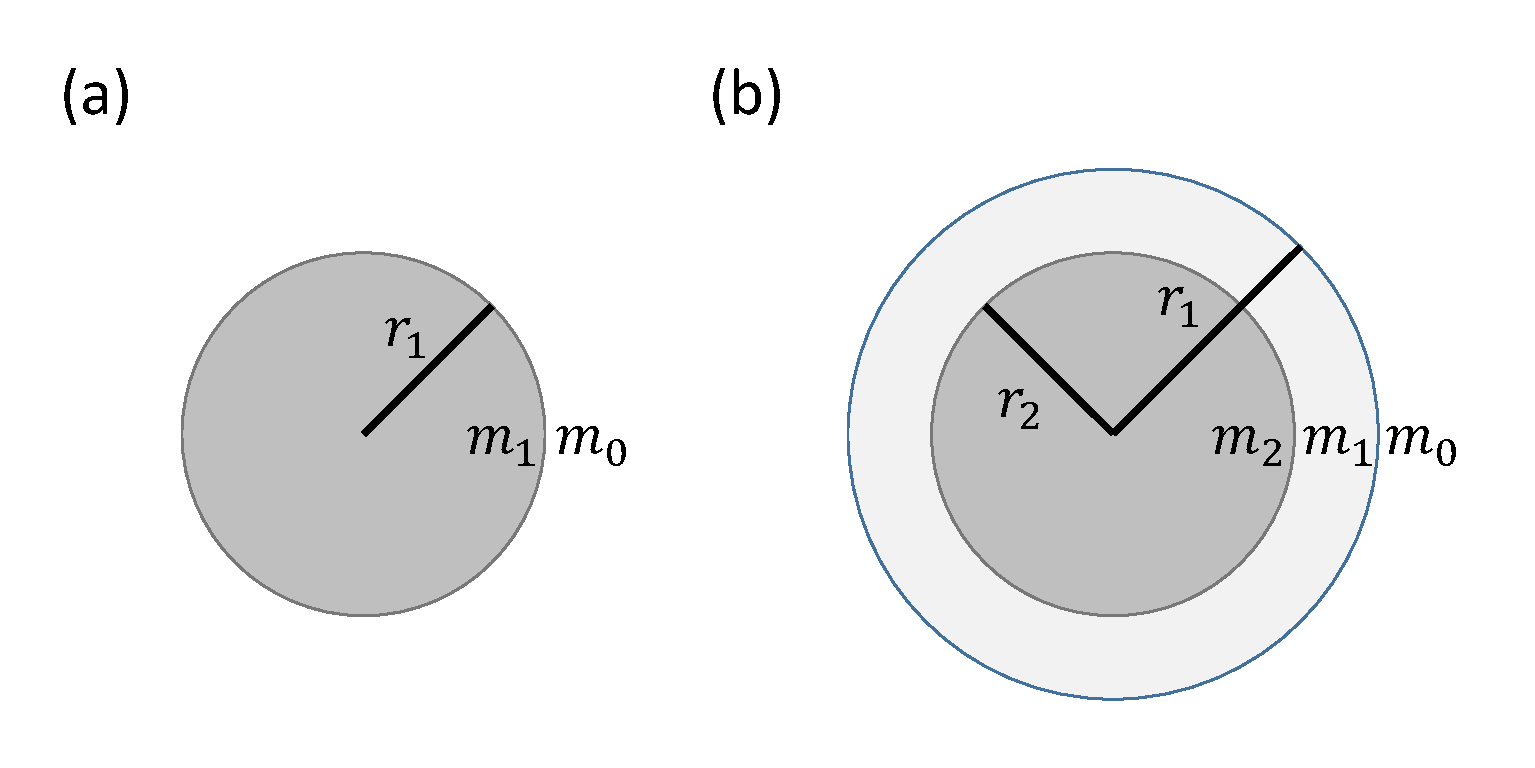
\includegraphics[width=1\textwidth]{Figures/BC.pdf}
    \caption{The structures of (a) single sphere and (b) core/shell sphere. $r_1$ represents the radius of the outer boundary, and $r_2$ represents the radius of the inner boundary (for the core/shell sphere).
    The dielectric function in each region is idealized to be homogeneous, i.e., independent of position.}
    \label{illustration}
    \end{center}
\end{figure*}
\noindent
In this subsection, we focus on the electric fields in the two systems, (a) single sphere and (b) core/shell sphere, as shown in Fig.~\ref{illustration}, in order to solve the dyadic Green's functions, $\tensorg_\mathrm{sour}^{(00)}(\mathbf{r,r'},\omega)$, $\tensorg_\mathrm{scat}^{(00)}(\mathbf{r,r'},\omega)$, and $\tensorg^{(10)}(\mathbf{r,r'},\omega)$.
As mentioned in Eq.~(\ref{Eq:InhomoPDEE}), we aim to solve the inhomogeneous vector differential equation,
\begin{align}
    %\label{Eq:InhomoPDEE}
    \nonumber
    &\left[\frac{\omega^2\epsilon_{\textrm{r},i}(\omega)}{c^2}-\nabla\times\nabla\times\right]\eme^{(i)}(\br,\omega)
    = -\frac{\omega^2}{\epsilon_0c^2}\sum_j\emp_\textrm{D}^{(j)}(\br,\omega).
\end{align}
According to the systems illustrated in Fig.~\ref{illustration}, the dielectric function of the two systems are shown in the following table.
In addition, the polarization $\emp_\mathrm{D}^{(j)}(\mathbf{r},\omega)$ is expressed as
\begin{align}
    \nonumber
    \sum_j\emp_\textrm{D}^{(j)}(\br,\omega) \rightarrow \emp_\textrm{D}^{(0)}(\br,\omega)=\vb{p}_\textrm{D}(\omega)\delta(\br-\br_\mathrm{D}).
\end{align}
\begin{table}[t]
    \renewcommand*{\arraystretch}{1.2}
    \begin{tabularx}{1\linewidth}{@{}m{2cm}<{\centering} *1{@{}m{0.2cm}@{}} *1{>{\arraybackslash}X}@{} *1{@{}>{\arraybackslash}r} *1{m{0.4cm}} *1{>{\arraybackslash}X} *1{@{}>{\arraybackslash}r}}%{lll}
        \hline\hline
         && \multicolumn{2}{c}{Single Sphere} &&  \multicolumn{2}{c}{Core/Shell Sphere} \\ \cline{1-7}%\cline{6-7}
        \multirow{3}{*}{$\epsilon_\mathrm{r}(\br,\omega)$} 
         && $\epsilon_\mathrm{r,0}(\omega)=1$  & $r>r_1$   && $\epsilon_\mathrm{r,0}(\omega)=1$ & $r>r_1$\\     %\cline{3-4}\cline{6-7}
         && $\epsilon_\mathrm{r,1}(\omega)$    & $r_1>r>0$ && $\epsilon_\mathrm{r,1}(\omega)$   & $r_1>r>r_2$\\ %\cline{3-4}\cline{6-7}
         && N/A                                & N/A       && $\epsilon_\mathrm{r,2}(\omega)$   & $r_2>r>0$\\   \hline\hline
    \end{tabularx}
    \caption{Dielectric function of the two systems. Note that $\epsilon_\mathrm{r}(\br,\omega)$ is piecewise-homogeneous.}
\end{table}

%\begin{align}
%    \begin{split}
%    \epsilon_{\mathrm{r,sin}}(\br,\omega) = 
%        \begin{cases}
%            \epsilon_{\mathrm{r},0}(\omega)=1, & r_1<r \\
%            \epsilon_{\mathrm{r},1}(\omega), & 0<r < r_1
%        \end{cases}
%    \end{split}\quad
%    \begin{split}
%    \epsilon_{\mathrm{r,c/s}}(\br,\omega) = 
%        \begin{cases}
%            \epsilon_{\mathrm{r},0}(\omega)=1, & r_1 < r\\
%            \epsilon_{\mathrm{r},1}(\omega), & r_2 < r < r_1\\
%            \epsilon_{\mathrm{r},2}(\omega), & 0 < r < r_2
%        \end{cases}
%    \end{split}.
%\end{align}
\noindent
In Eqs.~(\ref{Eq:EdipoleExpand}) and~(\ref{Eq:EdipoleExpandcoeff}), the electric point dipole are expanded to vector spherical functions.
The next procedure is solving the scattering process via considering the electromagnetic boundary condition.
In electrodynamics, the electric and magnetic field obey the four conditions for each boundary:
\begin{subequations}
    \begin{align}
        \label{boundE}
        \mathbf{n}_{i} \times \left[ \mathbf{E}^{(i)}(\mathbf{r}_{i},\omega) - \mathbf{E}^{(i-1)}(\mathbf{r}_{i},\omega)\right] &= 0,\\
        \label{boundD}
        \mathbf{n}_{i} \cdot \left[ \mathbf{D}^{(i)}(\mathbf{r}_{i},\omega) - \mathbf{D}^{(i-1)}(\mathbf{r}_{i},\omega)\right] &= \sigma_s,\\
        \label{boundB}
        \mathbf{n}_{i} \cdot \left[ \mathbf{B}^{(i)}(\mathbf{r}_{i},\omega) - \mathbf{B}^{(i-1)}(\mathbf{r}_{i},\omega)\right] &= 0,\\
        \label{boundH}
        \mathbf{n}_{i} \times \left[ \mathbf{H}^{(i)}(\mathbf{r}_{i},\omega) - \mathbf{H}^{(i-1)}(\mathbf{r}_{i},\omega)\right] &= \mathbf{j}_s
        .%,\quad i=j+1,\quad j = 0,~1,~2...
    \end{align}
    \label{Eq:EBC}%
\end{subequations}
where $i=1$ for the single sphere system and $i=1,~2$ for the core/shell system.
$\mathbf{n}_{l}$ is the normal vector of the boundary surface between $l^\textrm{th}$ region and $(l-1)^\textrm{th}$ region.
$\sigma_\textrm{s}$ and $\mathbf{j}_\textrm{s}$ denote the surface charge and the surface current density, respectively.
$\mathbf{r}_{l}$ describes the position vector of boundary, and $\omega$ represents the angular frequency.
Note that the bounded surface charge and bounded surface current density are equal to zero, in our cases.
In the following two subsections, we will individually discuss the two cases.
Specifically, the electric field is projected on the vector spherical functions and solve the corresponding coefficients by Eqs.~(\ref{boundE})~to~(\ref{boundH}).
Additional details can be found in the textbook.\cite{bohren2008absorption}
\subsubsectiontoc{Single Sphere}
For a single sphere illustrated in Figure~\ref{illustration}a, the electric field for each region is written as
\begin{subequations}
    \begin{align}
        \label{sphereE0}
        &\mathbf{E}_{\mathstrut}^{(0)}(\mathbf{r},\omega) = \mathbf{E}_{\textrm{sour}\mathstrut}^{(0)}(\mathbf{r},\omega) + \mathbf{E}_{\textrm{scat}\mathstrut}^{(0)}(\mathbf{r},\omega),\\
        \label{sphereE1}
        &\mathbf{E}_{\mathstrut}^{(1)}(\mathbf{r},\omega) = \mathbf{E}_{\mathstrut\textrm{core}}^{(1)}(\mathbf{r},\omega).
    \end{align}
\end{subequations}
%We give a superscript label on the electric fields corresponding to the defined regions.
In the zeroth region, the total electric field is separated into two parts, the source part $\mathbf{E}_{\textrm{sour}\mathstrut}^{(0)}(\mathbf{r},\omega)$ and the scattering part $\mathbf{E}_{\textrm{scat}\mathstrut}^{(0)}(\mathbf{r},\omega)$, in order to distinguish incident processes and scattering processes.
In the first region, $\mathbf{E}_{\mathstrut\textrm{core}}^{(1)}(\mathbf{r},\omega)$ describes the transmitted electric field in the core. 
For the electric fields, they can be projected on the two spherical vector  functions, $\norF{N}_{nm}^{(j)}(k_ir,\theta,\phi)$ and $\norF{M}_{nm}^{(j)}(k_ir,\theta,\phi)$,
\begin{subequations}
    \begin{align}
            \mathbf{E}_{\textrm{sour}\mathstrut}^{(0)}(\mathbf{r},\omega)
            &= \sum_{nm} \left[r_{nm}\norF{N}_{nm}^{(\RomanIII)}(k_0r,\theta,\phi) + s_{nm}\norF{M}_{nm}^{(\RomanIII)}(k_0r,\theta,\phi)\right], \hspace{2.8 cm} r>r_\mathrm{D}\\
            \mathbf{E}_{\textrm{sour}\mathstrut}^{(0)}(\mathbf{r},\omega)
            &= \sum_{nm} \left[p_{nm}\norF{N}_{nm}^{(\RomanI)}(k_0r,\theta,\phi) + q_{nm}\norF{M}_{nm}^{(\RomanI)}(k_0r,\theta,\phi)\right], \hspace{1.9 cm} r_1<r<r_\mathrm{D}\\
            \mathbf{E}_{\textrm{scat}\mathstrut}^{(0)}(\mathbf{r},\omega)
            &= \sum_{nm} \left[p_{nm}\alpha_n^{(0)}\norF{N}_{nm}^{(\RomanIII)}(k_0r,\theta,\phi) + q_{nm}\beta_n^{(0)}\norF{M}_{nm}^{(\RomanIII)}(k_0r,\theta,\phi)\right], \hspace{1.5 cm} r>r_1\\
            \mathbf{E}_{\textrm{core}\mathstrut}^{(1)}(\mathbf{r},\omega)
            &= \sum_{nm} \left[p_{nm}\delta_n^{(1)}\norF{N}_{nm}^{(\RomanI)}(k_1r,\theta,\phi) + q_{nm}\gamma_n^{(1)}\norF{M}_{nm}^{(\RomanI)}(k_1r,\theta,\phi)\right], \qquad 0<r<r_1.
    \end{align}
    \label{Eq:ESexpand}
\end{subequations}
where the summation runs from $n = 1$ to $\infty$ and from $m = -n$ to $n$.
To write down Eq.~(\ref{Eq:ESexpand}), the following four things should be explained.
First, we do not consider $\norF{L}_{nm}^{(j)}(k_ir,\theta,\phi)$ since the coefficients of the source (electric point dipole) to $\norF{L}_{nm}^{(j)}(k_ir,\theta,\phi)$ are zero.
Also note that the superscript of spherical vector functions [$\norF{N}_{nm}^{(j)}(k_ir,\theta,\phi)$ and $\norF{M}_{nm}^{(j)}(k_ir,\theta,\phi)$] indicates the type of spherical Bessel function used in the radial part rather than the region of piecewise dielectric environment.
Specifically, $j=\NRomanI$ indicates the use of the spherical Bessel functions and $j=\NRomanIII$ indicates the use of the spherical Hankel functions of the first kind.
Second, for a second-order differential equation, there are two independent solutions for the radial function.
We use spherical Bessel functions and spherical Hankel functions of the first kind as the two linear independent solutions to describe $\mathbf{E}_{\mathstrut}^{(0)}(\mathbf{r},\omega)$.
However, we only use spherical Bessel functions to describe $\mathbf{E}_{\mathstrut}^{(1)}(\mathbf{r},\omega)$ because spherical Hankel functions of the first kind diverged at zero and give nonphysical results.
Third, $\alpha_n^{(0)}$, $\beta_n^{(0)}$, $\gamma_n^{(1)}$, and $\delta_n^{(1)}$ are the Mie coefficients of an single sphere.
Here, $\alpha_n^{(0)}$ and $\beta_n^{(0)}$ can be interpreted as the reflective coefficients of TM fields and TE fields respectively; $\gamma_n^{(1)}$ and $\delta_n^{(1)}$ can be interpreted as the transmission coefficients TE fields and TM fields respectively.
Fourth, the Mie coefficients are only depend on $n$ due to the electromagnetic boundary condition in Eq.~(\ref{Eq:EBC}).
Comparing the vector spherical functions of the two regions, the only different variable is $k_ir$, which only influences on radial functions.
Therefore, Mie coefficients only associated with $n$.
Additionally, the magnetic fields are deduced by the relation: $i\omega\mu_0\mathbf{H}^{(i)}(\mathbf{r}_{i},\omega) = \nabla\times\mathbf{E}^{(i)}(\mathbf{r}_{i},\omega)$.
By considering Eqs.~(\ref{boundE})~-~(\ref{boundH}) at $r_i=r_1$, we get the four equations,
\begin{align}
    %&m_0\delta_{n}\psi_n'(m_1\rho_1) = 
    %m_1\psi_n'(m_0\rho_1) + m_1\alpha_n\xi_n'(m_0\rho_1)\\
    %&\gamma_{n}\psi_n'(m_1\rho_1) = 
    %\psi_n'(m_0\rho_1) + \beta_n\xi_n'(m_0\rho_1)\\
    %&\gamma_{n}\psi_n(m_1\rho_1) = 
    %\psi_n(m_0\rho_1) + \beta_n\xi_n(m_0\rho_1)\\
    %&m_1\delta_{n}\psi_n(m_1\rho_1) = 
    %m_0\psi_n(m_0\rho_1) + m_0\alpha_n\xi_n(m_0\rho_1)\\
    %\left\{
    \begin{array}{rlrlr}
    \nr_0\psi_n'(\nr_1\rho_1)\delta_n^{(1)} &=& 
    \nr_1\xi_n'(\nr_0\rho_1)\alpha_n^{(0)} &+& \nr_1\psi_n'(\nr_0\rho_1)\\
    \psi_n(\nr_1\rho_1)\delta_n^{(1)} &=& 
    \xi_n(\nr_0\rho_1)\alpha_n^{(0)} &+& \psi_n(\nr_0\rho_1)\\
    \nr_0\psi_n(\nr_1\rho_1)\gamma_n^{(1)} &=& 
    \nr_1\xi_n(\nr_0\rho_1)\beta_n^{(0)} &+& \nr_1\psi_n(\nr_0\rho_1)\\
    \psi_n'(\nr_1\rho_1)\gamma_n^{(1)} &=& 
    \xi_n'(\nr_0\rho_1)\beta_n^{(0)} &+& \psi_n'(\nr_0\rho_1)
    \end{array},
    %\right.
\end{align}
where $\xi_n(\nr_0\rho_1)=\nr_0\rho_1\cdot h_n^{(1)}(\nr_0\rho_1)$ is the $n$-th order of Riccati-Hankel functions of the first kind and $\rho_1\equiv k_0r_1$.
Recall that $k_i=\nr_ik_0$ and $\nr_i$ is the complex refractive index of the $i$-th region.
Although $\nr_0=1$ in the zeroth region, we still use $\nr_0$ in order to keep the symmetry of equations.
Solving the linear equations, we get the analytical expression of Mie coefficients,
\begin{subequations}
    \begin{align}
        \alpha_n^{(0)} &=-
        \frac{\nr_1\psi_n'(\nr_0\rho_1)\psi_n(\nr_1\rho_1)-\nr_0\psi_n(\nr_0\rho_1)\psi_n'(\nr_1\rho_1)}
        {\nr_1\xi_n'(\nr_0\rho_1)\psi_n(\nr_1\rho_1)-\nr_0\xi_n(\nr_0\rho_1)\psi_n'(\nr_1\rho_1)},\\
        \beta_n^{(0)} &=-
        \frac{\nr_0\psi_n'(\nr_0\rho_1)\psi_n(\nr_1\rho_1)-\nr_1\psi_n(\nr_0\rho_1)\psi_n'(\nr_1\rho_1)}
        {\nr_0\xi_n'(\nr_0\rho_1)\psi_n(\nr_1\rho_1)-\nr_1\xi_n(\nr_0\rho_1)\psi_n'(\nr_1\rho_1)},\\
        \gamma_n^{(1)} &=
        \frac{\nr_1\xi_n'(\nr_0\rho_1)\psi_n(\nr_0\rho_1)-\nr_1\xi_n(\nr_0\rho_1)\psi_n'(\nr_0\rho_1)}
        {\nr_0\xi_n'(\nr_0\rho_1)\psi_n(\nr_1\rho_1)-\nr_1\xi_n(\nr_0\rho_1)\psi_n'(\nr_1\rho_1)},\\
        \delta_n^{(1)} &=
        \frac{\nr_1\xi_n'(\nr_0\rho_1)\psi_n(\nr_0\rho_1)-\nr_1\xi_n(\nr_0\rho_1)\psi_n'(\nr_0\rho_1)}
        {\nr_1\xi_n'(\nr_0\rho_1)\psi_n(\nr_1\rho_1)-\nr_0\xi_n(\nr_0\rho_1)\psi_n'(\nr_1\rho_1)}.
    \end{align}
    \label{single}%
\end{subequations}
Applying Eq.~(\ref{single}) to Eq.~(\ref{Eq:ESexpand}), we are able to calculate the electric fields for each region now.
Furthermore, because the electric fields are equivalent to the Green's functions, we can also obtain the explicit expression of the dyadic Green's functions by the Mie coefficients,
\begin{align}
    \tensorg^{(00)}(\mathbf{r,r'},\omega)&=
    \tensorg_\mathrm{sour}^{(00)}(\mathbf{r,r'},\omega)+
    \tensorg_\mathrm{scat}^{(00)}(\mathbf{r,r'},\omega)\\
    \nonumber
    \tensorg^{(10)}(\mathbf{r,r'},\omega)&=
    ik_0 \sum_{nm}(-1)^m
    \left[\gamma_n^{(1)}\norF{M}_{\mathstrut{nm}}^{(\RomanI)}(k_1r,\theta,\phi)
    \otimes\norF{M}_{n(-m)}^{(\RomanIII)}(k_0r',\theta',\phi')\right.\\
    &\hspace{2.85 cm}
    \left.+\delta_n^{(1)}\norF{N}_{\mathstrut{nm}}^{(\RomanI)}(k_1r,\theta,\phi)\otimes
    \norF{N}_{n(-m)}^{(\RomanIII)}(k_0r',\theta',\phi')\right],
\end{align}
where $\tensorg_\mathrm{sour}^{(00)}(\mathbf{r,r'},\omega)$ and $\tensorg_\mathrm{scat}^{(00)}(\mathbf{r,r'},\omega)$ are
\begin{align}
    \label{G00sour}
    \overline{\overline{\mathbf{G}}}_\mathrm{sour}^{(00)}(\mathbf{r,r'},\omega)=
    \begin{cases}
        \displaystyle
        ik_0 \sum_{nm}(-1)^m\left[\norF{M}_{\mathstrut{nm}}^{(\RomanI)}(k_0r,\theta,\phi)
        \otimes\norF{M}_{n(-m)}^{(\RomanIII)}(k_0r',\theta',\phi')\right.\\
        \hspace{2.34cm}\left.+\norF{N}_{\mathstrut{nm}}^{(\RomanI)}(k_0r,\theta,\phi)
        \otimes\norF{N}_{n(-m)}^{(\RomanIII)}(k_0r',\theta',\phi')\right], & r < r'\\
        \displaystyle
        ik_0 \sum_{nm}(-1)^m\left[\norF{M}_{\mathstrut{nm}}^{(\RomanIII)}(k_0r,\theta,\phi)
        \otimes\norF{M}_{n(-m)}^{(\RomanI)}(k_0r',\theta',\phi')\right.\\
        \hspace{2.34cm}\left.+\norF{N}_{\mathstrut{nm}}^{(\RomanIII)}(k_0r,\theta,\phi)
        \otimes\norF{N}_{n(-m)}^{(\RomanI)}(k_0r',\theta',\phi')\right], & r > r'
    \end{cases},%
\end{align}
and 
\begin{align}
    \nonumber
    \overline{\overline{\mathbf{G}}}_\mathrm{scat}^{(00)}(\mathbf{r,r'},\omega)=
    ik_0 \sum_{nm}(-1)^m
    &\left[\beta_n^{(0)}\norF{M}_{\mathstrut{nm}}^{(\RomanIII)}(k_0r,\theta,\phi)
    \otimes\norF{M}_{n(-m)}^{(\RomanIII)}(k_0r',\theta',\phi')\right.\\
    &\left.+\alpha_n^{(0)}\norF{N}_{\mathstrut{nm}}^{(\RomanIII)}(k_0r,\theta,\phi)\otimes\norF{N}_{n(-m)}^{(\RomanIII)}(k_0r',\theta',\phi')\right],\hspace{1.42 cm}
    \label{G00scat}
\end{align}
respectively.
\newpage
\subsubsectiontoc{Core/Shell Sphere}
%\addcontentsline{toc}{subsubsection}{Core/Shell Sphere}
For a core/shell sphere system illustrated in Figure~\ref{illustration}b, we need to deal with two boundary constraints. Hence, there are three regions for the electric field:
\begin{subequations}
    \begin{align}
        \label{cssphereE0}
        &\mathbf{E}_{\mathstrut}^{(0)}(\mathbf{r},\omega) = \mathbf{E}_{\textrm{sour}\mathstrut}^{(0)}(\mathbf{r},\omega) + \mathbf{E}_{\textrm{scat}\mathstrut}^{(0)}(\mathbf{r},\omega),\\
        \label{cssphereE1}
        &\mathbf{E}_{\mathstrut}^{(1)}(\mathbf{r},\omega) = \mathbf{E}_{\mathstrut\textrm{shell}}^{(1)}(\mathbf{r},\omega),\\
        \label{cssphereE2}
        &\mathbf{E}_{\mathstrut}^{(2)}(\mathbf{r},\omega) =     \mathbf{E}_{\mathstrut\textrm{core}}^{(2)}(\mathbf{r},\omega).
    \end{align}%
\end{subequations}
Using the same strategy as explained in the previous subsection, we can express the electric fields for each region by
\begin{subequations}
    \begin{align}
            \mathbf{E}_{\textrm{sour}\mathstrut}^{(0)}(\mathbf{r},\omega)
            &= \sum_{nm} \left[r_{nm}\norF{N}_{nm}^{(\RomanIII)}(k_0r,\theta,\phi) + s_{nm}\norF{M}_{nm}^{(\RomanIII)}(k_0r,\theta,\phi)\right], \hspace{2.95 cm} r>r_\mathrm{D}\\
            \mathbf{E}_{\textrm{sour}\mathstrut}^{(0)}(\mathbf{r},\omega)
            &= \sum_{nm} \left[p_{nm}\norF{N}_{nm}^{(\RomanI)}(k_0r,\theta,\phi) + q_{nm}\norF{M}_{nm}^{(\RomanI)}(k_0r,\theta,\phi)\right], \hspace{2.05 cm} r_1<r<r_\mathrm{D}\\
            \mathbf{E}_{\textrm{scat}\mathstrut}^{(0)}(\mathbf{r},\omega)
            &= \sum_{nm} \left[p_{nm}\alpha_n^{(0)}\mathbf{N}_{nm}^{(\RomanIII)}(k_0r,\theta,\phi) + q_{nm}\beta_n^{(0)}\mathbf{M}_{nm}^{(\RomanIII)}(k_0r,\theta,\phi)\right], \hspace{1.69 cm} r>r_1\\
            \nonumber
            \mathbf{E}_{\textrm{shell}\mathstrut}^{(1)}(\mathbf{r},\omega)
            &= \sum_{nm} \left[p_{nm}\alpha_n^{(1)}\mathbf{N}_{nm}^{(\RomanIII)}(k_1r,\theta,\phi) + q_{nm}\beta_n^{(1)}\mathbf{M}_{nm}^{(\RomanIII)}(k_1r,\theta,\phi)\right.\\
            &\hspace{.9 cm}+ \left.p_{nm}\delta_n^{(1)}\mathbf{N}_{nm}^{(\RomanI)}(k_1r,\theta,\phi) + q_{nm}\gamma_n^{(1)}\mathbf{M}_{nm}^{(\RomanI)}(k_1r,\theta,\phi)\right], \qquad r_2<r<r_1\\
            \mathbf{E}_{\textrm{core}\mathstrut}^{(2)}(\mathbf{r},\omega)
            &= \sum_{nm} \left[p_{nm}\delta_n^{(2)}\mathbf{N}_{nm}^{(\RomanI)}(k_2r,\theta,\phi) + q_{nm}\gamma_n^{(2)}\mathbf{M}_{nm}^{(\RomanI)}(k_2r,\theta,\phi)\right], \hspace{1.0 cm} 0<r<r_2,
    \end{align}
    \label{Eq:ECSexpand}%
\end{subequations}
Especially, in the location of the shell, we use both Bessel-type functions and Hankel-type functions to describe the electric field because both of them are not suppressed by boundary conditions.
In the same way, the magnetic fields are defined according to the relation, $i\omega\mu_0\mathbf{H}^{(i)}(\mathbf{r}_{i},\omega) = \nabla\times\mathbf{E}^{(i)}(\mathbf{r}_{i},\omega)$.
By considering the boundary conditions in Eqs.~(\ref{boundE})~-~(\ref{boundH}) at $r_i=r_1~\mathrm{and}~r_2$ , we obtain the eight equations,
\begin{align}
    &\begin{array}{rlrlrlr}
     & & \nr_1\psi_n'(\nr_2\rho_2)\delta_n^{(2)} &=& 
    \nr_2\xi_n'(\nr_1\rho_2)\alpha_n^{(1)} & + & \nr_2\psi_n'(\nr_1\rho_2)\delta_n^{(1)}\\
     & & \psi_n(\nr_2\rho_2)\delta_n^{(2)} &=& 
    \xi_n(\nr_1\rho_2)\alpha_n^{(1)} &+& \psi_n(\nr_1\rho_2)\delta_n^{(1)}\\
     & & \nr_1\psi_n(\nr_2\rho_2)\gamma_n^{(2)} &=& 
    \nr_2\xi_n(\nr_1\rho_2)\beta_n^{(1)} &+& \nr_2\psi_n(\nr_1\rho_2)\gamma_n^{(1)}\\
     & & \psi_n'(\nr_2\rho_2)\gamma_n^{(2)} &=& 
    \xi_n'(\nr_1\rho_2)\beta_n^{(1)} &+& \psi_n'(\nr_1\rho_2)\gamma_n^{(1)}\\
    %\end{array}\\
    %&\begin{array}{rlrlrlr}
    \nr_0\xi_n'(\nr_1\rho_1)\alpha_n^{(1)} &+& \nr_0\psi_n'(\nr_1\rho_1)\delta_n^{(1)} &=& 
    \nr_1\xi_n'(\nr_0\rho_1)\alpha_n^{(0)} &+& \nr_1\psi_n'(\nr_0\rho_1)\hphantom{\delta_n^{(1)}}\\
    \xi_n(\nr_1\rho_1)\alpha_n^{(1)} &+& \psi_n(\nr_1\rho_1)\delta_n^{(1)} &=& 
    \xi_n(\nr_0\rho_1)\alpha_n^{(0)} &+& \psi_n(\nr_0\rho_1)\hphantom{\delta_n^{(1)}}\\
    \nr_0\xi_n(\nr_1\rho_1)\beta_n^{(1)} &+& \nr_0\psi_n(\nr_1\rho_1)\gamma_n^{(1)} &=& 
    \nr_1\xi_n(\nr_0\rho_1)\beta_n^{(0)} &+& \nr_1\psi_n(\nr_0\rho_1)\hphantom{\delta_n^{(1)}}\\
    \xi_n'(\nr_1\rho_1)\beta_n^{(1)} &+& \psi_n'(\nr_1\rho_1)\gamma_n^{(1)} &=& 
    \xi_n'(\nr_0\rho_1)\beta_n^{(0)} &+& \psi_n'(\nr_0\rho_1)\hphantom{\delta_n^{(1)}}
    \end{array},
\end{align}
where $\rho_2=k_0r_2$ and $\rho_1=k_0r_1$.
Note that the eight equation can be separated to two set of simultaneous equations which is guaranteed by the orthogonality of $\norF{M}_{nm}^{(j)}(k_ir,\theta,\phi)$ and $\norF{N}_{nm}^{(j)}(k_ir,\theta,\phi)$.
Furthermore, for the concern of numerical stability, we substitute the derivatives of Riccati-Bessel (-Hankel) functions for logarithmic derivatives,
\begin{subequations}
    \begin{align}
        &\mathcal{D}\psi_n(z) = \frac{\mathrm{d}}{\mathrm{d}z}\ln{\psi_n(z)} = \frac{\psi_n'(z)}{\psi_n(z)},\\
        &\mathcal{D}\xi_n(z) = \frac{\mathrm{d}}{\mathrm{d}z}\ln{\xi_n(z)} = \frac{\xi_n'(z)}{\xi_n(z)}.
    \end{align}%
\end{subequations}
It has been mentioned that the logarithmic derivative of Riccati-Bessel (-Hankel) function is numerically more stable than the derivative of Riccati-Bessel (-Hankel) function\cite{jia2016calculation}.
Solving the above equations, the Mie scattering coefficients turn out to:
\begin{subequations}
    \begin{align}
        \label{coreshell_alpha}
        \alpha_n^{(0)} &=
        \frac{\mathcal{A}_1-\mathcal{A}}{\mathcal{A}_2-\mathcal{A}}\cdot
        \frac{\nr_0\mathcal{D}\psi_n(\nr_1\rho_1)-\nr_1\mathcal{D}\psi_n(\nr_0\rho_1)}
        {\nr_1\mathcal{D}\xi_n(\nr_0\rho_1)-\nr_0\mathcal{D}\psi_n(\nr_1\rho_1)}\cdot
        \frac{\psi_n(\nr_0\rho_1)}{\xi_n(\nr_0\rho_1)},\\
        \label{coreshell_beta}
        \beta_n^{(0)} &=
        \frac{\mathcal{B}_1-\mathcal{B}}{\mathcal{B}_2-\mathcal{B}}\cdot
        \frac{\nr_0\mathcal{D}\psi_n(\nr_0\rho_1)-\nr_1\mathcal{D}\psi_n(\nr_1\rho_1)}
        {\nr_1\mathcal{D}\psi_n(\nr_1\rho_1)-\nr_0\mathcal{D}\xi_n(\nr_0\rho_1)}\cdot
        \frac{\psi_n(\nr_0\rho_1)}{\xi_n(\nr_0\rho_1)},
    \end{align}
    \label{coreshell}
\end{subequations}
where
\begin{subequations}
    \begin{align}
        \mathcal{A} =& \frac{\nr_2\mathcal{D}\xi_n(\nr_1\rho_2)-\nr_1\mathcal{D}\psi_n(\nr_2\rho_2)}
        {\nr_1\mathcal{D}\psi_n(\nr_2\rho_2)-\nr_2\mathcal{D}\psi_n(\nr_1\rho_2)}
        \cdot\frac{\xi_n(\nr_1\rho_2)}{\psi_n(\nr_1\rho_2)},\\
        \mathcal{B} =& \frac{\nr_2\mathcal{D}\psi_n(\nr_2\rho_2)-\nr_1\mathcal{D}\xi_n(\nr_1\rho_2)}
        {\nr_1\mathcal{D}\psi_n(\nr_1\rho_2)-\nr_2\mathcal{D}\psi_n(\nr_2\rho_2)}
        \cdot\frac{\xi_n(\nr_1\rho_2)}{\psi_n(\nr_1\rho_2)},\\
        \mathcal{A}_1 = & \frac{\nr_1\mathcal{D}\psi_n(\nr_0\rho_1)-\nr_0\mathcal{D}\xi_n(\nr_1\rho_1)}
        {\nr_0\mathcal{D}\psi_n(\nr_1\rho_1)-\nr_1\mathcal{D}\psi_n(\nr_0\rho_1)}
        \cdot\frac{\xi_n(\nr_1\rho_1)}{\psi_n(\nr_1\rho_1)},\\
        \mathcal{A}_2 = & \frac{\nr_0\mathcal{D}\xi_n(\nr_1\rho_1)-\nr_1\mathcal{D}\xi_n(\nr_0\rho_1)}
        {\nr_1\mathcal{D}\xi_n(\nr_0\rho_1)-\nr_0\mathcal{D}\psi_n(\nr_1\rho_1)}
        \cdot\frac{\xi_n(\nr_1\rho_1)}{\psi_n(\nr_1\rho_1)},\\
        \mathcal{B}_1 =& \frac{\nr_1\mathcal{D}\xi_n(\nr_1\rho_1)-\nr_0\mathcal{D}\psi_n(\nr_0\rho_1)}
        {\nr_0\mathcal{D}\psi_n(\nr_0\rho_1)-\nr_1\mathcal{D}\psi_n(\nr_1\rho_1)}
        \cdot\frac{\xi_n(\nr_1\rho_1)}{\psi_n(\nr_1\rho_1)},\\
        \mathcal{B}_2 =& \frac{\nr_0\mathcal{D}\xi_n(\nr_0\rho_1)-\nr_1\mathcal{D}\xi_n(\nr_1\rho_1)}
        {\nr_1\mathcal{D}\psi_n(\nr_1\rho_1)-\nr_0\mathcal{D}\xi_n(\nr_0\rho_1)}
        \cdot\frac{\xi_n(\nr_1\rho_1)}{\psi_n(\nr_1\rho_1)}.
    \end{align}    
\end{subequations}
The calculations of the logarithmic derivatives of Riccati-Bessel (Hankel) functions can be found in the previous study.\cite{jia2016calculation}
Using the same strategy described in the section on a single sphere, we would obtain the explicit expression of the dyadic Green's functions,
\begin{align}
    \tensorg^{(00)}(\mathbf{r,r'},\omega)&=
    \tensorg_\mathrm{sour}^{(00)}(\mathbf{r,r'},\omega)+
    \tensorg_\mathrm{scat}^{(00)}(\mathbf{r,r'},\omega)\\
    \nonumber
    \tensorg^{(10)}(\mathbf{r,r'},\omega)&=
    ik_0 \sum_{nm}(-1)^m
    \left[\beta_n^{(1)}\norF{M}_{\mathstrut{nm}}^{(\RomanIII)}(k_1r,\theta,\phi)
    \otimes\norF{M}_{n(-m)}^{(\RomanIII)}(k_0r',\theta',\phi')\right.\\
    &\hspace{2.85 cm}
    \left.+\alpha_n^{(1)}\norF{N}_{\mathstrut{nm}}^{(\RomanIII)}(k_1r,\theta,\phi)\otimes\norF{N}_{n(-m)}^{(\RomanIII)}(k_0r',\theta',\phi')\right.\\
    &\hspace{2.85 cm}
    \left.+\gamma_n^{(1)}\norF{M}_{\mathstrut{nm}}^{(\RomanI)}(k_1r,\theta,\phi)
    \otimes\norF{M}_{n(-m)}^{(\RomanIII)}(k_0r',\theta',\phi')\right.\\
    &\hspace{2.85 cm}
    \left.+\delta_n^{(1)}\norF{N}_{\mathstrut{nm}}^{(\RomanI)}(k_1r,\theta,\phi)\otimes
    \norF{N}_{n(-m)}^{(\RomanIII)}(k_0r',\theta',\phi')\right],\\
    \nonumber
    \tensorg^{(20)}(\mathbf{r,r'},\omega)&=
    ik_0 \sum_{nm}(-1)^m
    \left[\gamma_n^{(2)}\norF{M}_{\mathstrut{nm}}^{(\RomanI)}(k_1r,\theta,\phi)
    \otimes\norF{M}_{n(-m)}^{(\RomanIII)}(k_0r',\theta',\phi')\right.\\
    &\hspace{2.85 cm}
    \left.+\delta_n^{(2)}\norF{N}_{\mathstrut{nm}}^{(\RomanI)}(k_1r,\theta,\phi)\otimes
    \norF{N}_{n(-m)}^{(\RomanIII)}(k_0r',\theta',\phi')\right],
\end{align}
where $\tensorg_\mathrm{sour}^{(00)}(\mathbf{r,r'},\omega)$ and have the same form as described in Eqs.~(\ref{G00sour}) and (\ref{G00scat}); the only difference is the scattering coefficients, $\alpha_n^{(0)}$ and $\beta_n^{(0)}$.
\newpage
%\begin{blue}
\begin{comment}
\subsubsection{Spherical Cavity}
\addcontentsline{toc}{subsubsection}{Spherical Cavity}
For a spherical cavity system, it is similar to the case of core/shell sphere, but the dipole is located beneath the shell. Hence, the space is divided into three regions, and the electric field in each region becomes
\begin{subequations}
    \begin{align}
        \label{cavsphereE0}
        &\mathbf{E}_{\mathstrut}^{(0)}(\mathbf{r},\omega) =  \mathbf{E}_{\textrm{scat}\mathstrut}^{(0)}(\mathbf{r},\omega),\\
        \label{cavsphereE1}
        &\mathbf{E}_{\mathstrut}^{(1)}(\mathbf{r},\omega) = \mathbf{E}_{\mathstrut\textrm{shell}}^{(1)}(\mathbf{r},\omega),\\
        \label{cavsphereE2}
        &\mathbf{E}_{\mathstrut}^{(2)}(\mathbf{r},\omega) =
        \mathbf{E}_{\textrm{sour}\mathstrut}^{(2)}(\mathbf{r},\omega) +
        \mathbf{E}_{\mathstrut\textrm{refl}}^{(2)}(\mathbf{r},\omega).
    \end{align}
\end{subequations}
As explained in previous subsection, we write down the electric fields
\begin{subequations}
    \begin{align}
            \mathbf{E}_{\textrm{scat}\mathstrut}^{(0)}(\mathbf{r},\omega)
            &= \sum_{nm} \left[r_{nm}\alpha_n^{(0)}\mathbf{N}_{nm}^{(\RomanIII)}(k_0r,\theta,\phi) + s_{nm}\beta_n^{(0)}\mathbf{M}_{nm}^{(\RomanIII)}(k_0r,\theta,\phi)\right], \hspace{1.67 cm} r>r_1\\
            \nonumber
            \mathbf{E}_{\textrm{shell}\mathstrut}^{(1)}(\mathbf{r},\omega)
            &= \sum_{nm} \left[r_{nm}\alpha_n^{(1)}\mathbf{N}_{nm}^{(\RomanIII)}(k_1r,\theta,\phi) + s_{nm}\beta_n^{(1)}\mathbf{M}_{nm}^{(\RomanIII)}(k_1r,\theta,\phi)\right.\\
            &\hspace{.9 cm}+ \left.r_{nm}\delta_n^{(1)}\mathbf{N}_{nm}^{(\RomanI)}(k_1r,\theta,\phi) + s_{nm}\gamma_n^{(1)}\mathbf{M}_{nm}^{(\RomanI)}(k_1r,\theta,\phi)\right], \qquad r_2<r<r_1\\
            \mathbf{E}_{\textrm{sour}\mathstrut}^{(2)}(\mathbf{r},\omega)
            &= \sum_{nm} \left[r_{nm}\norF{N}_{nm}^{(\RomanIII)}(k_0r,\theta,\phi) + s_{nm}\norF{M}_{nm}^{(\RomanIII)}(k_0r,\theta,\phi)\right], \hspace{1.95 cm} r_\mathrm{D}<r<r_2\\
            \mathbf{E}_{\textrm{sour}\mathstrut}^{(2)}(\mathbf{r},\omega)
            &= \sum_{nm} \left[p_{nm}\norF{N}_{nm}^{(\RomanI)}(k_0r,\theta,\phi) + q_{nm}\norF{M}_{nm}^{(\RomanI)}(k_0r,\theta,\phi)\right], \hspace{2.2 cm} 0<r<r_\mathrm{D}\\
            \mathbf{E}_{\textrm{core}\mathstrut}^{(2)}(\mathbf{r},\omega)
            &= \sum_{nm} \left[r_{nm}\delta_n^{(2)}\mathbf{N}_{nm}^{(\RomanI)}(k_2r,\theta,\phi) + s_{nm}\gamma_n^{(2)}\mathbf{M}_{nm}^{(\RomanI)}(k_2r,\theta,\phi)\right], \hspace{1.05 cm} 0<r<r_2,
    \end{align}
\end{subequations}
and get eight linear equations:
\begin{align}
    &\begin{array}{rlrlrlr}
    \nr_1\xi_n'(\nr_2\rho_2)\hphantom{\alpha_n^{(1)}} &+& \nr_1\psi_n'(\nr_2\rho_2)\delta_n^{(2)} &=& 
    \nr_2\xi_n'(\nr_1\rho_2)\alpha_n^{(1)} &+& \nr_2\psi_n'(\nr_1\rho_2)\delta_n^{(1)}\\
    \xi_n(\nr_2\rho_2)\hphantom{\alpha_n^{(1)}} &+& \psi_n(\nr_2\rho_2)\delta_n^{(2)} &=& 
    \xi_n(\nr_1\rho_2)\alpha_n^{(1)} &+& \psi_n(\nr_1\rho_2)\delta_n^{(1)}\\
    \nr_1\xi_n(\nr_2\rho_2)\hphantom{\alpha_n^{(1)}} &+& \nr_1\psi_n(\nr_2\rho_2)\gamma_n^{(2)} &=& 
    \nr_2\xi_n(\nr_1\rho_2)\beta_n^{(1)} &+& \nr_2\psi_n(\nr_1\rho_2)\gamma_n^{(1)}\\
    \xi_n'(\nr_2\rho_2)\hphantom{\alpha_n^{(1)}} &+& \psi_n'(\nr_2\rho_2)\gamma_n^{(2)} &=& 
    \xi_n'(\nr_1\rho_2)\beta_n^{(1)} &+& \psi_n'(\nr_1\rho_2)\gamma_n^{(1)}\\
    %\end{array}\\
    %&\begin{array}{rlrlrlr}
    \nr_0\xi_n'(\nr_1\rho_1)\alpha_n^{(1)} &+& \nr_0\psi_n'(\nr_1\rho_1)\delta_n^{(1)} &=& 
    \nr_1\xi_n'(\nr_0\rho_1)\alpha_n^{(0)} & & \hphantom{\delta_n^{(1)}}\\
    \xi_n(\nr_1\rho_1)\alpha_n^{(1)} &+& \psi_n(\nr_1\rho_1)\delta_n^{(1)} &=& 
    \xi_n(\nr_0\rho_1)\alpha_n^{(0)} & & \hphantom{\delta_n^{(1)}}\\
    \nr_0\xi_n(\nr_1\rho_1)\beta_n^{(1)} &+& \nr_0\psi_n(\nr_1\rho_1)\gamma_n^{(1)} &=& 
    \nr_1\xi_n(\nr_0\rho_1)\beta_n^{(0)} & & \hphantom{\delta_n^{(1)}}\\
    \xi_n'(\nr_1\rho_1)\beta_n^{(1)} &+& \psi_n'(\nr_1\rho_1)\gamma_n^{(1)} &=& 
    \xi_n'(\nr_0\rho_1)\beta_n^{(0)} & & \hphantom{\delta_n^{(1)}}
    \end{array},
\end{align}
where $\rho_2=k_0r_2$ and $\rho_1=k_0r_1$.

For the concern of numerical stability, we should modify the equations. Here, we substitute the derivatives of Riccati-Bessel (Hankel) functions for logarithmic derivatives:
\begin{subequations}
    \begin{align}
        &\mathcal{D}\psi_n(x) = \frac{\mathrm{d}}{\mathrm{d}x}\ln{\psi_n(x)} = \frac{\psi_n'(x)}{\psi_n(x)},\\
        &\mathcal{D}\xi_n(x) = \frac{\mathrm{d}}{\mathrm{d}x}\ln{\xi_n(x)} = \frac{\xi_n'(x)}{\xi_n(x)}.
    \end{align}
\end{subequations}
Solving the above equations, the Mie scattering coefficients turn out to:
\begin{align}
    \label{cavity_alpha}
    \alpha_n \equiv \alpha_n^{(0)} &=
    \frac{\mathcal{A}_1-\mathcal{A}}{\mathcal{A}_2-\mathcal{A}}\cdot
    \frac{\nr_0\mathcal{D}\psi_n(\nr_1\rho_1)-\nr_1\mathcal{D}\psi_n(\nr_0\rho_1)}
    {\nr_1\mathcal{D}\xi_n(\nr_0\rho_1)-\nr_0\mathcal{D}\psi_n(\nr_1\rho_1)}\cdot
    \frac{\psi_n(\nr_0\rho_1)}{\xi_n(\nr_0\rho_1)},\\
    \label{cavity_beta}
    \beta_n \equiv \beta_n^{(0)} &=
    \frac{\mathcal{B}_1-\mathcal{B}}{\mathcal{B}_2-\mathcal{B}}\cdot
    \frac{\nr_0\mathcal{D}\psi_n(\nr_0\rho_1)-\nr_1\mathcal{D}\psi_n(\nr_1\rho_1)}
    {\nr_1\mathcal{D}\psi_n(\nr_1\rho_1)-\nr_0\mathcal{D}\xi_n(\nr_0\rho_1)}\cdot
    \frac{\psi_n(\nr_0\rho_1)}{\xi_n(\nr_0\rho_1)},
\end{align}
where
\begin{subequations}
    \begin{align}
        \mathcal{A} =& \frac{\nr_2\mathcal{D}\xi_n(\nr_1\rho_2)-\nr_1\mathcal{D}\psi_n(\nr_2\rho_2)}
        {\nr_1\mathcal{D}\psi_n(\nr_2\rho_2)-\nr_2\mathcal{D}\psi_n(\nr_1\rho_2)}
        \cdot\frac{\xi_n(\nr_1\rho_2)}{\psi_n(\nr_1\rho_2)},\\
        \mathcal{B} =& \frac{\nr_2\mathcal{D}\psi_n(\nr_2\rho_2)-\nr_1\mathcal{D}\xi_n(\nr_1\rho_2)}
        {\nr_1\mathcal{D}\psi_n(\nr_1\rho_2)-\nr_2\mathcal{D}\psi_n(\nr_2\rho_2)}
        \cdot\frac{\xi_n(\nr_1\rho_2)}{\psi_n(\nr_1\rho_2)},\\
        \mathcal{A}_1 = & \frac{\nr_1\mathcal{D}\psi_n(\nr_0\rho_1)-\nr_0\mathcal{D}\xi_n(\nr_1\rho_1)}
        {\nr_0\mathcal{D}\psi_n(\nr_1\rho_1)-\nr_1\mathcal{D}\psi_n(\nr_0\rho_1)}
        \cdot\frac{\xi_n(\nr_1\rho_1)}{\psi_n(\nr_1\rho_1)},\\
        \mathcal{A}_2 = & \frac{\nr_0\mathcal{D}\xi_n(\nr_1\rho_1)-\nr_1\mathcal{D}\xi_n(\nr_0\rho_1)}
        {\nr_1\mathcal{D}\xi_n(\nr_0\rho_1)-\nr_0\mathcal{D}\psi_n(\nr_1\rho_1)}
        \cdot\frac{\xi_n(\nr_1\rho_1)}{\psi_n(\nr_1\rho_1)},\\
        \mathcal{B}_1 =& \frac{\nr_1\mathcal{D}\xi_n(\nr_1\rho_1)-\nr_0\mathcal{D}\psi_n(\nr_0\rho_1)}
        {\nr_0\mathcal{D}\psi_n(\nr_0\rho_1)-\nr_1\mathcal{D}\psi_n(\nr_1\rho_1)}
        \cdot\frac{\xi_n(\nr_1\rho_1)}{\psi_n(\nr_1\rho_1)},\\
        \mathcal{B}_2 =& \frac{\nr_0\mathcal{D}\xi_n(\nr_0\rho_1)-\nr_1\mathcal{D}\xi_n(\nr_1\rho_1)}
        {\nr_1\mathcal{D}\psi_n(\nr_1\rho_1)-\nr_0\mathcal{D}\xi_n(\nr_0\rho_1)}
        \cdot\frac{\xi_n(\nr_1\rho_1)}{\psi_n(\nr_1\rho_1)}.
    \end{align}    
\end{subequations}
The calculations of the logarithmic derivatives of Riccati-Bessel (Hankel) functions can be found in the previous study.\cite{jia2016calculation}
%\begin{align}
%    A_{l+1} = m_{l}D_n^{(3)}(m_{l+1}\rho_{l,l+1})\\
%    B_{l+1} = m_{l}D_n^{(1)}(m_{l+1}\rho_{l,l+1})\\
%    C_{l} = m_{l+1}D_n^{(3)}(m_{l}\rho_{l,l+1})\\
%    D_{l} = m_{l+1}D_n^{(1)}(m_{l}\rho_{l,l+1})
%\end{align}
%\end{blue}
\end{comment}
\newpage
\sectiontoc{Part II. Implementation}
In Part II, we will describe the calculation of electric fields in a system that includes an electric point dipole and a spherical scatterer.
As described in Eqs.~(\ref{sphereE0}) and (\ref{cssphereE0}), the total electric field in the zeroth region is the sum of $\eme_\mathrm{sour}^{(0)}(\br,\omega)$ and $\eme_\mathrm{scat}^{(0)}(\br,\omega)$.
Hence, calculations of the total electric fields in the zeroth region can be divided into four critical processes, as illustrated conceptually in Fig.~\ref{illust_of_E_calc}.
Before we dive into the details of the whole computation flow, the two numerical issues we need to handle in priority: singularity of free-space dyadic Green's functions [Eq.~(\ref{Eq:G0delta})] and numerical precision of vector spherical functions.
In the following two subsections, we will describe the numerical schemes and their corresponding implementation (in MATLAB R2020a) to these issues.
%
\begin{figure*}[!h]
    \begin{center}
    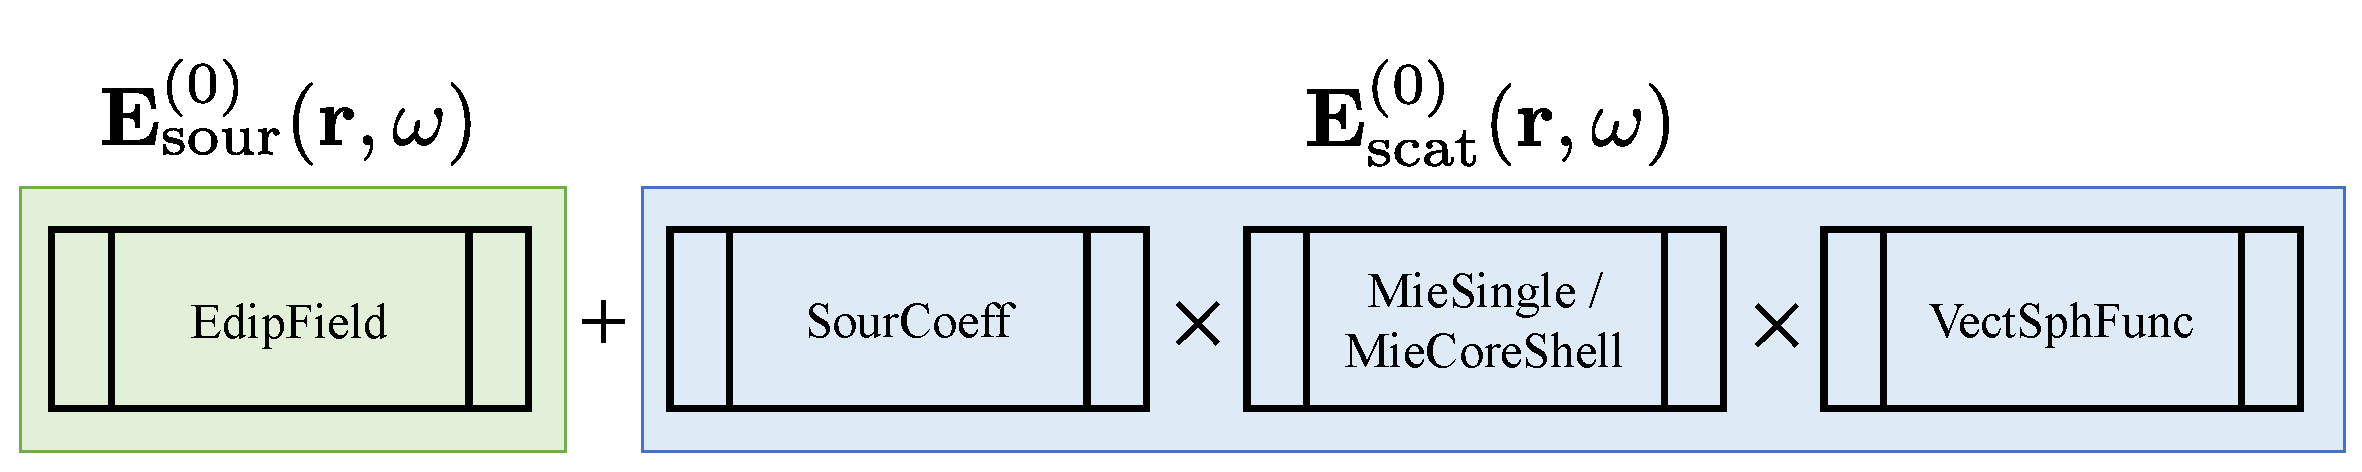
\includegraphics[width=1\textwidth]{Figures/schematic illustration.pdf}
    \caption{Conceptual illustration of calculating the total electric field in the zeroth region. \cfont{EdipField}, \cfont{SourCoeff}, \cfont{MieSingle}/\cfont{MieCoreShell}, and \cfont{VectSphFunc} are the MATLAB functions. These functions will be introduced afterward.}
    \label{illust_of_E_calc}
    \end{center}
\end{figure*}
%
\subsectiontoc{Singularity of Free-Space Dyadic Green's Function}
In Eq.~(\ref{Eq:EdipoleExpand}), we have shown the electric field of an electric point dipole can be expressed by
\begin{align}
    \nonumber
    \mathbf{E}_\mathrm{sour}^{(0)}(\mathbf{r},\omega) &=
    \begin{cases}
        \displaystyle
        \sum_{nm}\left[q_{nm}\norF{M}_{\mathstrut{nm}}^{(\RomanI)}(k_0r,\theta,\phi)+p_{nm}\norF{N}_{\mathstrut{nm}}^{(\RomanI)}(k_0r,\theta,\phi)\right], & r < r_\mathrm{D}\\
        \displaystyle
        \sum_{nm}\left[s_{nm}\norF{M}_{\mathstrut{nm}}^{(\RomanIII)}(k_0r,\theta,\phi)+r_{nm}\norF{N}_{\mathstrut{nm}}^{(\RomanIII)}(k_0r,\theta,\phi)\right], & r > r_\mathrm{D}\\
    \end{cases}
    .
\end{align}
However, from the viewpoint of numerical calculations, the implementation based on  Eq.~(\ref{Eq:EdipoleExpand}) is pathological for the following two reasons.
First, the expression of Eq.~(\ref{Eq:EdipoleExpand}) cannot describe points when $r=r_\mathrm{D}$ because these points are singularity.
Second, despite Eq.~(\ref{Eq:EdipoleExpand}) is analytical, a summation of infinite series is impossible in numerical calculations.
Moreover, a truncation inevitably leads to the Gibbs phenomenon.
Thus, Eq.~(\ref{Eq:EdipoleExpand}) cannot be directly implemented in programs.
The expression of dipole field in Eq.~(\ref{Eq:EdipoleExpand}) originates from expanding the field at an improper origin.
To deal with this issue, we describe the dipole field by choosing a secondary coordinate (the blue frame) which makes $\mathrm{r}_\mathrm{D}'\rightarrow0$, as shown in Fig.~\ref{fig:limcoord}.
\begin{figure}[!b]
    \centering
    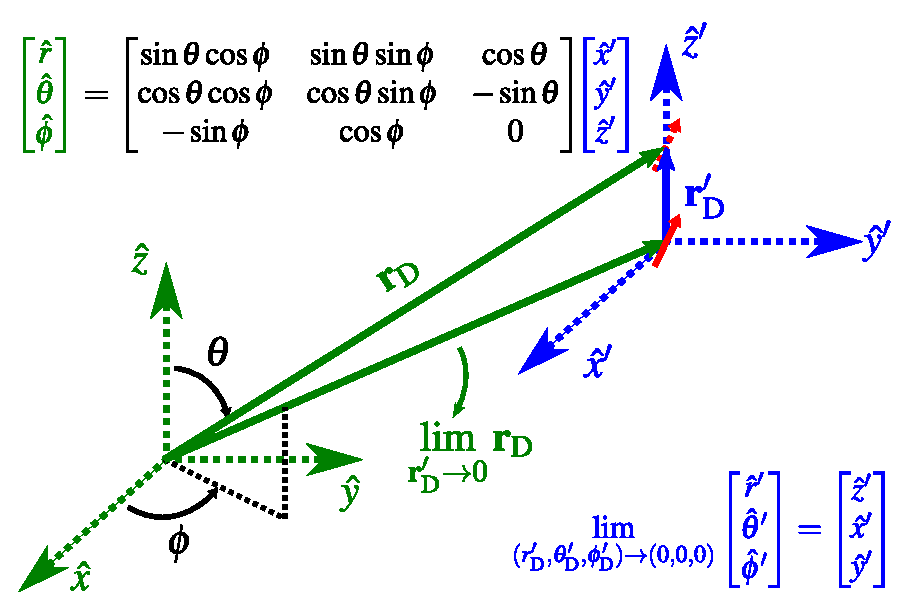
\includegraphics[width=0.85\textwidth]{Figures/limcoordinate.pdf}
    \caption{Primary coordinate (green) and secondary coordinate (blue). Variables with prime is in the representation of the secondary coordinate. The transformation of unit vectors between two coordinates is expressed in the upper left corner. Here, $\hat{r}'$, $\hat{\theta}'$, and $\hat{\phi}'$ correspond to $\hat{z}'$, $\hat{x}'$, and $\hat{y}'$ under the limit.}
    \label{fig:limcoord}
\end{figure}
Here, we add a prime to denote variables under the secondary coordinate, e.g., $\br_\mathrm{D}'$.
Moreover, in the secondary coordinate, we additionally require $\mathrm{r}_\mathrm{D}'$ approaches to zero along the z axis, i.e.,  $(r_\mathrm{D}',\theta_\mathrm{D}',\phi_\mathrm{D}')\rightarrow(0,0,0)$, in order to define and apply the direction of spherical coordinate at the origin.
The advantages of describing the dipole field in the secondary coordinate, the singularity is shrunk to $r_\mathrm{D}'=0$ and the summation of infinite series becomes a summation of finite series under the secondary coordinate.
To acquire the dipole field expressed in the primary coordinate, all we need is to evaluate the coefficients
\begin{align}
    &\lim_{\br_\mathrm{D}'\rightarrow0}r_{nm} = 
    ik_0^3\epsilon_0^{-1}(-1)^m\mathbf{p}_\mathrm{D}^{(0)}(\omega)\cdot\lim_{\br_\mathrm{D}'\rightarrow0}\norF{N}_{n(-m)}^{(\RomanI)}(k_0r_\mathrm{D}',\theta_\mathrm{D}',\phi_\mathrm{D}'),\\
    &\lim_{\br_\mathrm{D}'\rightarrow0}s_{nm} = 
    ik_0^3\epsilon_0^{-1}(-1)^m\mathbf{p}_\textrm{D}^{(0)}(\omega)\cdot\lim_{\br_\mathrm{D}'\rightarrow0}\norF{M}_{n(-m)}^{(\RomanI)}(k_0r_\mathrm{D}',\theta_\mathrm{D}',\phi_\mathrm{D}'),
\end{align}
then do the coordinate transformation $\mathcal{R}(\theta,\phi,\theta',\phi')$,
\begin{align}
    \begin{bmatrix}
    \hat{r}\\ \hat{\theta}\\ \hat{\phi}
    \end{bmatrix}=\mathcal{R}(\theta,\phi,\theta',\phi')
    \begin{bmatrix}
    \hat{r}'\\ \hat{\theta}'\\ \hat{\phi}'
    \end{bmatrix}
    \xrightarrow{\phi=\phi'}
    \begin{bmatrix}
    \cos(\theta'-\theta) & -\sin(\theta'-\theta) & 0 \\
    \sin(\theta'-\theta) & \cos(\theta'-\theta) & 0 \\
    0 & 0 & 1
    \end{bmatrix}
    \begin{bmatrix}
    \hat{r}'\\ \hat{\theta}'\\ \hat{\phi}'
    \end{bmatrix}
\end{align}
First, we evaluate the values of $r_{nm}$ and $s_{nm}$ under the secondary coordinate.
According to Eq.~(\ref{Eq:Mlim}) in \blue{Appendix G}, we obtain that $s_{nm}=0$ ($\mathbf{r}_\mathrm{D}\rightarrow0,~\forall n,m$).
On the other hand, by using Eq.~(\ref{Eq:Nlim}),
the only nonzero term of $r_{nm}$ for a linear-polarized electric point dipole aligned to z axis  [$\mathbf{p}_\mathrm{D}^{(0)}(\omega)=p_\mathrm{D}^{(0)}(\omega)~\hat{z}'=p_\mathrm{D}^{(0)}(\omega)~\hat{r}'$] is
\begin{align}
    \lim_{\mathbf{r}'_\mathrm{D}\rightarrow0}r_{10}&=
    \frac{ik_0^3}{\epsilon_0}\frac{1}{\sqrt{2f_{10}}}\frac{2}{3}P_1^m(1)\cdot p_\mathrm{D}^{(0)}(\omega)=
    \frac{ik_0^3}{\epsilon_0}\left[\frac{1}{6\pi}\right]^{1/2} p_\mathrm{D}^{(0)}(\omega).
\end{align}
Thus, the electric field of a z-polarized point dipole in the new spherical coordinate becomes
\begin{align}
    \mathbf{E}_\mathrm{z-dip}^{'(0)}(\mathbf{r}',\omega)= r_{10}\norF{N}_{\mathstrut{10}}^{(\RomanIII)}(k_0r',\theta',\phi')
    &=\frac{p_\mathrm{D}^{(0)}(\omega)}{4\pi\epsilon_0}ik_0^3\mathbf{N}_{\mathstrut{10}}^{(\RomanIII)}(k_0r',\theta',\phi')
    \label{Eq:zdipoleimp}
\end{align}
For a x-polarized electric point dipole, $\mathbf{p}_\mathrm{D}^{(0)}(\omega)=p_\mathrm{D}^{(0)}(\omega)~\hat{x}'=p_\mathrm{D}^{(0)}(\omega)~\hat{\theta}'$, the nonzero terms of $r_{nm}$ are
\begin{subequations}
    \begin{align}
        \lim_{\mathbf{r}_\mathrm{D}'\rightarrow0}r_{11}=
        \frac{ik_0^3}{\epsilon_0}\frac{-1}{\sqrt{2f_{1(-1)}}}\frac{2}{3}\tau_{1(-1)}(0)\cdot p_\mathrm{D}^{(0)}(\omega)=-
        \frac{ik_0^3}{\epsilon_0}\left[\frac{1}{12\pi}\right]^{1/2} p_\mathrm{D}^{(0)}(\omega)\\
        \lim_{\mathbf{r}_\mathrm{D}'\rightarrow0}r_{1(-1)}=
        \frac{ik_0^3}{\epsilon_0}\frac{-1}{\sqrt{2f_{11}}}\frac{2}{3}\tau_{11}(0)\cdot p_\mathrm{D}^{(0)}(\omega)=
        \frac{ik_0^3}{\epsilon_0}\left[\frac{1}{12\pi}\right]^{1/2} p_\mathrm{D}^{(0)}(\omega)
    \end{align}    
\end{subequations}
The electric field of a x-polarized point dipole in the new spherical coordinate reads
\begin{align}
    \mathbf{E}_\mathrm{x-dip}^{'(0)}(\mathbf{r}',\omega)
    &=\frac{p_\mathrm{D}^{(0)}(\omega)}{4\pi\epsilon_0}ik_0^3
    \cdot\frac{1}{2}\left[
    \mathbf{N}_{\mathstrut{1(-1)}}^{(\RomanIII)}(k_0r',\theta',\phi')-
    \mathbf{N}_{\mathstrut{11}}^{(\RomanIII)}(k_0r',\theta',\phi')
    \right]
    \label{Eq:xdipoleimp}
\end{align}
In the same way, for a y-polarized electric point dipole [$\mathbf{p}_\mathrm{D}^{(0)}(\omega)=p_\mathrm{D}^{(0)}(\omega)~\hat{y}'=p_\mathrm{D}^{(0)}(\omega)~\hat{\phi}'$], the nonzero terms of $r_{nm}$ are
\begin{subequations}
    \begin{align}
        \lim_{\mathbf{r}_\mathrm{D}'\rightarrow0}r_{11}=
        \frac{ik_0^3}{\epsilon_0}\frac{-1}{\sqrt{2f_{1(-1)}}}\frac{2}{3}i\pi_{1(-1)}(0)\cdot p_\mathrm{D}^{(0)}(\omega)=
        \frac{ik_0^3}{\epsilon_0}\cdot i\left[\frac{1}{12\pi}\right]^{1/2} p_\mathrm{D}^{(0)}(\omega),\\
        \lim_{\mathbf{r}_\mathrm{D}'\rightarrow0}r_{1(-1)}=
        \frac{ik_0^3}{\epsilon_0}\frac{-1}{\sqrt{2f_{11}}}\frac{2}{3}i\pi_{11}(0)\cdot p_\mathrm{D}^{(0)}(\omega)=
        \frac{ik_0^3}{\epsilon_0}\cdot i\left[\frac{1}{12\pi}\right]^{1/2} p_\mathrm{D}^{(0)}(\omega),
    \end{align}    
\end{subequations}
and the electric field is
\begin{align}
    \mathbf{E}_\mathrm{y-dip}^{'(0)}(\mathbf{r}',\omega)
    &=\frac{p_\mathrm{D}^{(0)}(\omega)}{4\pi\epsilon_0}ik_0^3
    \cdot\frac{i}{2}\left[
    \mathbf{N}_{\mathstrut{1(-1)}}^{(\RomanIII)}(k_0r',\theta',\phi')+
    \mathbf{N}_{\mathstrut{11}}^{(\RomanIII)}(k_0r',\theta',\phi')
    \right]
    \label{Eq:ydipoleimp}
\end{align}
Equations~(\ref{Eq:zdipoleimp}),~(\ref{Eq:xdipoleimp}),~and~(\ref{Eq:ydipoleimp}) are the final forms used in the numerical calculations. 
Generally, for an arbitrary linear-polarized electric dipole,
\begin{align}
    \mathbf{p}_\mathrm{D}^{(0)}(\omega)=p_\mathrm{D}^{(0)}(\omega)~\hat{p}
    &=p_\mathrm{D,x'}^{(0)}(\omega)~\hat{x}'+p_\mathrm{D,y'}^{(0)}(\omega)~\hat{y}'+p_\mathrm{D,z'}^{(0)}(\omega)~\hat{z}'\\
    \label{Eq:pspherical}
    &=p_\mathrm{D,x'}^{(0)}(\omega)~\hat{\theta}'+p_\mathrm{D,y'}^{(0)}(\omega)~\hat{\phi}'+p_\mathrm{D,z'}^{(0)}(\omega)~\hat{r}',
\end{align}
the electric field is expressed as
\begin{align}
    \nonumber
    \mathbf{E}^{'(0)}(\mathbf{r}',\omega)=&
    \frac{p_\mathrm{D,z'}^{(0)}(\omega)}{4\pi\epsilon_0}ik_0^3\cdot\mathbf{N}_{\mathstrut{10}}^{(\RomanIII)}(k_0r',\theta',\phi')\vphantom{\frac{1}{2}}\\
    \nonumber
    +&\frac{p_\mathrm{D,x'}^{(0)}(\omega)}{4\pi\epsilon_0}ik_0^3\cdot
    \frac{1}{2}\left[
    \mathbf{N}_{\mathstrut{1(-1)}}^{(\RomanIII)}(k_0r',\theta',\phi')-
    \mathbf{N}_{\mathstrut{11}}^{(\RomanIII)}(k_0r',\theta',\phi')
    \right]\\
    +&\frac{p_\mathrm{D,y'}^{(0)}(\omega)}{4\pi\epsilon_0}ik_0^3\cdot
    \frac{i}{2}\left[
    \mathbf{N}_{\mathstrut{1(-1)}}^{(\RomanIII)}(k_0r',\theta',\phi')+
    \mathbf{N}_{\mathstrut{11}}^{(\RomanIII)}(k_0r',\theta',\phi')
    \right].
    \label{Eq:arbitrarydip}
\end{align}
Finally, to express the original electric field, a coordinate transformation back to the primary coordinate is needed
\begin{align}
    \mathbf{E}^{'(0)}(\mathbf{r}',\omega)\longmapsto\mathbf{E}^{(0)}(\mathbf{r},\omega)=\mathcal{R}(\theta,\phi,\theta',\phi')\cdot\mathbf{E}^{'(0)}(\mathbf{r}-\mathbf{r}_\mathrm{D},\omega).
\end{align}
%\begin{figure}[!t]
%    \centering
%    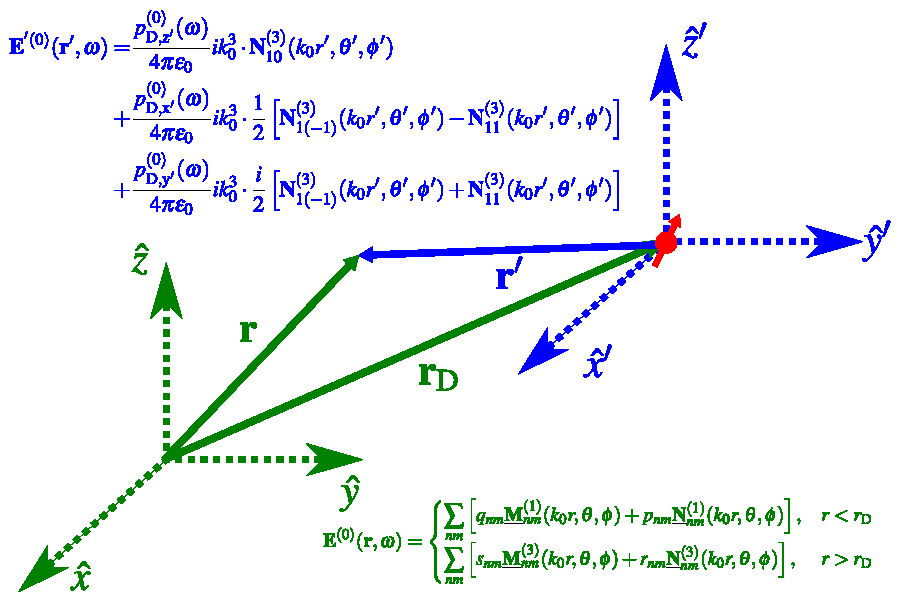
\includegraphics[width=0.6\textwidth]{Figures/2coordinate.pdf}
%    \caption{Schematic illustration of the electric field expressed by two different %reference frame (green and blue). }
%    \label{fig:2coordinate}
%\end{figure}%
To check whether Eq.~(\ref{Eq:arbitrarydip}) is correct, we continue the simplification.
The first vector spherical function in Eq.~(\ref{Eq:arbitrarydip}) can be explicitly expressed as
\begin{align}
    \nonumber
    \vb{N}_{10}^{(\RomanIII)}(k_0r',\theta',\phi')&=
    \frac{h_1^{(1)}(k_0r')}{k_0r'} \cdot 2P_1^0(\cos{\theta}')~\hat{r}'+
    \frac{1}{k_0r'}\frac{\diff \xi_1(k_0r')}{\diff(k_0r')}\cdot \tau_{10}(\theta')~\hat{\theta}'\\
    \nonumber
    &=
    \frac{h_1^{(1)}(k_0r')}{k_0r'} \cdot 2\cos\theta'~\hat{r}'-
    \frac{1}{k_0r'}\frac{\diff \xi_1(k_0r')}{\diff(k_0r')}\cdot \sin\theta'~\hat{\theta}'\\
    &=
    \frac{h_1^{(1)}(k_0r')}{k_0r'} \cdot \left(3\cos\theta'~\hat{r}'-\cos\theta'~\hat{r}'\right)-
    \frac{1}{k_0r'}\frac{\diff \xi_1(k_0r')}{\diff(k_0r')}\cdot \sin\theta'~\hat{\theta}',
    \label{Eq:E'first}
\end{align}
where $P_1^0(\cos\theta')=\cos\theta'$ and $\tau_{10}(\theta')=-\sin\theta'$.
Here, we use the following identities to express the radial functions,
\begin{subequations}
    \begin{align}
        \frac{h_n^{(1)}(k_0r')}{k_0r'} &= -\frac{e^{ik_0r'}}{(k_0r')^2}\left(1+\frac{i}{k_0r'}\right)= \frac{e^{ik_0r'}}{ik_0^3r'}\left(\frac{1}{r'^2}-\frac{ik_0}{r'}\right),\\
        \frac{1}{k_0r'}\frac{\diff\xi_1(k_0r')}{\diff(k_0r')} &=-\frac{ie^{ik_0r'}}{k_0r'}\left(1+\frac{i}{k_0r'}-\frac{1}{(k_0r')^2}\right)
        =\frac{e^{ik_0r'}}{ik_0^3r'}\left(k_0^2+\frac{ik_0}{r'}-\frac{1}{r'^2}\right),
    \end{align}
\end{subequations}
and apply to Eq.~(\ref{Eq:E'first}), the vector spherical function becomes
\begin{align}
    \nonumber
    \vb{N}_{10}^{(\RomanIII)}(k_0r',\theta',\phi')
    &=
    \frac{h_1^{(1)}(k_0r')}{k_0r'} \cdot \left(3\cos\theta'~\hat{r}'-\cos\theta'~\hat{r}'\right)-
    \frac{1}{k_0r'}\frac{\diff \xi_1(k_0r')}{\diff(k_0r')}\cdot \sin\theta'~\hat{\theta}'\\
    \nonumber
    &=
    \frac{e^{ik_0r'}}{ik_0^3r'}\left\{\left(\frac{1}{r'^2}-\frac{ik_0}{r'}\right)\left[3\cos\theta'~\hat{r}'-\left(\cos\theta'~\hat{r}'-\sin\theta'~\hat{\theta}'\right)\right]-
    k_0^2\cdot \sin\theta'~\hat{\theta}'\right\}\\
    \nonumber
    &=
    \frac{e^{ik_0r'}}{ik_0^3r'}\left\{
    \left(\frac{1}{r'^2}-\frac{ik_0}{r'}\right)\left[3\hat{r}'(\hat{r}'\cdot\hat{z}')-\hat{z}'\right]+k_0^2~\hat{\theta}'(\hat{\theta}'\cdot\hat{z}')
    \right\}\\
    &=
    \frac{e^{ik_0r'}}{ik_0^3r'}\left\{
    \left(\frac{1}{r'^2}-\frac{ik_0}{r'}\right)\left[3\hat{r}'(\hat{r}'\cdot\hat{z}')-\hat{z}'\right]+k_0^2\left[\hat{z}'-\hat{r}'(\hat{r}'\cdot\hat{z}')\right]
    \right\}
    \label{Eq:N10}
\end{align}
In the derivation of Eq.~(\ref{Eq:N10}), we use the relation,
$\hat{z}'=\hat{r}'(\hat{r}'\cdot\hat{z}')+\hat{\theta}'(\hat{\theta}'\cdot\hat{z}')+\hat{\phi}'(\hat{\phi}'\cdot\hat{z}')=\cos\theta'~\hat{r}'-\sin\theta'~\hat{\theta}'$.
Combining with Eq.~(\ref{Eq:zdipoleimp}), we get
\begin{align}
    \nonumber
    \mathbf{E}_\mathrm{z-dip}^{'(0)}(\mathbf{r}',\omega)&=
    \frac{p_\mathrm{D}^{(0)}(\omega)}{4\pi\epsilon_0}ik_0^3\mathbf{N}_{\mathstrut{10}}^{(\RomanIII)}(k_0r',\theta',\phi')\\
    &=
    \frac{p_\mathrm{D}^{(0)}(\omega)}{4\pi\epsilon_0}
    \frac{e^{ik_0r'}}{r'}\left\{
    \left(\frac{1}{r'^2}-\frac{ik_0}{r'}\right)\left[3\hat{r}'(\hat{r}'\cdot\hat{z}')-\hat{z}'\right]+k_0^2\left[\hat{z}'-\hat{r}'(\hat{r}'\cdot\hat{z}')\right]
    \right\},
    \label{Eq:Edipolevac}
\end{align}
which is the electric field of a z-polarized dipole.
In the same way, the vector spherical functions of the x-polarized dipole and the z-polarized dipole can be expressed as
\begin{align}
    \nonumber
    &\frac{1}{2}\left[\mathbf{N}_{\mathstrut{1(-1)}}^{(\RomanIII)}(k_0r',\theta',\phi')-\mathbf{N}_{\mathstrut{11}}^{(\RomanIII)}(k_0r',\theta',\phi')\right]\\
    =&\left[
    \frac{h_1^{(1)}(k_0r')}{k_0r'}\cdot2\sin\theta'\cos\phi'~\hat{r}'+
    \frac{1}{k_0r'}\frac{\diff\xi_1(k_0r')}{\diff(k_0r')}\cdot\left(\cos\theta'\cos\phi'~\hat{\theta}'-\sin\phi'~\hat{\phi}'\right)\right]\\
    \nonumber
    =&\left\{
    \frac{h_1^{(1)}(k_0r')}{k_0r'}\cdot2\hat{r}'(\hat{r}'\cdot\hat{x}')+
    \frac{1}{k_0r'}\frac{\diff\xi_1(k_0r')}{\diff(k_0r')}\cdot
    \left[\hat{\theta}'(\hat{\theta}'\cdot\hat{x}')+\hat{\phi}'(\hat{\phi}'\cdot\hat{x}')\right]\right\}\\
    \label{Eq:N11-}
    =&
    \frac{e^{ik_0r'}}{ik_0^3r'}\left\{\left(\frac{1}{r'^2}-\frac{ik_0}{r'}\right)
    \left[3\hat{r'}(\hat{r}'\cdot\hat{x}')-\hat{x}'\right]+k_0^2
    \left[\hat{x}'-\hat{r}'(\hat{r}'\cdot\hat{x}')\right]\right\},
\end{align}
and 
\begin{align}
    \nonumber
    &\frac{i}{2}\left[\mathbf{N}_{\mathstrut{1(-1)}}^{(\RomanIII)}(k_0r',\theta',\phi')+\mathbf{N}_{\mathstrut{11}}^{(\RomanIII)}(k_0r',\theta',\phi')\right]\\
    =&\left[
    \frac{h_1^{(1)}(k_0r')}{k_0r'}\cdot2\sin\theta'\sin\phi'~\hat{r}+
    \frac{1}{k_0r'}\frac{\diff\xi_1(k_0r')}{\diff(k_0r')}\cdot\left(\cos\theta'\sin\phi'~\hat{\theta}'+\cos\phi'~\hat{\phi}'\right)\right]\\
    \nonumber
    =&\left\{
    \frac{h_1^{(1)}(k_0r')}{k_0r'}\cdot2\hat{r}'(\hat{r}'\cdot\hat{y}')+
    \frac{1}{k_0r'}\frac{\diff\xi_1(k_0r')}{\diff(k_0r')}\cdot
    \left[\hat{\theta}'(\hat{\theta}'\cdot\hat{y}')+\hat{\phi}'(\hat{\phi}'\cdot\hat{y}')\right]\right\}\\
    \label{Eq:N11+}
    =&
    \frac{e^{ik_0r'}}{ik_0^3r'}\left\{\left(\frac{1}{r'^2}-\frac{ik_0}{r'}\right)
    \left[3\hat{r}'(\hat{r}'\cdot\hat{y}')-\hat{y}'\right]+k_0^2
    \left[\hat{y}'-\hat{r}'(\hat{r}'\cdot\hat{y}')\right]\right\},
\end{align}
respectively.
In Eq.~(\ref{Eq:N11-}) and (\ref{Eq:N11+}), the angular functions are $P_1^{-1}(\cos\theta)=-P_1^{1}(\cos\theta)=\sin\theta$, $\tau_{1(-1)}(\theta)=-\tau_{11}(\theta)=\cos\theta$, and $\pi_{1(-1)}(\theta)=\pi_{11}(\theta)=-1$. In addition, the Cartesian unit vectors in the representation of spherical coordinate are $\hat{x}'=\sin\theta'\cos\phi'~\hat{r}'+\cos\theta'\cos\phi'~\hat{\theta}'-\sin\phi'~\hat{\phi}'$ and
$\hat{y}'=\sin\theta'\sin\phi'~\hat{r}'+\cos\theta'\sin\phi'~\hat{\theta}'+\cos\phi'~\hat{\phi}'$. The electric field of the x-polarized (y-polarized) dipole is
similar to Eq.~(\ref{Eq:Edipolevac}), the only difference is the dipole direction.
Finally, applying Eqs.~(\ref{Eq:N10}),~(\ref{Eq:N11-}), and~(\ref{Eq:N11+}) to Eq.~(\ref{Eq:arbitrarydip}), the electric field generated by a dipole under the secondary coordinate reads
\begin{align}
    \mathbf{E}_\mathrm{dip}^{'(0)}(\mathbf{r}',\omega)
    =&
    \frac{p_\mathrm{D}^{(0)}(\omega)}{4\pi\epsilon_0}
    \frac{e^{ik_0r'}}{r'}\left\{
    \left(\frac{1}{r'^2}-\frac{ik_0}{r'}\right)\left[3\hat{r}'(\hat{r}'\cdot\hat{p}')-\hat{p}'\right]+k_0^2\left[\hat{p}'-\hat{r}'(\hat{r}'\cdot\hat{p}')\right]
    \right\},
\end{align}
which is indeed the textbook form of the electric field generated by an electric point dipole.
On the basis of the above description, the implementation is presented as follows,
\lstinputlisting[caption={Computation of electric dipole field},captionpos=b]{code/EdipField.m}
Note that we build the function \cfont{EdipField} in Gaussian unit, which makes difference from the above derivation (SI unit). 
In addition, the coordinate transform $\mathcal{R}(\theta,\phi,\theta',\phi')$ is accomplished by \cfont{S2S}, as shown in Func.~\ref{F:S2S}.
For the sake of convenience, we request that $\phi=\phi'$, implying the dipole locates on the $z$ axis.
\lstinputlisting[caption={Coordinate transformation between two spherical coordinates},captionpos=b,label={F:S2S}]{code/S2S.m}
\newpage
\subsectiontoc{Numerical Precision of Vector Spherical Functions}
The precision of vector spherical functions determines whether computations are converged, where
the vector spherical functions are the product of spherical Bessel functions and vector spherical harmonics,
\begin{align}
    \label{Eq:norM}
    \norF{M}_{nm}^{(j)} (k_ir,\theta,\phi) 
    &= z_n(k_ir)\left[ i\norF{\pi}_{nm}(\theta)\hat{\theta}-\norF{\tau}_{nm}(\theta)\hat{\phi} \right]\frac{1}{\sqrt{2\pi}}e^{im\phi},\\
    \nonumber
    \norF{N}_{nm}^{(j)} (k_ir,\theta,\phi)
    &= \frac{z_n(k_ir)}{k_ir} \cdot n(n+1)\underline{P}_n^m(\cos{\theta})\frac{1}{\sqrt{2\pi}}e^{im\phi}\hat{r}\\
    \label{Eq:norN}
    &~+ \frac{1}{k_ir}\frac{\diff Z_n(k_ir)}{\diff(k_ir)}\cdot\left[ \norF{\tau}_{nm}(\theta)\hat{\theta}+i\norF{\pi}_{nm}(\theta)\hat{\phi} \right]\frac{1}{\sqrt{2\pi}}e^{im\phi}.
\end{align}
Note that $j=\NRomanI$ for $z_n(k_ir)=j_n(k_ir)$ and $Z_n(k_ir)=\psi_n(k_ir)$, and $j=\NRomanIII$ for $z_n(k_ir)=h_n^{(1)}(k_ir)$ and $Z_n(k_ir)=\xi_n(k_ir)$.
Here, we construct two MATLAB functions to compute the radial and angular functions.
In the radial part, we need to cope with spherical Bessel (Hankel) functions $j_n(k_ir)$ [$h_n^{(1)}(k_ir)$] and the derivatives of Raccati-Bessel (-Hankel) functions $\psi_{n}'(k_ir)$ [$\xi_{n}'(k_ir)$].
The angular part includes exponential functions and the following functions, 
\begin{subequations}
    \begin{align}
        \underline{P}_n^m(\cos\theta)&=
        \left[\frac{(2n+1)(n-\abs{m}!)}{2n(n+1)(n+\abs{m}!)}\right]^{1/2}
        P_n^m(\cos\theta)\\
        \norF{\pi}_{nm}(\theta)&=
        \left[\frac{(2n+1)(n-\abs{m}!)}{2n(n+1)(n+\abs{m}!)}\right]^{1/2}
        \pi_{nm}(\theta)\\
        \norF{\tau}_{nm}(\theta)&=
        \left[\frac{(2n+1)(n-\abs{m}!)}{2n(n+1)(n+\abs{m}!)}\right]^{1/2}
        \tau_{nm}(\theta).
    \end{align}
    \label{Eq:normPolar}
\end{subequations}

\subsubsectiontoc{Radial Functions}
We need to compute the following three radial functions: (1) spherical Bessel (Hankel) functions, (2) Riccati-Bessel (Hankel) functions, and (3) derivatives of Riccati-Bessel (Hankel) functions.
Apart from the built-in functions in MATLAB, we use the algorithm\cite{crandall1997computation} to calculate these functions, where a MATLAB version source code is presented in Func.~\ref{F:SphBessel}.
In \cfont{SphBessel}, the two additional sub-functions, \cfont{sbesselc} and \cfont{rcbesselc}, are called on line 14, 44, and 54.
\cfont{sbesselc} and \cfont{rcbesselc} are form the reference\cite{crandall1997computation} that are originally coding in Fortran language.
Here, we translate them to the MATLAB version and present in Funcs.~\ref{F:sbesselc} and \ref{F:rcbesselc}.
Note that the three auxiliary functions, \cfont{MSTA1}, \cfont{MSTA2}, and \cfont{envj}, are called in \cfont{sbesselc} (Func.~\ref{F:sbesselc}) and  \cfont{rcbesselc} (Func.~\ref{F:rcbesselc}).
These auxiliary functions are presented in Funcs.~\ref{F:MSTA1} to \ref{F:envj}.
\lstinputlisting[caption={Computation of spherical Bessel functions and their associated functions},captionpos=b,label={F:SphBessel}]{code/RadialPart/SphBessel.m}
\newpage
\lstinputlisting[caption={Computation of spherical Bessel (Hankel) functions},captionpos=b,label={F:sbesselc}]{code/RadialPart/sbesselc.m}
\newpage
\lstinputlisting[caption={Computation of Riccati-Bessel (-Hankel) functions},captionpos=b,label={F:rcbesselc}]{code/RadialPart/rcbesselc.m}
\newpage
\lstinputlisting[caption={Auxiliary function \cfont{MSTA1}},captionpos=b,label={F:MSTA1}]{code/RadialPart/MSTA1.m}
%\newpage
\lstinputlisting[caption={Auxiliary function \cfont{MSTA2}},captionpos=b,label={F:MSTA2}]{code/RadialPart/MSTA2.m}
\lstinputlisting[caption={Auxiliary function \cfont{envj}},captionpos=b,label={F:envj}]{code/RadialPart/envj.m}

\newpage
\subsubsectiontoc{Angular Functions}
As shown in Eq.~(\ref{Eq:normPolar}), the angular functions are related to associated Legendre polynomials,
\begin{subequations}
    \begin{align}
        \underline{P}_n^m(\cos\theta)&=
        \left[\frac{(2n+1)(n-\abs{m})!}{2n(n+1)(n+\abs{m})!}\right]^{1/2}
        P_n^m(\cos\theta),\\
        \norF{\pi}_{nm}(\theta)&=
        \left[\frac{(2n+1)(n-\abs{m})!}{2n(n+1)(n+\abs{m})!}\right]^{1/2}
        \frac{m}{\sin\theta}P_n^m\left(\cos{\theta}\right),\\
        \norF{\tau}_{nm}(\theta)&=
        \left[\frac{(2n+1)(n-\abs{m})!}{2n(n+1)(n+\abs{m})!}\right]^{1/2}
        \frac{\diff}{\diff\theta}\left[P_n^m\left(\cos{\theta}\right)\right].
    \end{align}
\end{subequations}
Naively, we can use the recurrence relations of associated Legendre polynomials to compute these functions, but the function error would cumulatively grow if $n$ is large.
To keep the numerical precision, we utilize the relations based on Wigner D functions [$D_{m'm}^n(\theta)$],
\begin{subequations}
\begin{align}
    \label{norP}
    \underline{P}_n^m(\cos\theta) &=
    \left[\frac{2n+1}{2n(n+1)}\right]^{1/2}D_{m0}^n(0,\theta,0)\\
    \label{norPi}
    \norF{\pi}_{nm}(\theta) &= -\left[\frac{2n+1}{8}\right]^{1/2}\left[\vphantom{\frac{1}{1}} D_{m,1}^n(0,\theta,0)+D_{m,-1}^n(0,\theta,0) \right],\\
    \label{norTau}
    \norF{\tau}_{nm}(\theta) &= -\left[\frac{2n+1}{8}\right]^{1/2}\left[\vphantom{\frac{1}{1}} D_{m,1}^n(0,\theta,0)-D_{m,-1}^n(0,\theta,0) \right].
\end{align}
\end{subequations}
Based on Eq.~(\ref{norP}), we will prove that  Eqs.~(\ref{norPi}) and (\ref{norTau}) are correct after the introduction of Wigner D functions, which is rarely discussed in present literature.
Function~(\ref{F:NormTauPiP}) demonstrates the computation of Eqs.~(\ref{norP}) to (\ref{norTau}). \cfont{NormTauPiP} requests three inputs, \cfont{nmax}, \cfont{theta}, and \cfont{order}.
Literally, \cfont{nmax} indicates the highest expansion order and \cfont{theta} is the variable of Wigner D functions.
\cfont{order} is a string which makes the output order become `normal' order or `reversed' order.
Also, it can be found that \cfont{NormTauPiP} outputs a structure array, \cfont{NAng}, including \cfont{NTau}, \cfont{NPi}, and \cfont{NP}.
The three arrays save the output of $\norF{\tau}_{nm}(\theta)$, $\norF{\pi}_{nm}(\theta)$, and $\underline{P}_{nm}(\theta)$, respectively.
On line 9 in \cfont{NormTauPiP}, the computation of Wigner d functions is done by \cfont{Wigner\_d}, as shwon in Func.~\ref{F:Wigner_d}.
To get the numerically high-precision Wigner D functions, a algorithm based on numerical diagonalization is adopted\cite{feng2015high}.
\lstinputlisting[caption={Computation of $\norF{\tau}_{nm}(\theta)$, $\norF{\pi}_{nm}(\theta)$, and $\underline{P}_{n}^m(\cos\theta)$},label={F:NormTauPiP}]{code/NormTauPiP.m}
\newpage
\noindent
Wigner D functions are well-known in angular momentum theory.
These functions describe an Euler rotation, and the order of fixed axes is z-y-z.
Wigner D functions are defined as\footnote{We use the same symbol $m$ when defining $\norF{\pi}_{nm}(\theta)$, $\norF{\tau}_{nm}(\theta)$, and Wigner D (d) functions since all of them are associated with the degree of freedom of the azimuthal angle. Please do not be confused when we introduce the properties of Wigner D (d) functions with the convention symbols.}
\begin{align}
    D_{m',m}^j(\alpha,\beta,\gamma) \equiv \bra{j,m'}\hat{R}(\alpha,\beta,\gamma)\ket{j,m}
    =\bra{j,m'}e^{-i\alpha \hat{J}_z}e^{-i\beta \hat{J}_y}e^{-i\gamma \hat{J}_z}\ket{j,m},
\end{align}
where $\hat{R}(\alpha,\beta,\gamma)$ refers to a rotation operator. $\hat{J}_z$ and $\hat{J}_y$ (also, $\hat{J}_x$) are the generators of the Lie group of SO(3), and the three generators form a Lie algebra $\mathfrak{so}(3)$, 
\begin{align}
    \left[ \hat{J}_i,\hat{J}_j \right] = i\epsilon_{ijk}\hat{J}_k,
    \hspace{1 cm}
    i,j,k = \{\mathrm{x,y,z}\}.
\end{align}
$\epsilon_{ijk}$ is a skew-symmetric tensor (or in other words, Levi-Civita symbol).
This algebra is isomorphic to the orbital angular momentum operators in quantum mechanics.
When we do the following operations on the eigenstate $\ket{j,m}$, it yields:
\begin{align}
    \hat{J}_\mathrm{z}\ket{j,m} = m\ket{j,m}, \hspace{1 cm}
    \hat{J}^2\ket{j,m} = j(j+1)\ket{j,m}, \hspace{1 cm} \hat{J}^2 = \hat{J}_\mathrm{x}^2+\hat{J}_\mathrm{y}^2+\hat{J}_\mathrm{z}^2.
\end{align}
It is obvious that
\begin{align}
    \nonumber
    \bra{j,m'}e^{-i\alpha \hat{J}_z}e^{-i\beta \hat{J}_y}e^{-i\gamma \hat{J}_z}\ket{j,m}
    &=e^{-im'\alpha}\bra{j,m'}e^{-i\beta \hat{J}_y}\ket{j,m}e^{-im\gamma}\\
    &\equiv e^{-im'\alpha}d_{m',m}^j(\beta)e^{-im\gamma},
\end{align}
where we define that $d_{m',m}^j(\beta)\equiv\bra{j,m'}e^{-i\beta \hat{J}_y}\ket{j,m}$.
Thus, the equation $D_{m',m}^j(0,\beta,0)=d_{m',m}^j(\beta)$ holds.
Here, we would like to emphasize that $m$ is the eigenvalues of $\hat{J}_\mathrm{z}$ by convention.
In addition, we can also define another complete eigenbasis about $\hat{J}_\mathrm{y}$,
\begin{align}
    \mathbf{I}=\sum_{\mu-j}^j\ket{j,\mu}\bra{j,\mu},
\end{align}
and $\mu$ denotes the eigenvalue along y axis. 
Inserting this complete relation, the equation becomes:
\begin{align}
    d_{m',m}^{j}(\theta) &= \sum_\mu{\bra{j,m'}\ket{j,\mu}e^{-i\theta \hat{J}_\mathrm{y}}\bra{j,\mu}\ket{j,m}}
    = \sum_\mu{e^{-i\theta \mu}\bra{j,m'}\ket{j,\mu}\bra{j,\mu}\ket{j,m}}.
\end{align}
In the matrix representation, we have
\begin{align}
    \label{dmatrix}
    \mathbf{d}(\theta) =
    \begin{bmatrix}
    d_{-m,-m}^j & d_{-m,-m+1}^j & \cdots & d_{-m,m}^j\\
    d_{-m+1,-m}^j & d_{-m+1,-m+1}^j & \cdots & d_{-m,m}^j\\
    \vdots & \vdots & \ddots & \vdots\\
    d_{m,-m}^j & d_{m,-m+1}^j & \cdots & d_{m,m}^j
    \end{bmatrix}_\mathrm{z}
    = \mathbf{P}\begin{bmatrix}
    e^{i\mu\theta} & 0 & \cdots & 0\\
    0 & e^{i(\mu-1)\theta} & \cdots & 0\\
    \vdots & \vdots &\ddots & 0\\
    0 & 0 & \cdots & e^{-i\mu\theta}
    \end{bmatrix}_\mathrm{y}
    \mathbf{P}^{-1}
\end{align}
According to Eq.~(\ref{dmatrix}), if we get the modal matrix $\mathbf{P}$, we are able to calculate Wigner d functions.
To solve the modal matrix $\mathbf{P}$, we define a pair of ladder operators, $\hat{J}_+\equiv \hat{J}_\mathrm{x}+i\hat{J}_\mathrm{y}$ and $\hat{J}_-\equiv \hat{J}_\mathrm{x}-i\hat{J}_\mathrm{y}$.
When these operators act on the eigenstate $\ket{j,m}$, they return
\begin{align}
    \label{Eq:OpLadd}
    \hat{J}_\pm\ket{j,m} = C_\pm(j,m) \ket{j,m\pm1}, 
\end{align}
where $C_\pm(j,m) = \sqrt{(j\mp m)(j\pm m+1)}$.
The only step we need to do is solve the eigenvalue problem for $\hat{J}_\mathrm{y}$ in the z-basis representation.
The form can obtain from the following formula:
\begin{align}
    \nonumber
    [\hat{J}_\mathrm{y}]_\mathrm{z} &= \frac{1}{2i}(\hat{J}_+-\hat{J}_-)_\mathrm{z}\\ 
    &= \frac{1}{2i}\begin{bmatrix}
    0 & -C_-(j,-j+1) & 0 & \cdots & 0\\
    C_+(j,-j) & 0 & -C_-(j,-j+2) & \cdots & 0\\
    0 & C_+(j,-j+1) & 0 &\cdots & 0\\
    \vdots & \vdots & \vdots & \ddots & -C_-(j,j)\\
    0 & 0 & 0 & \cdots & 0
    \end{bmatrix}_\mathrm{z}
\end{align}
After the diagonalization, we get
\begin{align}
    [\hat{J}_\mathrm{y}]_\mathrm{y} = \mathbf{P}^{-1}[\hat{J}_\mathrm{y}]_\mathrm{z}\mathbf{P} = \begin{bmatrix}
    -\mu & 0 & 0 & \cdots & 0\\
    0 & -\mu+1 & 0 & \cdots & 0\\
    0 & 0 & -\mu+2 &\cdots & 0\\
    \vdots & \vdots & \vdots & \ddots & 0\\
    0 & 0 & 0 & \cdots & \mu
    \end{bmatrix}_y.
\end{align}
Applying $\mathbf{P}$ to Eq.~(\ref{dmatrix}), we can acquire the Wigner d function.
In Func.~\ref{F:Wigner_d}, we show the source code of the algorithm.

\lstinputlisting[caption={Computation of Wigner d functions},captionpos=b,label={F:Wigner_d}]{code/Wigner_d.m}
\newpage

\newpage
\subsubsectiontoc{Vector Spherical Functions}
By calling the functions, \cfont{SphBessel} and \cfont{NormTauPiP}, we are able to construct the basis functions now, which is accomplished by Func.~\ref{F:VectSphField}. 
In \cfont{VectSphField}, components in $\vb{F} = \{\norF{M}_{nm}^{(j)},\norF{N}_{nm}^{(j)}\}$ follow the two-dimensional arrangement if we set the output of \cfont{NormTauPiP} to be `normal' order, 
\begin{align}
    \label{Eq:Fmatrix}
    \small{[\vb{F}]_{nm}^i =}
    \begin{bmatrix}
        F_{1,-1}^i & F_{1,0}^i & F_{1,1}^i & 0 & 0 & \dots &  0\\
        F_{2,-2}^i & F_{2,-1}^i & F_{2,0}^i & F_{2,1}^i & F_{1,2}^i &\dots &  0\\
        \vdots & \vdots & \vdots & \vdots & \vdots & \ddots &  \vdots\\
        F_{n-1,-n+1}^i & F_{n-1,-n+2}^i & F_{n-1,-n+3}^i & F_{n-1,-n+4}^i & F_{n-1,-n+5}^i & \dots & 0\\
        F_{n,-n}^i & F_{n,-n+1}^i & F_{n,-n+2}^i & F_{n,-n+3}^i & F_{n,-n+4}^i & \dots & F_{n,n}^i
    \end{bmatrix}.
\end{align}
Index $i$ indicates the $i$-th component of spherical coordinates.
The elements of $\vb{F}$ in each row store the same order of $n$; for each $n$, a total of $2n+1$ choices for $m$.
Thus, if $n_\mathrm{max}$ is the highest expansion order to $n$, a total of $2(n_\mathrm{max}-n)$ zeros in the rest of each row. 
Note that although the arrangement in Eq.~(\ref{Eq:Fmatrix}) is not conducive to computation efficiency, it is a friendly arrangement for humans to debug.
On the other hand, if we set the output of \cfont{NormTauPiP} to be `reversed' order, the reversed array $\tilde{\vb{F}}$ becomes
\begin{align}
    \label{Eq:Fmatrix_rev}
    \small{[\tilde{\vb{F}}]_{nm}^i =}
    \begin{bmatrix}
        F_{1,1}^i & F_{1,0}^i & F_{1,-1}^i & 0 & 0 & \dots &  0\\
        F_{2,2}^i & F_{2,1}^i & F_{2,0}^i & F_{2,-1}^i & F_{1,-2}^i &\dots &  0\\
        \vdots & \vdots & \vdots & \vdots & \vdots & \ddots &  \vdots\\
        F_{n-1,n-1}^i & F_{n-1,n-2}^i & F_{n-1,n-3}^i & F_{n-1,n-4}^i & F_{n-1,n-5}^i & \dots & 0\\
        F_{n,n}^i & F_{n,n-1}^i & F_{n,n-2}^i & F_{n,n-3}^i & F_{n,n-4}^i & \dots & F_{n,-n}^i
    \end{bmatrix}.
\end{align}
The reversed vector spherical fields are called when calculating the dyadic Green's functions [in practice, expansion coefficients of the electric point dipole, Eq.~(\ref{Eq:EdipoleExpandcoeff})].
\newpage
\lstinputlisting[caption={Generation of Vector Spherical Functions},captionpos=b,label={F:VectSphField}]{code/VectSphField.m}
\newpage
\begin{comment}
\newpage
\subsection{Graveyard}
In the graveyard, I stored the blocks and algorithms which are eliminated, to ensure that they will no be repeated.
\subsection{Implementation of Wigner D, Tau, and Pi function}
The first-edition computation of Wigner D function which we use is the explicit summation form. The form is given by Eq.~(\ref{Eq:sumD}).
The disadvantages are:
\begin{enumerate}
\item The heavy calculation of each summation.
\item The issue of numerical precision due to the summation of alternating series.
\item Each term in summation involved in factorial operations. The double-precision floating point is no longer enough to store the high factorial.
\end{enumerate}
The source code written in MATLAB language is listed below:

%MATLAB code for wignerD
\begin{lstlisting}[
  language=Matlab,
  numbers=left,
  numberstyle=\small\itshape,
  stepnumber=1,
  frame=lines,
  backgroundcolor=\color{yellow!25},
  mathescape,
]   
% Annotation
% mm is corresponding to m' in formula
% function fact is a factorial table

%Wigner D Function
function D = wigner_D(j,mm,m,alpha,beta,gamma)
    D = exp(-1i*mm*alpha)*wigner_d(j,mm,m,beta)*exp(-1i*mm*gamma);
    %Alert: There is a difference between old code and new code
    %(in old code, alpha and gamma = 0)
    %The annotation is added on 2019.09.15
    %result = (-1)^(m+n)*wigner_d(j,mm,m,beta);
end

%Wigner d Function
function d = wigner_d(j,mm,m,beta)
    % Exclude the undefined function
    if j - m < 0 || j - mm < 0
        d = 0;
    else
        % The start and the end of summation
        k_min = max(0,m - mm);
        k_max = min(j + m,j - mm);
        % Summation tmp.
        sum1 = 0;
        % Variables
        theta = beta/2;
        sintheta = sin(theta);
        costheta = cos(theta);
        % Set the floating result of trigonometric function to zero when theta = 0
        if abs(sin(theta)) < 2e-16
            sintheta = 0;
        end
        if abs(cos(theta)) < 2e-16
            costheta = 0;
        end
        % Summation loop (note: can be improved)
        for k = k_min:k_max
            sum1 = sum1 + ...
            (-1)^k*(costheta^(2*j - 2*k + m - mm)*sintheta^(2*k - m + mm))...
            /(fact(k)*fact(j + m - k)*fact(j - mm - k)*fact(mm - m + k))...
            *fact(j - m)*fact(j + mm);
        end
        d = sum1;
    end
end
\end{lstlisting}
The corresponding implementation of $\tau$ and $\pi$ function also listed below:
%MATLAB code for gentaupi
\begin{lstlisting}[
  language=Matlab,
  numbers=left,
  numberstyle=\small\itshape,
  stepnumber=1,
  frame=lines,
  backgroundcolor=\color{yellow!25},
  mathescape,
]   
% Annotation
% gentaupi generates an array for every n and m

% Tau and Pi function
function [Tau,Pi] = GenTauPi(l_max,theta,order)
    % Preallocation
    Tau = zeros(l_max,2*l_max+1);
    Pi = zeros(l_max,2*l_max+1);

    % Variable
    l = 1:l_max;

    % Calculations
    for indl = 1:l_max
        % The order for m
        if order == 1
            m = -indl:indl;
        elseif order == -1
            m = indl:-1:-indl;
        else
            disp('error in gentaupi order');
            break;
        end
        for indm = 1:indl+1
            if indm == indl + 1
                % When l = 0
                Pi(indl,indm) = 0;
                Tau(indl,indm) =sqrt((2*l(indl)+1)/(2*l(indl)*(l(indl)+1)))*...
                    Wigner_D(l(indl),0,-1,0,theta,0);
            else
                Pi(indl,indm)=-(l(indl)*(l(indl)+1)*Wigner_D(l(indl),m(indm),1,0,theta,0)...
                    +Wigner_D(l(indl),m(indm),-1,0,theta,0))/2;
        
                Tau(indl,indm)=-(l(indl)*(l(indl)+1)*Wigner_D(l(indl),m(indm),1,0,theta,0)...
                    -Wigner_D(l(indl),m(indm),-1,0,theta,0))/2;
                
                % Symmetry relation
                Pi(indl,2*indl+2-indm)=(-1)^(m(indm)+1)*Pi(indl,indm)...
                    *factorial_calculation2(l(indl),m(indm));
                Tau(indl,2*indl+2-indm)=(-1)^m(indm)*Tau(indl,indm)...
                    *factorial_calculation2(l(indl),m(indm));
                
                % Normalization constant
                A=(2*l(indl)+1)/(2*l(indl)*(l(indl)+1))...
                    *factorial_calculation2(l(indl),m(indm));
                B=(2*l(indl)+1)/(2*l(indl)*(l(indl)+1))...
                    *factorial_calculation2(l(indl),m(2*indl+2-indm));
                
                % Normalization
                Pi(indl,indm)=Pi(indl,indm)*sqrt(A);
                Tau(indl,indm)=Tau(indl,indm)*sqrt(A);
                Pi(indl,2*indl+2-indm)=Pi(indl,2*indl+2-indm)*sqrt(B);
                Tau(indl,2*indl+2-indm)=Tau(indl,2*indl+2-indm)*sqrt(B);
            end
        end
    end
end
\end{lstlisting}
\end{comment}

\subsectiontoc{Computation of Mie Coefficients}
The computations of Mie coefficients for a single sphere can be implemeted by Eq.~(\ref{single}) once the MATLAB function \cfont{SphBessel} is constructed.
The source code \cfont{MieSingle} computes the Mie coefficients for a single sphere, as shown in Func.~\ref{F:MieSingle}.
\lstinputlisting[caption={Mie coefficients of a single sphere},captionpos=b,label={F:MieSingle}]{code/MieCoefficients/MieSingle.m}
\newpage\noindent
On the contrary, the computations of Mie coefficients for a core/shell sphere need an additional treatment to improve the numerical stability.
As described in Eq.~(\ref{coreshell}), we introduce the logarithmic derivatives of Riccati-Bessel (-Hankel) in the expression of Mie coefficients for a core/shell sphere,
\begin{subequations}
    \begin{align}
        \nonumber
        &\mathcal{D}\psi_n(z) = \frac{\mathrm{d}}{\mathrm{d}z}\ln{\psi_n(z)} = \frac{\psi_n'(z)}{\psi_n(z)},\\
        \nonumber
        &\mathcal{D}\xi_n(z) = \frac{\mathrm{d}}{\mathrm{d}z}\ln{\xi_n(z)} = \frac{\xi_n'(z)}{\xi_n(z)}.
    \end{align}
\end{subequations}
To compute the two functions, we adopt the algorithm from previous work\cite{jia2016calculation,yang2003improved,mackowski1990internal}. The source code is shown in Func.~\ref{F:Dlog}.
By calling the MATLAB function \cfont{Dlog}, the computation of Mie coefficiens for a core/shell sphere becomes straightforward, as shown in Func.~\ref{F:MieCoreShell}.
\lstinputlisting[caption={Logarithmic Derivatives of Riccati-Bessel (-Hankel) functions},captionpos=b,label={F:Dlog}]{code/Dlog.m}
\newpage
\lstinputlisting[caption={Mie coefficients of a core/shell sphere},captionpos=b,label={F:MieCoreShell}]{code/MieCoefficients/MieCoreShell.m}
\newpage
\subsectiontoc{Expansion Coefficients of Electric Point Dipole}
In this section, we deal with the expansion coefficients of a electric point dipole, where the equation is explicitly shown in Eq.~(\ref{Eq:EdipoleExpand}).
It is worthwhile to mention again that the electric field produced by the electric point dipole do not computed by Eq.~(\ref{Eq:EdipoleExpandcoeff}).
We compute these coefficients for the scattering electric fields in Eqs.~(\ref{Eq:ESexpand}) and (\ref{Eq:ECSexpand}).
In addition, we adopt Gaussian unit to express electric fields in the source code (line 25) in Func.~\ref{F:SourCoeff}.
\lstinputlisting[caption={Expansion coefficients of an electric point dipole},captionpos=b,label={F:SourCoeff}]{code/SourCoeff.m}
Here, an additional function \cfont{TenCont} computes the inner product of two tensors, as shown in Func.\ref{F:TenCont}.
\lstinputlisting[caption={Contraction of two tenors for a specific index. },captionpos=b,label={F:TenCont}]{code/TenCont.m}
\newpage
\subsectiontoc{Modules of Calculating Electric Fields in Different Regions}
\begin{figure*}
    \centering
    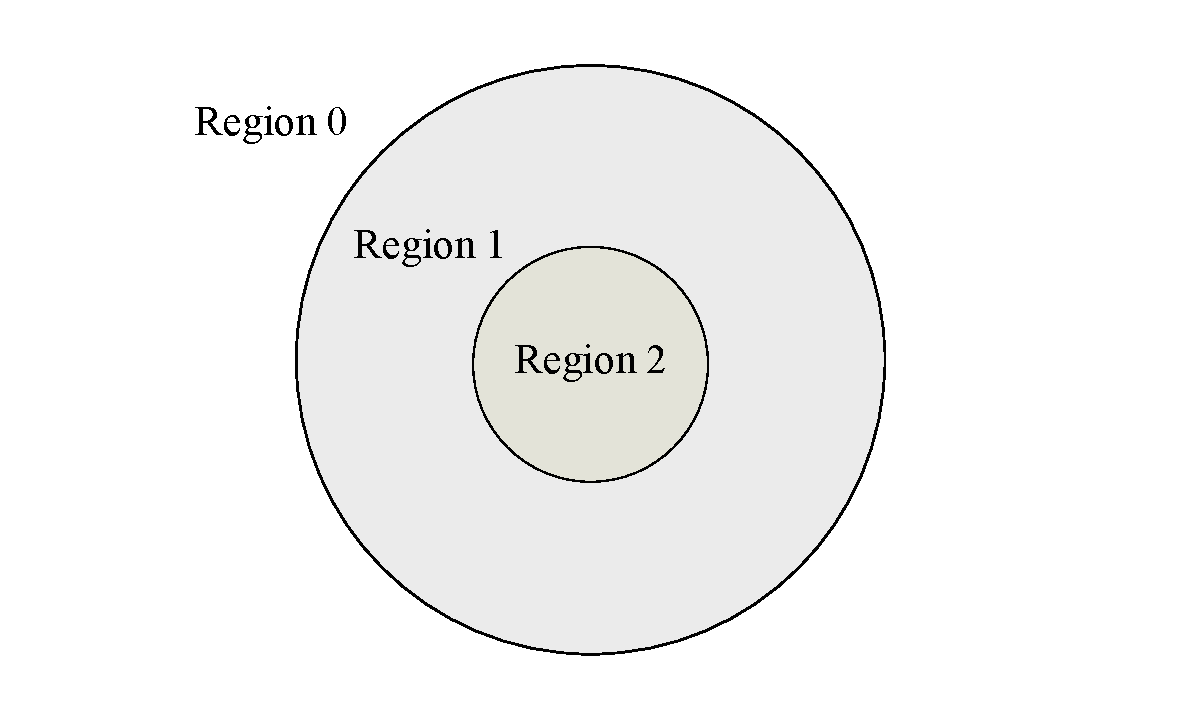
\includegraphics[width=.65\textwidth]{Figures/Region.pdf}
    \caption{Schematic illustration of space division. Computations of electric fields for a specific position is based on the located region.}
    \label{fig:region}
\end{figure*}
\noindent
On the basis of aforementioned MATLAB functions (subroutines), we are now able to construct modules to compute electric fields.
Because dielectric functions are assumed to be piecewise homogeneous, the computation of electric fields can be divided into two (three) concentric-sphere regions, as shown in Figure~\ref{fig:region}.
Hence, we construct calculation modules for each region, i.e., \cfont{EFieldR0}, \cfont{EFieldR1}, and so on.\footnote{For the case of the core/shell sphere, the corresponding modules have not been completely constructed. Therefore, the readers can extend the code to their needs according to this scheme.}
To briefly explain the details, we present the flowchart of the module \cfont{EFieldR0}, as shwon in Fig.~\ref{FC:EFieldR0}.
At the beginning of \cfont{EFieldR0}, we make a series of decisions to check whether the required variables (structure arrays, objects in MATLAB) exist or not.
Processes of checking variables allow us to prevent redundant calculations in a for-loop and compute the needed variables in advance.
Here, \cfont{DRad} and \cfont{ARad} denote the radial functions of the donor and the acceptor individually; \cfont{DNAng} and \cfont{ANAng} denote the normalized angular functions of the donor and the acceptor, repectively.
Also, \cfont{emphi}, \cfont{Source}, and \cfont{Scat}, respresent the normalized azimuthal functions of the acceptor, the expansion coefficients of the dipole source, and the scattering coefficients, respectively.\footnote{Because the code is constructed to calculate the generalized spectral overlap in the resonance energy transfer theory, we use the language of donor and acceptor to name the variables.}
\newpage
\begin{figure}[!h]
    \begin{center}
    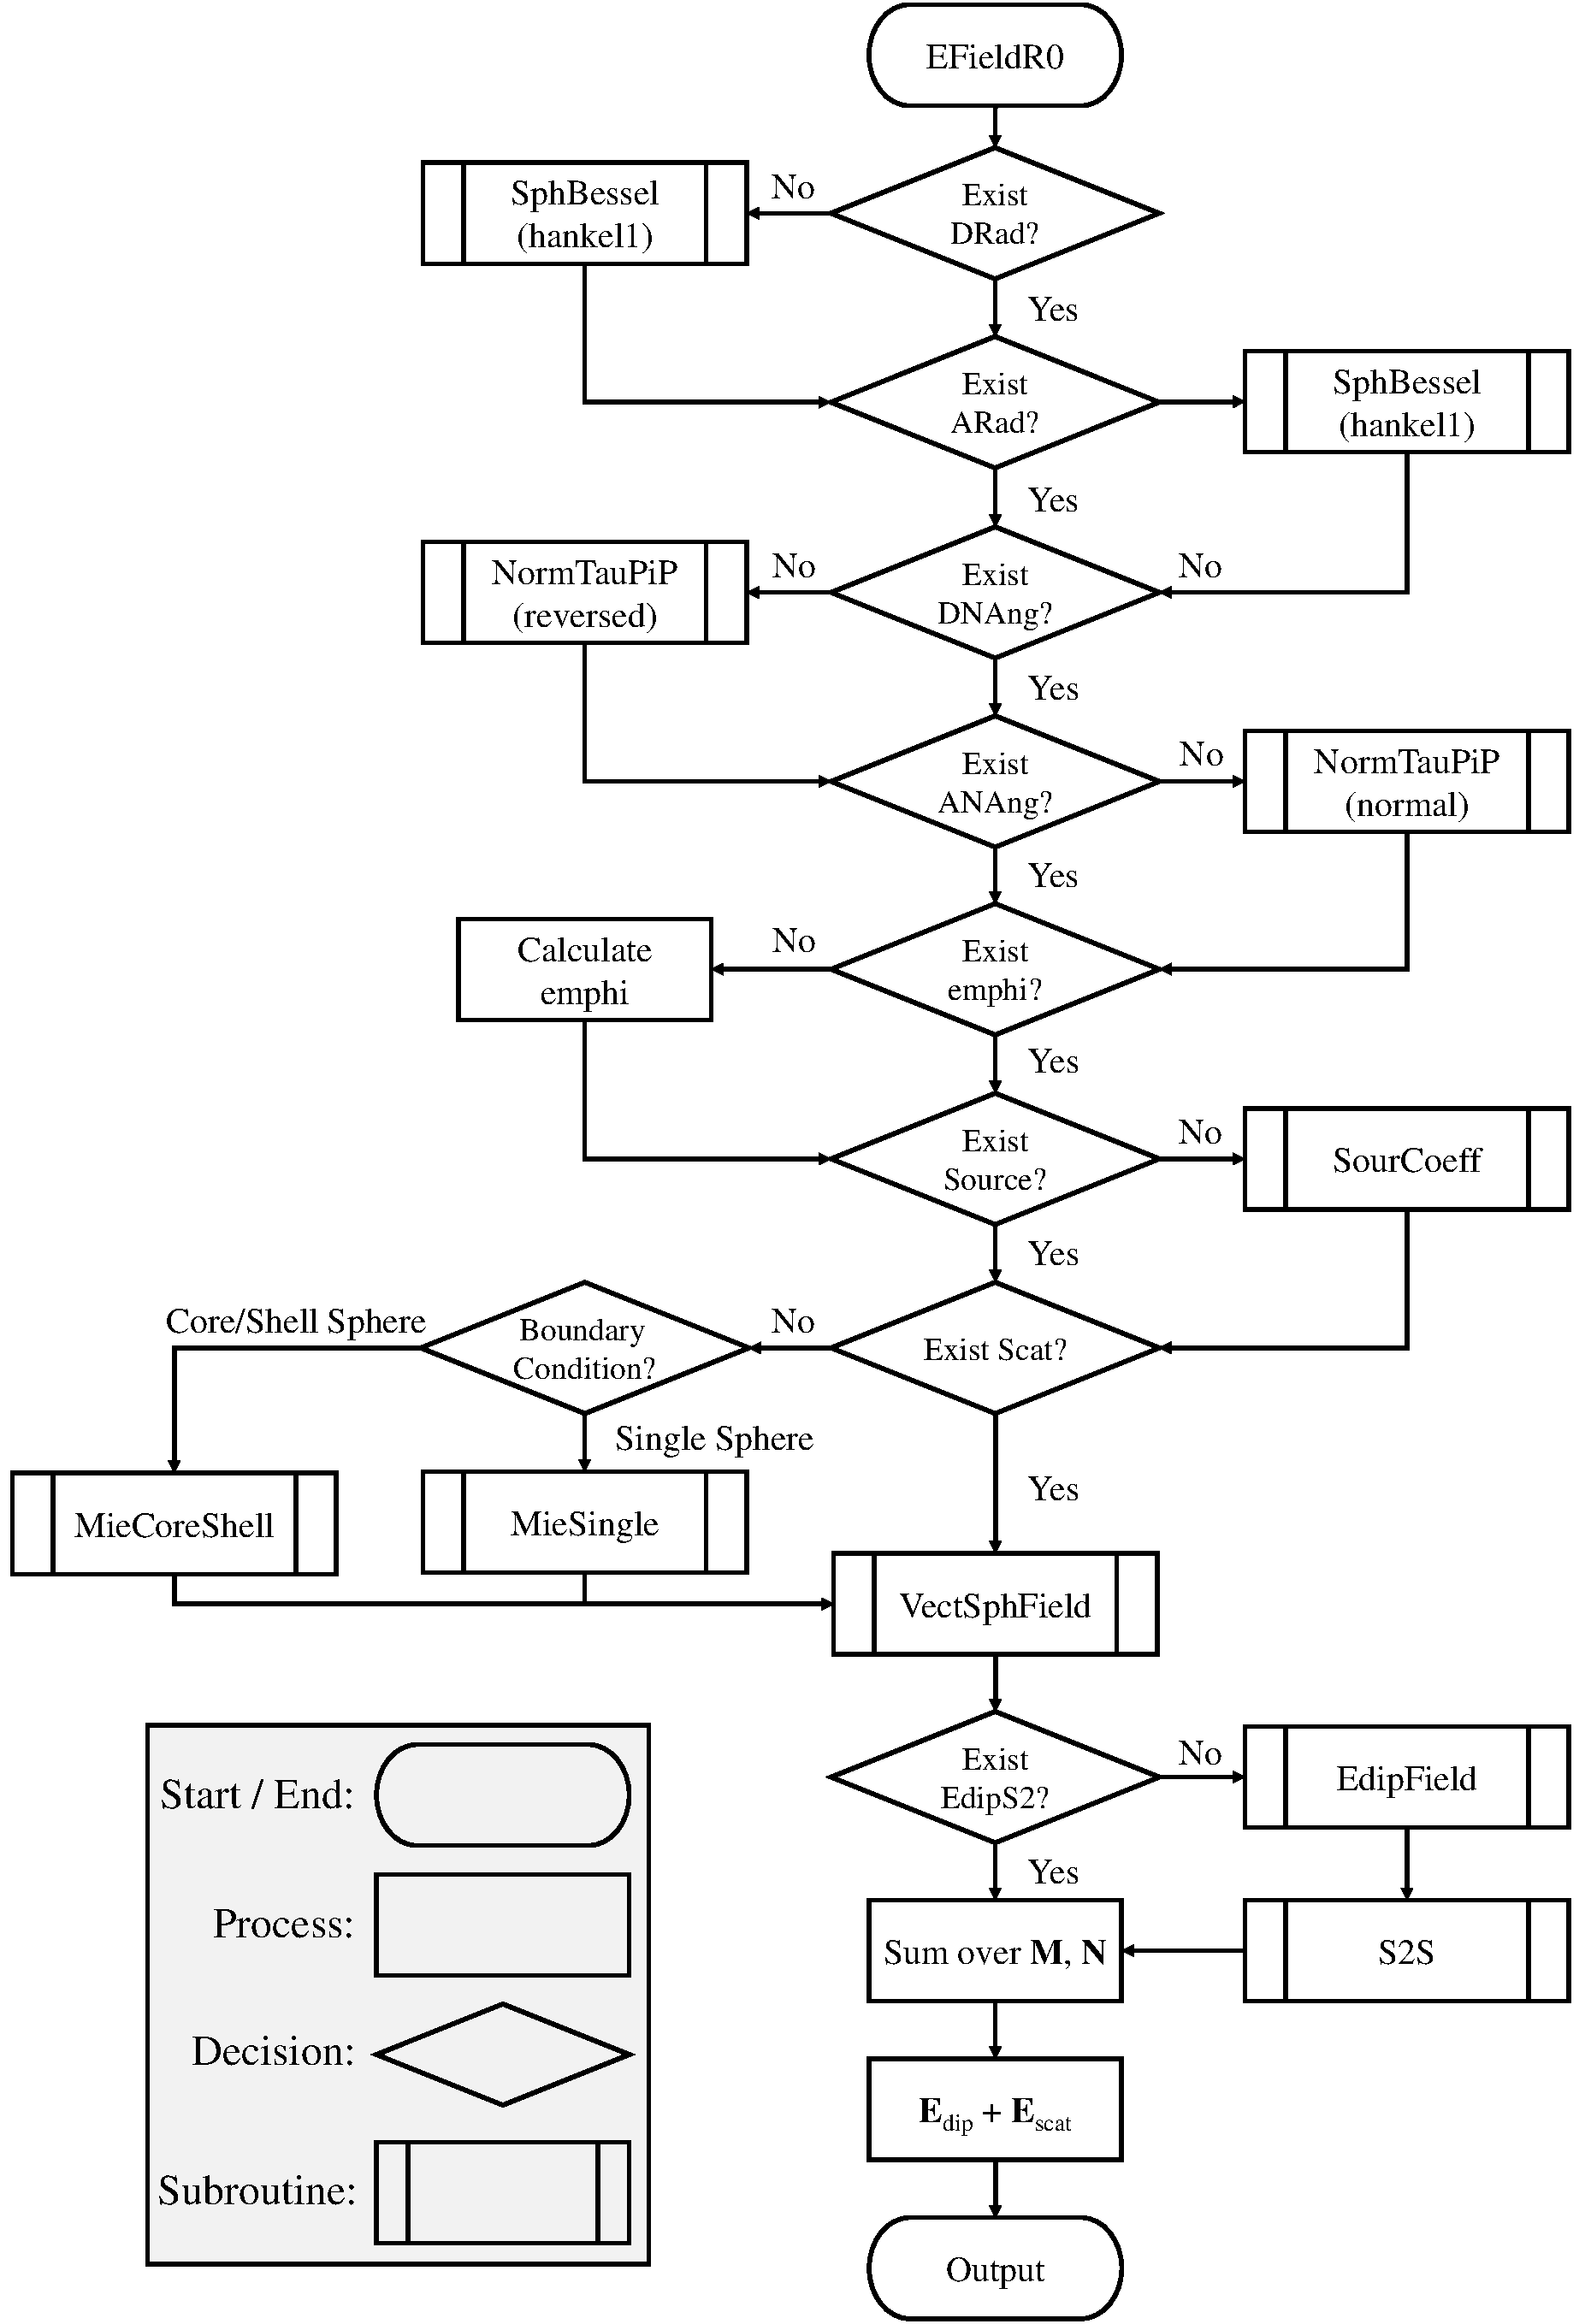
\includegraphics[width=.87\textwidth]{Figures/EFieldR0.pdf}
    \caption{Flowchart of module EFieldR0}
    \label{FC:EFieldR0}
    \end{center}
\end{figure}
\newpage\noindent
If variables have not been calculated, the code will call the corresponding functions to calculate them.
In \cfont{EFieldR0}, an additional step is needed to compute the electric field generated by the electric dipole (in other words, incident electric field) because the dipole is placed in the zeroth region, as shown in the final decision.
Once the variables are prepared, we sum over all the vector spherical functions and the contribution from the electric point dipole ($\vb{E}_\mathrm{dip}$), and output the results.
\blue{Another demonstration module, \cfont{EFieldR1}, can be found in Appendix J.}
\lstinputlisting[caption={Module of calculating electric fields in region 0},captionpos=b,label={F:EfieldR0}]{code/EFieldR0.m}
\newpage
\subsectiontoc{Total Code Structure}
\begin{figure}[!h]
    \begin{center}
    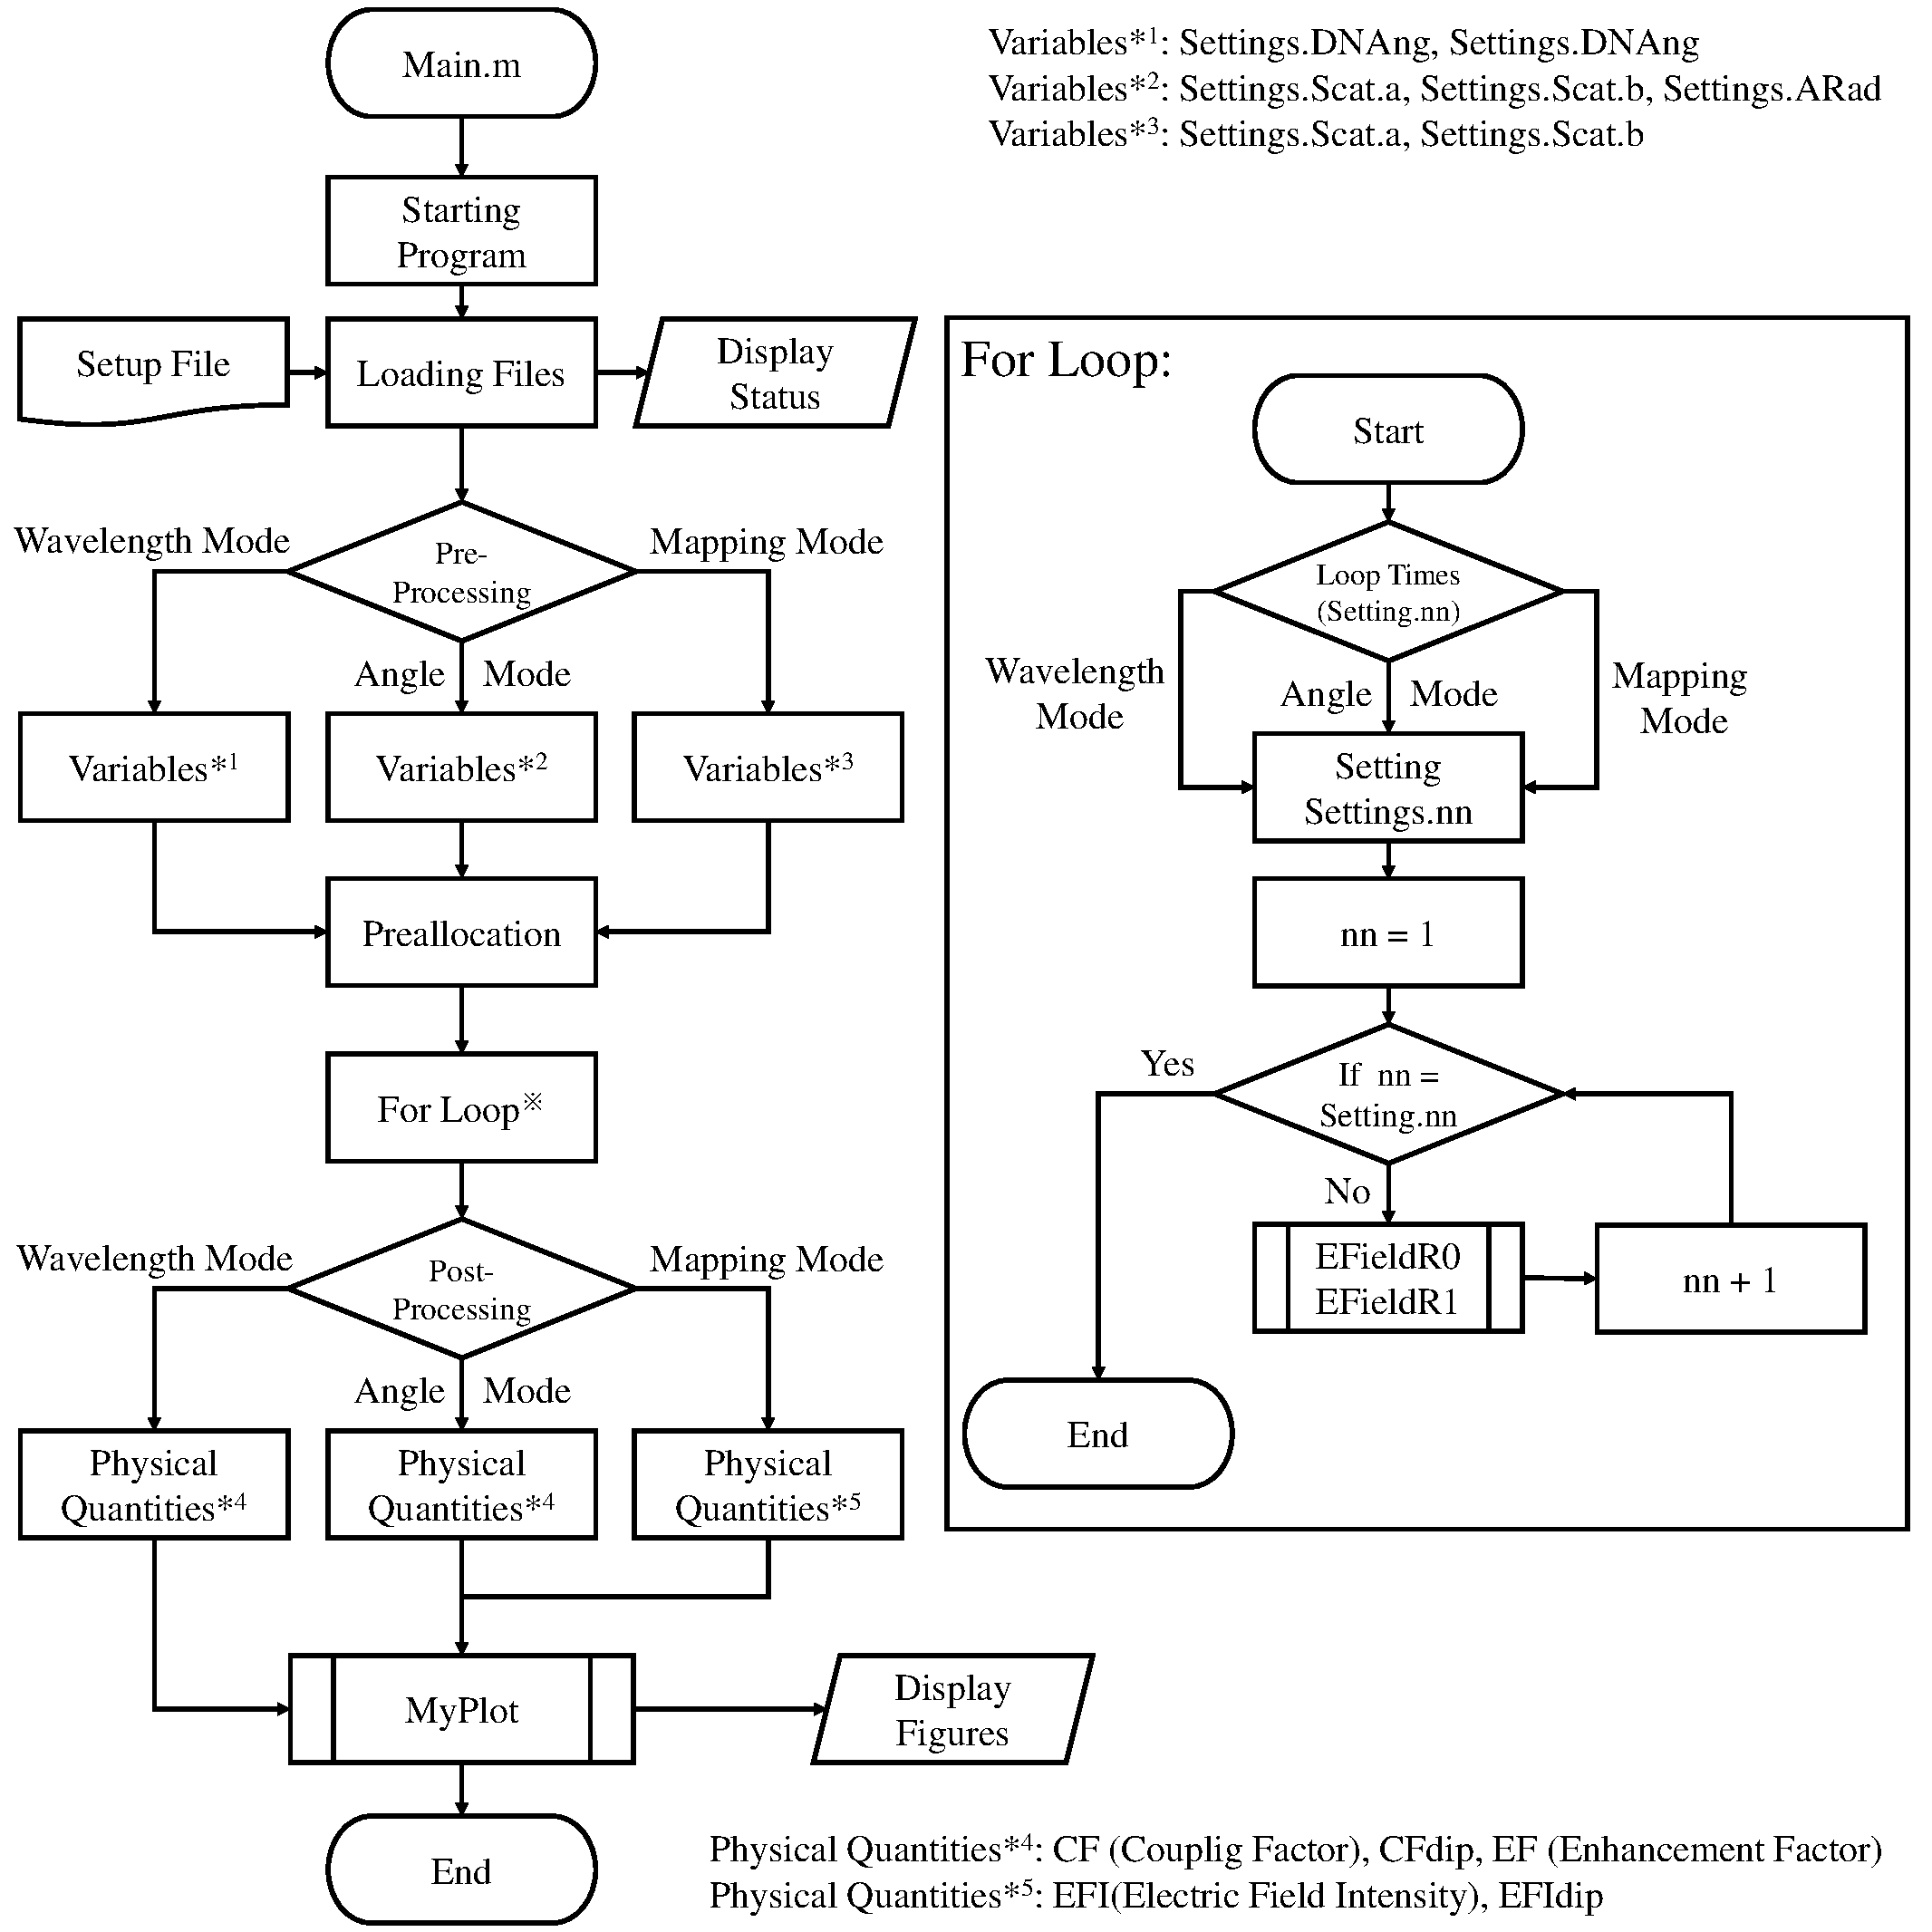
\includegraphics[width=1\textwidth]{Figures/Main.pdf}
    \caption{Computation flowchart of generalized Mie theory}
    \label{FC:Main}
    \end{center}
\end{figure}
\noindent
The calculation of generalized Mie theory is accomplished by \cfont{Main.m}, which performs loading the setup file, selecting the calculation mode, computing physical quantities, and outputting of figures, as shown in Fig.~\ref{FC:Main}.
To initiate the program, we need to input the setting file of calculation details.
The file path and the file name should be filled in line 17 and 18.
In addition, the size of the output figures can be tuned by a dimensionless scaling factor in line 19, in order to prevent the figures from exceeding screen size.
\blue{Also note that non-built-in functions are called in \cfont{main.m} and the source code can be found in Appendix L.}

\begin{center}
    \textrm{MATLAB program for calculating electric fields based on generalized Mie theory}
\end{center}
\vspace{-0.6 cm}
\lstinputlisting{code/Main.m}
\newpage
\subsectiontoc{Setup an Input File}
\noindent
In this subsection, we describe how to construct a setting file to perform a job.
In the current version, \cfont{main.m} supports four calculation modes, including 
wavelength, angle, field mapping, and Purcell factor.
For example, the setting under the wavelength mode is shown at the bottom.
First, we need to assign the position and the orientation of the donor and acceptor dipole in lines 4-15.
Second, the maximum expansion order is given in line 17.
Third, we set the properties of the dielectric environment in lines 19-51, including the type of the scatterer (\cfont{'sphere'} or \cfont{'coreshell'}), the frequency-dependent dielectric functions, and the radius of the scatterer.
In addition, the default output of figures is adjustable in lines 55-62 if the modification is needed.
Finally, the parameters set in lines 4-52 will be packaged to a structure array in lines 68-93.
Setting files for the other modes can be found in \blue{Appendix L}.
\lstinputlisting{code/InputFile/Demo_WavelengthMode.m}


\newpage
\begin{appendix}
\sectiontoc{Appendix}
\subsectiontoc{A. Derivation of Eqs.~(\ref{Eq:InhomoPDEE}) and (\ref{Eq:InhomoPDEH})}
To derive the decoupled differential equation of Maxwell's equations for electric fields, we take a curl on the Faraday's law:
\begin{align}
    \nonumber
    \nabla\times{\nabla\times{\eme(\br,\omega)}} &= i\omega\nabla\times{\emb(\br,\omega)}\\
    \nonumber
    &= i\omega\mu_0\nabla\times{\emh(\br,\omega)}\\
    \nonumber
    &= \omega^2\mu_0\emd(\br,\omega)\\
    \nonumber
    &= \omega^2\mu_0\left[\epsilon_0\epsilon_\textrm{r}(\br,\omega)\eme(\br,\omega) + \emp_\textrm{D}(\br,\omega)\right]\\
    &= \frac{\omega^2}{c^2}\epsilon_\textrm{r}(\br,\omega)\eme(\br,\omega) + \frac{\omega^2}{\epsilon_0c^2}\emp_\textrm{D}(\br,\omega).
    \label{Eq:derPDEE}
\end{align}
Utilizing the vector identity $\nabla\times{\nabla\times{}}=\nabla\nabla\cdot{} -\nabla^2$, the differential equation becomes:
\begin{align}
    %\nonumber
    \left[\frac{\omega^2\epsilon_\textrm{r}(\br,\omega)}{c^2}-\nabla\times{\nabla\times}\right]\eme(\br,\omega)
    =\left[\nabla^2 + \frac{\omega^2\epsilon_\textrm{r}(\br,\omega)}{c^2}\right]\eme(\br,\omega)
    = -\frac{\omega^2}{\epsilon_0c^2}\emp_\textrm{D}(\br,\omega).%\\
    %\Rightarrow\quad&\left[\nabla^2 + k^2(\br,\omega)\right]\eme(\br,\omega)
    %= -\frac{\omega^2}{\epsilon_0c^2}\emp_\textrm{D}(\br,\omega)
\end{align}
Using the same trick on the Maxwell-Amp\`ere equation, we reach the result that
\begin{align}
    \nonumber
    \nabla\times{\nabla\times{\emh(\br,\omega)}} &= -i\omega\nabla\times{\emd(\br,\omega)}\\
    \nonumber
    &= -i\omega\nabla\times{\left[\epsilon_0\epsilon_\textrm{r}(\br,\omega)\eme(\br,\omega) + \emp_\textrm{D}(\br,\omega)\right]}\\
    \nonumber
    &= -i\omega\epsilon_0\nabla\epsilon_\textrm{r}(\br,\omega)\times\eme(\br,\omega)
    -i\omega\epsilon_0\epsilon_\textrm{r}(\br,\omega)\nabla\times{\eme(\br,\omega)}
    -i\omega\nabla\times{\emp_\textrm{D}(\br,\omega)}\\
    &\cong\omega^2\mu_0\epsilon_0\epsilon_\textrm{r}(\br,\omega)\emh(\br,\omega)
    -i\omega\nabla\times{\emp_\textrm{D}(\br,\omega)}.
    \label{Eq:derPDEH}
\end{align}
In Eq.~(\ref{Eq:derPDEH}), we assume that the dielectric function is piecewise-homogeneous for each region. In other words, the dielectric function in $i$-th region is independent of position, $\epsilon_\textrm{r}(\br,\omega) \rightarrow \epsilon_{\textrm{r},i}(\omega)$. Therefore, $\nabla\epsilon_\textrm{r}(\br,\omega)=0$ except for $\br$ at boundary. Similarly, we get another inhomogeneous differential equation for the magnetizing fields in the $i$-th region:
\begin{align}
    \nonumber
    \left[\frac{\omega^2\epsilon_{\textrm{r},i}(\br,\omega)}{c^2}-\nabla\times{\nabla\times}\right]\emh^{(i)}(\br,\omega)
    &=\left[\nabla^2 + \frac{\omega^2\epsilon_{\textrm{r},i}(\br,\omega)}{c^2}\right]\emh^{(i)}(\br,\omega)\\
    &= i\omega\nabla\times{\sum_j\emp_\textrm{D}^{(j)}(\br,\omega)},
\end{align}
where the superscript $(i)$ denotes the $i$-th region.
In the derivation, the requirement of piecewise-homogeneous dielectric function is not necessary to get the result in Eq.~(\ref{Eq:derPDEE}).
For the sake of consistency, we impose the additional condition to dielectric functions, which are presented in the tutorial [Eqs.~(\ref{Eq:InhomoPDEE}) and~(\ref{Eq:InhomoPDEH})].
\newpage
\subsectiontoc{B. Derivation from Eq.~(\ref{Eq:2ODE}) to Eq.~(\ref{Eq:scalarODE})}
Here, we aim to prove that the vector differential equation in Eq.~(\ref{Eq:2ODE}) can be reduced to the scalar differential equation in Eq.~(\ref{Eq:scalarODE}).
To get the result, we need to verify that
\begin{align}
    \left[k_i^2(\omega)-\nabla\times\nabla\times\right]
    \mathcal{T}_{\vb{K}}\left\{\phi^{(i)}(\vb{r},\omega)\right\}=0=
    \mathcal{T}_{\vb{K}}\left\{\left[k_i^2(\omega)+\nabla^2\right]
    \phi^{(i)}(\vb{r},\omega)\right\},
\end{align}
where $\vb{K}=\{\vb{M},\vb{N}\}$. Recall that $\mathcal{T}_{\vb{K}}\left\{\cdot\right\}$ transforms a scalar field to a transverse vector field [definitions can be found in Eq.~(\ref{Eq:TM}) and Eq.~(\ref{Eq:TN})].
The thing we need to do is change the order of differential operators.
From the definition, the differential equation of $\vb{M}^{(i)}(\vb{r},\omega)$ is
\begin{align}
    \left[k_i^2(\omega)-\nabla\times\nabla\times\right]
    \nabla\times\left[\vb{r}\phi^{(i)}(\vb{r},\omega)\right]=0.
\end{align}
It is obvious to obtain that $k_i^2(\omega)\nabla\times\left[\vb{r}\phi^{(i)}(\vb{r},\omega)\right]=\nabla\times\left[\vb{r}k_i^2(\omega)\phi^{(i)}(\vb{r},\omega)\right]$ because the curl operator does not operate on $k_i(\omega).$ Moreover, the triple-curl operator can be simplified to
\begin{align}
    \label{Eq:tricurl1}
    \nabla\times\nabla\times\nabla\times\left[\vb{r}\phi^{(i)}(\vb{r},\omega)\right] &=
    \nabla\times\left\{\nabla\nabla\cdot\left[\vb{r}\phi^{(i)}(\vb{r},\omega)\right]-\nabla^2\left[\vb{r}\phi^{(i)}(\vb{r},\omega)\right]\right\}\\
    \label{Eq:tricurl2}
    &=
    -\nabla\times\nabla^2\left[\vb{r}\phi^{(i)}(\vb{r},\omega)\right]\\
    \label{Eq:tricurl3}
    &=
    -\nabla\times\left[\vb{r}\nabla^2\phi^{(i)}(\vb{r},\omega)+2\nabla\phi^{(i)}(\vb{r},\omega)\right]\\
    \label{Eq:tricurl4}
    &=
    -\nabla\times\left[\vb{r}\nabla^2\phi^{(i)}(\vb{r},\omega)\right].
\end{align}
In the first equation, we use the fact that $\nabla\times\nabla\times=\nabla\nabla\cdot-\nabla^2$.
Also, because the curl of the gradient of any scalar function is identical to zero, only $\nabla\times\nabla^2\left[\vb{r}\phi^{(i)}(\vb{r},\omega)\right]$ contributes a nonzero result.
Finally, it shows that 
\begin{align}
    \left[k_i^2(\omega)-\nabla\times\nabla\times\right]
    \nabla\times\left[\vb{r}\phi^{(i)}(\vb{r},\omega)\right]=
    \nabla\times\left\{\vb{r}\left[k_i^2(\omega)+\nabla^2\right]\phi^{(i)}(\vb{r},\omega)\right\}=0.
\end{align}
The derivation of $\vb{N}^{(i)}(\vb{r},\omega)$ is similar to that of $\vb{M}^{(i)}(\vb{r},\omega)$. Readers can verify themselves.
\newpage
\subsectiontoc{C. Scalar Helmholtz Equation and its Eigenfunctions}
The scalar Helmholtz equation is defined as $\left[\nabla^2+k_i^2\right]\phi^{(i)}(\mathbf{r},\omega)=0$.
Recall that $k_i\equiv\nr_ik_0$ and $k_0=\omega/c$.
Expanding Laplacian operator in the spherical coordinate, we get the equation:
\begin{align}
    \left[\frac{1}{r^2}\p{}{r}\left(r^2\p{}{r}\right) +
    \frac{1}{r^2}\hat{J}^2+
    k_i^2\right]\phi^{(i)}(\mathbf{r},\omega) = 0,
\end{align}
where $\hat{J}^2$ is the angular part of Laplacian, 
\begin{align}
    \hat{J}^2 =
    \frac{1}{\sin\theta}\p{}{\theta}\left(\sin\theta\p{}{\theta}\right) +
    \frac{1}{\sin^2\theta}\frac{\partial^2}{\partial\phi^2},
\end{align}
By using the separation of variables, i.e., $\phi^{(i)}(\mathbf{r},\omega) \sim R^{(i)}(r,\omega)Y(\theta,\phi)$, we divide the differential equation into the radical part
\begin{align}
    &\left[\frac{\diff}{\diff r}\left(r^2\frac{\diff}{\diff{r}}\right) +(k_ir)^2 - n(n+1)\right]R^{(i)}(r,\omega) = 0,
\end{align}
and the angular part $\hat{J}^2Y(\theta,\phi)+n(n+1)Y(\theta,\phi)=0$.
Furthermore, the angular function $Y(\theta,\phi)$ can be separated again to $\Theta(\theta)\Phi(\phi)$ and get the two equations,
\begin{align}
    \label{Eq:DiffPolar}
    &\left[\frac{1}{\sin\theta}\frac{\diff}{\diff\theta}\left(\sin\theta\frac{\diff}{\diff\theta}\right) + n(n+1) - \frac{m^2}{\sin^2\theta}\right]\Theta(\theta) = 0\\
    \label{Eq:DiffAzimuthal}
    &\left(\frac{\diff^2}{\diff\phi^2}+m^2\right)\Phi(\phi) = 0.
\end{align}
The solution of Eq.~(\ref{Eq:DiffAzimuthal}), the azimuthal part, with the boundary condition $\Phi(\phi) = \Phi(\phi+2\pi)$ is 
$\Phi(\phi) = e^{im\phi},~m\in\mathbb{Z}$.
For the polar part [Eq.~(\ref{Eq:DiffPolar})], the solutions are associated Legendre polynomials,
\begin{align}
    \Theta(\theta) = P_n^m(\cos\theta), \qquad n\geq|m|.
\end{align}
Here, associated Legendre polynomials can be defined by Legendre polynomials [$P_n(\cos\theta)$],
\begin{align}
    \label{Eq:alp}
    P_n^m(\cos{\theta}) = (-1)^m\sin^m{\theta}\frac{\diff^m}{\diff(\cos{\theta})^m}P_n(\cos\theta), \qquad m\geq 0.
\end{align}
Because $m\in\mathbb{Z}$, which is requested by the azimuthal differential equation, we need to define associated Legendre polynomials for negative arguments of $m$.
Customarily, we can define them using Rodrigues' formula; however, we do not adopt this scheme due to the redundant computation of normalization.
According to Eq.~(\ref{Eq:DiffPolar}), it is obvious that associated Legendre polynomials do not change when $m\rightarrow-m$.
Intuitively thinking, we can set $P_n^{-m}(\cos\theta)=P_n^m(\cos\theta)$.
However, in practice, we choose the convention in angular momentum theory, which includes the Condon-Shortley phase, $(-1)^m$,
\begin{align}
    P_n^{-m}(\cos\theta) \equiv (-1)^mP_n^m(\cos\theta), \qquad m\geq 0.
\end{align}
The additional phase on associated Legendre polynomials makes Eq.~(\ref{Eq:OpLadd}) hold, i.e.,
\begin{align}
    &\bra{\theta,\phi}\hat{J}_\pm\ket{n,m}=\bra{\theta,\phi}C_\pm(n,m)\ket{n,m\pm1}.%\\
    %\nonumber
    %\Rightarrow
    %&\int\diff{\Omega}'\bra{\theta,\phi}\hat{J}_\pm\ket{\theta',\phi'}\bra{\theta',\phi'}\ket{n,m}=\bra{\theta,\phi}C_\pm(n,m)\ket{n,m\pm1}\\
    %\Rightarrow
    %&e^{\pm i\phi}\left[\pm\p{}{\theta}+i\cot\theta\p{}{\phi}\right]c_{n,m}P_n^{m}(\cos\theta)e^{im\phi}=C_\pm(n,m)c_{n,m\pm1}P_n^{m\pm1}(\cos\theta)e^{i(m\pm1)\phi}
\end{align}
This requirement allows us to compute associated Legendre polynomials via spectral methods, which provides high-precision numerical results when $n$ is large.
As for the radial-part function, the differential equation can be reduced to the well-known spherical Bessel differential equation via the transformation,
\begin{align}
    z(k_ir) = R^{(i)}(r,\omega)\cdot\sqrt{k_ir}.
\end{align}
%Notice that the wavenumber $k$ is a complex number when we consider in absorptive media. ($k = \tilde{n}_\textrm{r}k_\textrm{vac}$, $\tilde{n}_\textrm{r} = n_\textrm{r} + i\kappa_\textrm{r}$)
%$n_\textrm{r}$ is the relative refractive index, and $\kappa_\textrm{r}$ is the extinction coefficient.
The differential equation becomes:
\begin{align}
    \left\{k_ir\cdot\frac{\diff}{\diff (k_ir)}\left[(k_ir)\cdot\frac{\diff }{\diff{(k_ir)}}\right]+\left[(k_ir)^2-\left(n+\frac{1}{2}\right)^2\right]\right\}z(k_ir) = 0,
\end{align}
The function $z(k_ir)$ denotes the independent solutions of the differential equation, spherical Bessel function of the first kind and the second kind, $\{j_n(k_ir),y_n(k_ir)\}$, and the spherical Hankel function of the first kind and the second kind, $\{h_n^{(1)}(k_ir),h_n^{(2)}(k_ir)\}$.
Notice that both of the set are defined in the complex domain since the input variable $k_ir$ may be a complex number.
In addition, the two spherical Hankel functions are defined by the complex linear combination of the two spherical Bessel functions:
\begin{align}
    h_n^{(1)}(\rho) &= j_n(\rho) + iy_n(\rho),\\
    h_n^{(1)}(\rho) &= j_n(\rho) - iy_n(\rho).
\end{align}
\newpage
\subsectiontoc{D. Auxiliary Equations for proving the orthogonality of Vector Spherical Functions}
In the discussion of orthogonality, we encounter the following two integrals with respect to solid angle,
\begin{align}
    &\nonumber
    \int i
    \left[
    \tau_{n'm'}(\theta)\pi_{nm}(\theta)+
    \pi_{n'm'}(\theta)\tau_{nm}(\theta)
    \right]e^{i(m-m')\phi}~\diff\Omega=0\\
    \nonumber
    \\
    &\int \left[
    \tau_{n'm'}(\theta)\tau_{nm}(\theta)+
    \pi_{n'm'}(\theta)\pi_{nm}(\theta)
    \right]e^{i(m-m')\phi}~\diff\Omega
    =n(n+1)f_{nm}\delta_{nn'}\delta_{mm'}.
\end{align}
Here, we are going to prove the two equations.
First, it is easy to obtain that the integral of the azimuthal part returns a Kronecker delta.
In other words, cases for $m'\neq m$ is always identical to zero.
Hence, we only need to consider the polar-part integrals for integrands that $m'=m$.
For integrands of crossing terms of $\tau$ and $\pi$ functions, the polar-part integral becomes
\begin{align}
    \nonumber
    &\int_0^\pi\left[\tau_{n'm}(\theta)\pi_{nm}(\theta)+
    \pi_{n'm}(\theta)\tau_{nm}(\theta)\right]\sin\theta\diff\theta\\
    \label{Eq:Appendixtppt1}
    &=m\int_0^\pi \left[P_n^m(\cos\theta)\frac{\diff P_{n'}^m(\cos\theta)}{\diff\theta}+
    P_{n'}^m(\cos\theta)\frac{\diff P_n^m(\cos\theta)}{\diff\theta}\right]\diff{\theta}\\
    \label{Eq:Appendixtppt2}
    &=\left.m P_n^m(\cos\theta)P_{n'}^m(\cos\theta)\right|_0^\pi=0
\end{align}
In Eq.~(\ref{Eq:Appendixtppt1}), we apply the definitions of $\tau$ and $\pi$ functions.
Using the chain rule and the fundamental theorem of calculus, we obtain the result in Eq.~(\ref{Eq:Appendixtppt2}).
Equation (\ref{Eq:Appendixtppt2}) is equivalent to zero because $P_n^m(-1)=0=P_n^m(1)$ except for $m=0$.
For the case of $m=0$, the equation still equals zero because the associated Legendre polynomials are multiplied by $m$ beforehand.
For the integrands of the summation of $\tau$-square and $\pi$-square we use the identity,
\begin{align}
    \nonumber
    2\sin\theta\left[\tau_{n'm'}(\theta)\tau_{nm}(\theta)+
    \pi_{n'm'}(\theta)\pi_{nm}(\theta)\right]
    =&
    2\sin\theta\left[
    \frac{\diff P_{n'}^m}{\diff\theta}
    \frac{\diff P_{n}^m}{\diff\theta}
    +m^2\frac{P_{n'}^m}{\sin\theta}\frac{P_n^m}{\sin\theta}
    \right]\\
    \nonumber
    =&
    2\sin\theta~n(n+1)P_{n'}^mP_n^m\\
    &+
    \frac{\diff}{\diff\theta}\left[
    \sin\theta~P_{n'}^m~\frac{\diff P_{n}^m}{\diff\theta}+
    \sin\theta~P_{n}^m~\frac{\diff P_{n'}^m}{\diff\theta}
    \right],
    \label{Eq:Appendixttpp}
\end{align}
which makes the integral become
\begin{align}
    \nonumber
    &\int\left[
    \tau_{n'm'}(\theta)\tau_{nm}(\theta)+
    \pi_{n'm'}(\theta)\pi_{nm}(\theta)
    \right]e^{i(m-m')\phi}~\diff\Omega\\
    &=n(n+1)\int_0^{\pi}
    P_{n'}^m(\cos\theta)P_n^m(\cos\theta)\sin\theta\diff\theta
    \int_0^{2\pi} e^{i(m-m')\phi}~\diff\phi=
    n(n+1)f_{nm}\delta_{nn'}\delta_{mm'}.
\end{align}
Note that Eq.~(\ref{Eq:Appendixttpp}) can be derived from the definition of associated Legendre differential equation, as depicted in Eq.~(\ref{Eq:DiffPolar}).
\newpage
\subsectiontoc{E. Expansion of Dyadic Delta Function in a Spherical Coordinate}
According to the orthogonality of (partially) normalized vector spherical functions,
$\norF{L}_{nm}^{(\RomanI)}$, $\norF{M}_{nm}^{(\RomanI)}$, and $\norF{N}_{nm}^{(\RomanI)}$,
the normalized vector spherical functions form a complete basis.
Thus, a dyadic delta function can be expanded as follows,
\begin{align}
    \nonumber
    \tensori\delta(\vb{r}-\vb{r'})=\int_0^\infty k^2\mathrm{d}k
    &\sum_{nm}\left[\vphantom{\frac{a}{b}}
    \norF{L}_{nm}^{(\RomanI)}(kr,\theta,\phi)\otimes\norF{A}_{nm}(kr',\theta',\phi')\right.\\
    \nonumber
    &\hspace{0.4cm}+\left.
    \norF{M}_{nm}^{(\RomanI)}(kr,\theta,\phi)\otimes\norF{B}_{nm}(kr',\theta',\phi')\right.\\
    &\hspace{0.4cm}+\left.
    \norF{N}_{nm}^{(\RomanI)}(kr,\theta,\phi)\otimes\norF{C}_{nm}(kr',\theta',\phi')
    \vphantom{\frac{a}{b}}\right].
\end{align}
To solve the unknown vector fields: $\norF{A}_{nm}(kr',\theta',\phi')$, $\norF{B}_{nm}(kr',\theta',\phi')$, and $\norF{C}_{nm}(kr',\theta',\phi')$, we evaluate the following integrals:
\begin{align}
    \mathrm{LHS}_{(\vb{A})}=&\int\mathrm{d}^3\vb{r}~(-1)^{m'}\norF{L}_{n'(-m)'}^{(\RomanI)}(k'r,\theta,\phi)\cdot\tensori\delta(\vb{r-r'})=
    (-1)^{m'}\norF{L}_{n'(-m)'}^{(\RomanI)}(k'r',\theta',\phi')\\
    \nonumber
    \mathrm{RHS}_{(\vb{A})}=&\int\mathrm{d}^3\vb{r}\int_0^\infty k^2\mathrm{d}k \sum_{nm}~
    (-1)^{m'}\norF{L}_{n'(-m)'}^{(\RomanI)}(k'r,\theta,\phi)\cdot
    \norF{L}_{nm}^{(\RomanI)}(kr,\theta,\phi)
    \otimes\norF{A}_{nm}(kr',\theta',\phi')\\
    \nonumber
    =&\int_0^\infty k^2\mathrm{d}k~
    \norF{A}_{nm}(kr',\theta',\phi')\cdot \frac{\pi\delta(k-k')}{2k^2}\delta_{nn'}\delta_{mm'}\\
    =&\frac{\pi}{2}~\norF{A}_{n'm'}(k'r',\theta',\phi')
\end{align}
According to the integral above, we get the relation,
\begin{align}
    \norF{A}_{nm}(kr',\theta',\phi') = \frac{2}{\pi}~(-1)^{m}\norF{L}_{n(-m)}^{(\RomanI)}(kr',\theta',\phi').
\end{align}
In the same way, the unknown vector fields, $\norF{B}_{nm}(kr',\theta',\phi')$, and $\norF{C}_{nm}(kr',\theta',\phi')$, are
\begin{align}
    \norF{B}_{nm}(kr',\theta',\phi') &= \frac{2}{\pi}~(-1)^{m}\norF{M}_{n(-m)}^{(\RomanI)}(kr',\theta',\phi'),\\
    \norF{C}_{nm}(kr',\theta',\phi') &= \frac{2}{\pi}~(-1)^{m}\norF{N}_{n(-m)}^{(\RomanI)}(kr',\theta',\phi').
\end{align}
Finally, the expansion of a dyadic delta function in a spherical coordinate becomes
\begin{align}
    \nonumber
    \tensori\delta(\vb{r}-\vb{r'})=\frac{2}{\pi}\int_0^\infty k^2\mathrm{d}k
    \sum_{nm}(-1)^m
    &\left[\vphantom{\frac{a^2}{b^2}}\right. \hspace{.268cm}
    \norF{L}_{nm}^{(\RomanI)}(kr,\theta,\phi) \otimes
    \norF{L}_{n(-m)}^{(\RomanI)}(kr',\theta',\phi')\\
    \nonumber
    &+\norF{M}_{nm}^{(\RomanI)}(kr,\theta,\phi) \otimes
    \norF{M}_{n(-m)}^{(\RomanI)}(kr',\theta',\phi')\\
    &+\hspace{.08cm}\norF{N}_{nm}^{(\RomanI)}(kr,\theta,\phi) \otimes
    \norF{N}_{n(-m)}^{(\RomanI)}(kr',\theta',\phi')
    \hspace{.1cm}\left.\vphantom{\frac{a^2}{b^2}}\right].
\end{align}
\newpage

\subsectiontoc{F. Contour Integrals in the Free-Space Dyadic Green's Function}
In discussing the spherical expansion of dyadic Green's functions, we need to cope with integrals associated with spherical Bessel functions.
Here, we provide a complete derivation of these integrals.
We start from the integral associated with $\norF{M}_{nm}^{(\RomanI)}(kr,\theta,\phi)$ [Eq.~(\ref{Eq:ContourIntM})],
\begin{align}
    \nonumber
    &\int_0^\infty \frac{k^2}{k^2-k_0^2}
    j_n(kr')j_n(kr)~\diff{k}\\
    \nonumber
    &\quad=
    \frac{1}{2}\int_0^\infty \frac{k^2}{k^2-k_0^2}
    \left[
    h_n^{(1)}(kr')+h_n^{(2)}(kr')
    \right]j_n(kr)~\diff{k}\\
    \nonumber
    &\quad=
    \frac{1}{2}\left[
    \int_0^\infty \frac{k^2}{k^2-k_0^2}
    h_n^{(1)}(kr')j_n(kr)~\diff{k}-
    \int_0^{-\infty} \frac{k^2}{k^2-k_0^2}
    h_n^{(1)}(kr')j_n(kr)~\diff{k}
    \right]\\
    &\quad=
    \frac{1}{2}
    \int_{-\infty}^\infty \frac{k^2}{k^2-k_0^2}
    h_n^{(1)}(kr')j_n(kr)~\diff{k},
\end{align}
where we apply the identities, $j_n(kr')=h_n^{(1)}(kr')+h_n^{(2)}(kr')$ and $h_n^{(2)}(-kr')=(-1)^nh_n^{(1)}(kr')$, to change the interval of the second integral. 
Next, we use contour integration to calculate the integral.
We set the whole close path to be the real axis plus a semicircular path at $k\rightarrow\infty$ in the upper half-plane [Fig.~\ref{Contour} (a)],
\begin{align}
    \nonumber&
    \int_{-\infty}^\infty \frac{k^2}{k^2-k_0^2}h_n^{(1)}(kr')j_n(kr)
    ~\diff{k}\\
    \nonumber
    &\quad=
    \lim_{\epsilon\rightarrow0^+}
    \int_{-\infty}^\infty \frac{k^2h_n^{(1)}(kr')j_n(kr)
    }{(k+k_0+i\epsilon)(k-k_0-i\epsilon)}~\diff{k}\\
    &\quad=
    \lim_{\epsilon\rightarrow0^+}\left[\oint_C \frac{\tilde{k}^2
    h_n^{(1)}(\tilde{k}r')j_n(\tilde{k}r)~\diff{\tilde{k}}}
    {(\tilde{k}+k_0+i\epsilon)(\tilde{k}-k_0-i\epsilon)}
    -
    \lim_{k\rightarrow\infty}\int_0^\pi \frac{\tilde{k}^2
    h_n^{(1)}(\tilde{k}r')j_n(\tilde{k}r)~i\tilde{k}\diff{\theta}}
    {(\tilde{k}+k_0+i\epsilon)(\tilde{k}-k_0-i\epsilon)}\right],
    \label{Eq:AppendContourIntM}
\end{align}
where $\tilde{k}=ke^{i\theta}$ and $\epsilon$ denotes an infinitesimal dissipation.
According to the residue theorem, the contour integral of path $C_1$ becomes
\begin{align}
    \nonumber
    \lim_{\epsilon\rightarrow 0^+}\oint_{C_1} \frac{\tilde{k}^2
    h_n^{(1)}(\tilde{k}r')j_n(\tilde{k}r)~\diff{\tilde{k}}}
    {(\tilde{k}+k_0+i\epsilon)(\tilde{k}-k_0-i\epsilon)}
    &=\lim_{\epsilon\rightarrow 0^+}2\pi i\cdot\mathrm{Res}\left[
    \frac{\tilde{k}^2
    h_n^{(1)}(\tilde{k}r')j_n(\tilde{k}r)}
    {(\tilde{k}+k_0+i\epsilon)(\tilde{k}-k_0-i\epsilon)}
    ,k_0+i\epsilon\right]\\
    &=\pi ik_0
    h_n^{(1)}(k_0r')j_n(k_0r)
\end{align}
\begin{figure*}[!ht]
    \begin{center}
    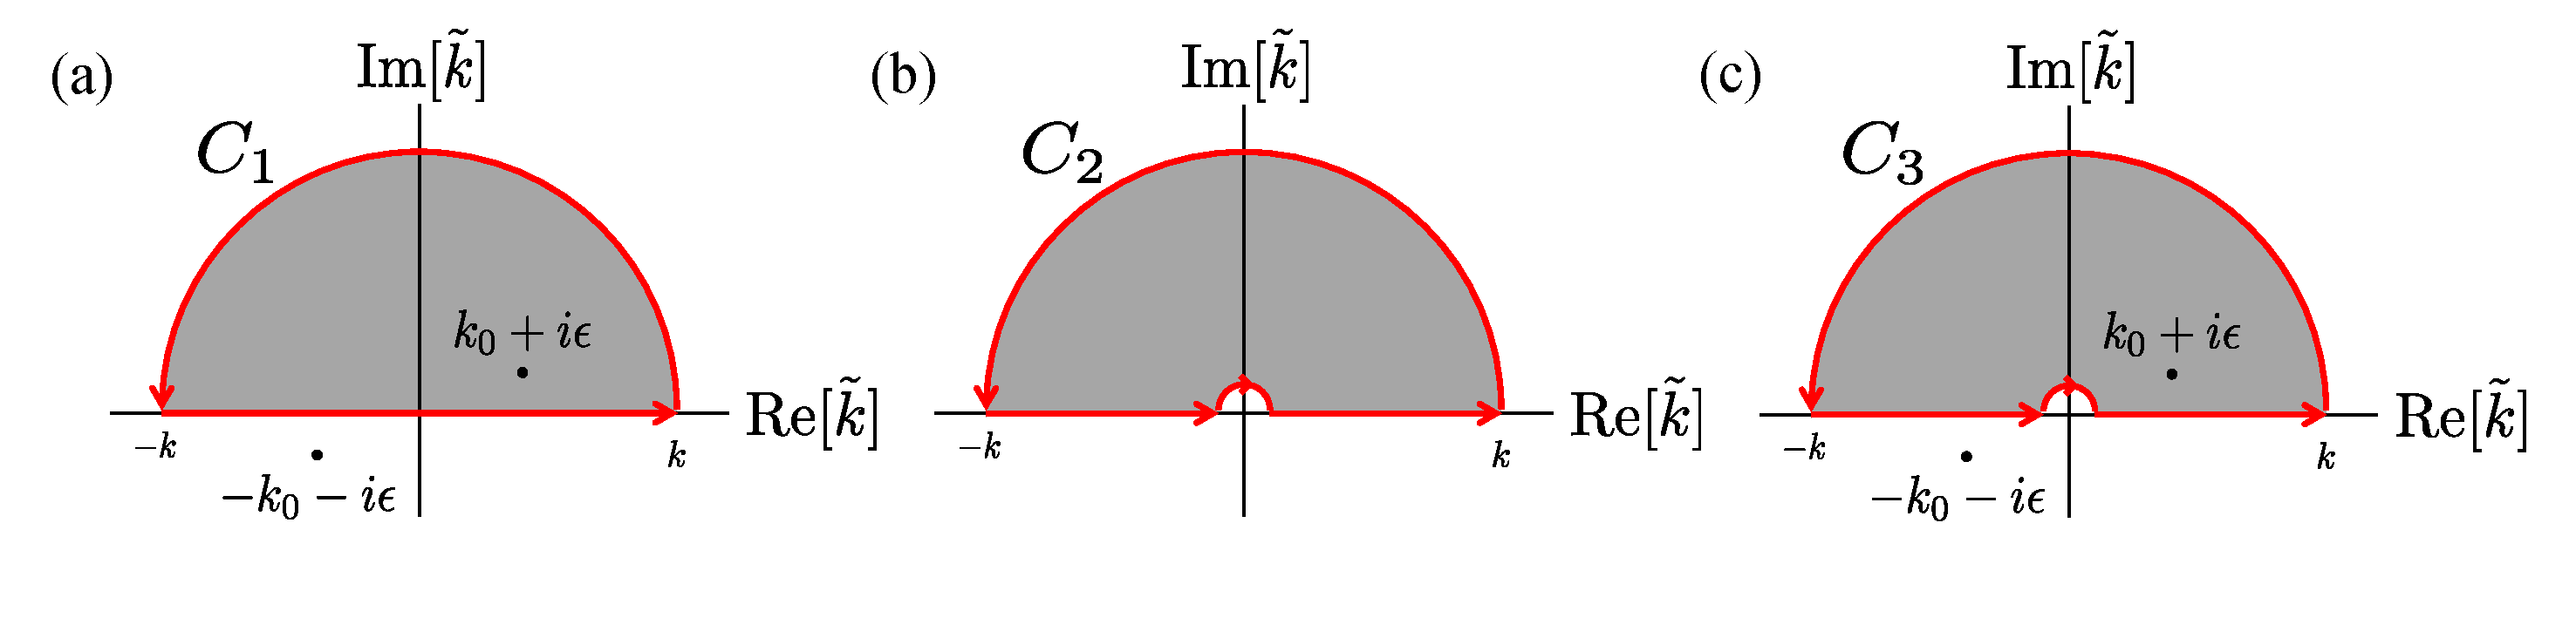
\includegraphics[width=1\textwidth]{Figures/LMNcontour.pdf}
    \caption{The paths of contour integrals in (a) Eq.~(\ref{Eq:AppendContourIntM}), (b) Eq.~(\ref{Eq:AppendContourIntL}), and (c)
    Eq.~(\ref{Eq:AppendContourIntN})}
    \label{Contour}
    \end{center}
\end{figure*}

\noindent
According to the asymptotic expressions of spherical Bessel (Hankel) functions, $j_n(\tilde{k}r)\sim[e^{i(\tilde{k}r-n\pi/2)}-e^{-i(\tilde{k}r-n\pi/2)}]/(2i\tilde{k}r)$ and $h_n^{(1)}(\tilde{k}r')\sim e^{i\tilde{k}r'}/(i^{n+1}\tilde{k}r')$, the integral of semicircular path in the upper half-plane becomes
\begin{align}
    \nonumber
    \lim_{\epsilon\rightarrow0^+}\lim_{k\rightarrow\infty}\int_0^\pi \frac{\tilde{k}^2h_n^{(1)}(\tilde{k}r')
    j_n(\tilde{k}r)~i\tilde{k}\diff{\theta}}
    {(\tilde{k}+k_0+i\epsilon)(\tilde{k}-k_0-i\epsilon)}
    &=\lim_{\epsilon\rightarrow0^+}
    \lim_{k\rightarrow\infty}\int_0^\pi \frac{
    \tilde{k}\left[e^{i\tilde{k}(r'+r)-in\pi/2}-e^{i\tilde{k}(r'-r)+in\pi/2}\right]
    ~\diff{\theta}}
    {i^{-n-1}2rr'(\tilde{k}+k_0+i\epsilon)(\tilde{k}-k_0-i\epsilon)}\\
    &=0,\qquad r<r'.
\end{align}
Moreover, by using Jordan's lemma, if $r<r'$, the integral along the semicircular path in the upper half-plane becomes zero as $k\rightarrow\infty$.
Hence, we get the result
\begin{align}
    \nonumber
    \int_0^\infty \frac{k^2}{k^2-k_0^2}
    j_n(kr')j_n(kr)~\diff{k}
    &=
    \frac{1}{2}\int_{-\infty}^\infty \frac{k^2}{k^2-k_0^2}
    h_n^{(1)}(kr')j_n(kr)~\diff{k}\\
    &=
    \frac{\pi}{2}\cdot ik_0h_n^{(1)}(k_0r')j_n(k_0r),
    \qquad r<r'.
\end{align}
To evaluate the behavior in the region $r>r'$, we can use the same trick to replace $j_n(kr)$ by $[h_n^{(1)}(kr)+h_n^{(1)}(kr)]/2$ and do the same operation described above.
Finally, we get the equation,
\begin{align}
    \int_0^\infty \frac{k^2}{k^2-k_0^2}
    j_n(kr)j_n(kr')~\diff{k}
    &=
    \frac{\pi}{2}\cdot ik_0h_n^{(1)}(k_0r_>)j_n(k_0r_<),
\end{align}
where $r_>=\max(\br,\br')$ and $r_<=\min(\br,\br')$.
Second, we evaluate the integral in Eq.~(\ref{Eq:ContourIntL}) which is associated with $\norF{L}_{nm}^{(\RomanI)}(kr,\theta,\phi)$,
\begin{align}
    \nonumber
    \int_0^\infty
    j_n(kr')j_n(kr)~ \diff{k}
    &=
    \frac{1}{2}\int_0^\infty 
    \left[h_n^{(1)}(kr')+h_n^{(2)}(kr')\right]
    j_n(kr)
    ~\diff{k}\\
    \nonumber
    &=
    \frac{1}{2}\lim_{\delta\rightarrow0}\left[
    \int_\delta^\infty 
    h_n^{(1)}(kr')j_n(kr)
    ~\diff{k}-
    \int_{-\delta}^{-\infty} 
    h_n^{(1)}(kr')j_n(kr)
    ~\diff{k}
    \right]\\
    &=
    \frac{1}{2}\mathrm{PV}
    \int_{-\infty}^\infty
    h_n^{(1)}(kr')j_n(kr)~\diff{k}.
\end{align}
The integral is defined by the Cauchy principal value because a pole exists at $k=0$.
The pole can be identified by the asymptotic expansion of spherical Bessel (Hankel) functions,
\begin{align}
    h_n^{(1)}(kr')j_n(kr)\sim 
    \frac{(2n-1)!!}{i(kr')^{n+1}}
    \frac{(kr)^n}{(2n+1)!!}
    =\frac{1}{ik(2n+1)}
    \frac{r^n}{(r')^{n+1}},\qquad k\rightarrow0.
\end{align}
To calculate the integral, we evaluate a contour integral along the path illustrated in Fig.~\ref{Contour} (b), where an infinitesimally-semicircular path is to bypass the pole.
\begin{align}
    \nonumber
    \mathrm{PV}
    \int_{-\infty}^\infty 
    h_n^{(1)}(kr')j_n(kr)~\diff{k}
    &=
    \oint_C 
    h_n^{(1)}(\tilde{k}r')
    j_n(\tilde{k}r)~\diff{\tilde{k}}\\
    \nonumber
    &-
    \lim_{k\rightarrow\infty}\int_0^\pi 
    h_n^{(1)}(\tilde{k}r')j_n(\tilde{k}r)
    ~i\tilde{k}\diff{\theta}-
    \lim_{k\rightarrow0}\int_\pi^0 
    h_n^{(1)}(\tilde{k}r')j_n(\tilde{k}r)
    ~i\tilde{k}\diff{\theta}\\
    &=\lim_{k\rightarrow0}\int_0^\pi 
    h_n^{(1)}(\tilde{k}r')j_n(\tilde{k}r)
    ~i\tilde{k}\diff{\theta}.
    \label{Eq:AppendContourIntL}
\end{align}
For the same reason (Jordan's lemma), the integral along the semicircular path at $k\rightarrow\infty$ is zero when $r<r'$.
In addition, because the integrand is analytic in the upper half-plane, the Cauchy principal value can be evaluated by the integral of infinitesimally semicircular path, as shown in Eq.~(\ref{Eq:AppendContourIntL}).
According to the integral,
\begin{align}
    \lim_{k\rightarrow0}\int_0^\pi 
    h_n^{(1)}(\tilde{k}r')j_n(\tilde{k}r)
    ~i\tilde{k}\diff{\theta}
    =
    \lim_{k\rightarrow0}\int_0^\pi \frac{1}{i\tilde{k}(2n+1)}
    \frac{r^n}{(r')^{n+1}}~i\tilde{k}\diff{\theta}
    =\frac{\pi}{(2n+1)}
    \frac{r^n}{(r')^{n+1}},
\end{align}
we derive the closed-form expression for general cases (the same technique described former),
\begin{align}
    \int_0^\infty j_n(kr')j_n(kr)\diff{k}&=
    \frac{1}{2}\mathrm{PV}\int_{-\infty}^{\infty}
    h_n^{(1)}(kr')j_n(kr)
    =\frac{\pi}{2(2n+1)}
    \frac{r_<^n}{r_>^{n+1}}.
\end{align}
The last integral, which is associated with $\norF{N}_{nm}^{(\RomanI)}(kr,\theta,\phi)$, can be described by the Cauchy principal value,
\begin{align}
    \label{Eq:targetN}
    \int_0^\infty
    \frac{j_n(kr')j_n(kr)}{k^2-k_0^2}~ \diff{k}
    &=
    \frac{1}{2}\mathrm{PV}
    \int_{-\infty}^\infty 
    \frac{h_n^{(1)}(kr')j_n(kr)}{k^2-k_0^2}~\diff{k}.
\end{align}
We choose the path the same as the second integral to evaluate this Cauchy principal value; however, the integrand is no longer analytic in the upper half-plane because we add an infinitesimal imaginary part to $k_0$ to bypass the poles on the real line.
\begin{align}
    \nonumber
    \mathrm{PV}
    \int_{-\infty}^\infty
    \frac{h_n^{(1)}(kr')j_n(kr)}{k^2-k_0^2}~\diff{k}
    &=
    \lim_{\epsilon\rightarrow0}\oint_C 
    \frac{h_n^{(1)}(\tilde{k}r')j_n(\tilde{k}r)}
    {(\tilde{k}-k_0-i\epsilon)(\tilde{k}+k_0+i\epsilon)}
    ~\diff{\tilde{k}}\\
    \nonumber
    &-
    \lim_{\epsilon\rightarrow0}
    \lim_{k\rightarrow\infty}\int_0^\pi
    \frac{h_n^{(1)}(\tilde{k}r')j_n(\tilde{k}r)}
    {(\tilde{k}-k_0-i\epsilon)(\tilde{k}+k_0+i\epsilon)}~i\tilde{k}\diff{\theta}\\
    &-
    \lim_{\epsilon\rightarrow0}
    \lim_{k\rightarrow0}\int_\pi^0
    \frac{h_n^{(1)}(\tilde{k}r')j_n(\tilde{k}r)}
    {(\tilde{k}-k_0-i\epsilon)(\tilde{k}+k_0+i\epsilon)}
    ~i\tilde{k}\diff{\theta}.
    \label{Eq:AppendContourIntN}
\end{align}
According to the residue theorem, the closed path contour integral becomes
\begin{align}
    \lim_{\epsilon\rightarrow0}\oint_C \frac{
    h_n^{(1)}(\tilde{k}r')j_n(\tilde{k}r)~\diff{\tilde{k}}}
    {(\tilde{k}+k_0+i\epsilon)(\tilde{k}-k_0-i\epsilon)}
    &=\frac{\pi i}{k_0}
    h_n^{(1)}(k_0r')j_n(k_0r)
\end{align}
In addition, the integral along the infinitesimal semicircular path becomes
\begin{align}
    \lim_{\epsilon\rightarrow0}
    \lim_{k\rightarrow0}\int_\pi^0
    \frac{h_n^{(1)}(\tilde{k}r')j_n(\tilde{k}r)}
    {(\tilde{k}-k_0-i\epsilon)(\tilde{k}+k_0+i\epsilon)}
    ~i\tilde{k}\diff{\theta}
    &=
    \frac{\pi}{k_0^2(2n+1)}
    \frac{r^n}{(r')^{n+1}}.
\end{align}
Again, the integral along the semicircular path at $k\rightarrow\infty$ becomes zero.
Eventually, the closed-form expression of Eq.~(\ref{Eq:AppendContourIntN}) is 
\begin{align}
    \mathrm{PV}
    \int_{-\infty}^\infty
    \frac{h_n^{(1)}(kr')j_n(kr)}{k^2-k_0^2}~\diff{k}
    &=\frac{\pi i}{k_0}h_n^{(1)}(k_0r')j_n(k_0r)-
    \frac{\pi}{k_0^2(2n+1)}\frac{r^n}{(r')^{n+1}},
\end{align}
and the target integral in Eq.~(\ref{Eq:targetN}) becomes \begin{align}
    \int_0^\infty
    \frac{j_n(kr')j_n(kr)}{k^2-k_0^2}~ \diff{k}
    &
    =\frac{\pi i}{2k_0}h_n^{(1)}(k_0r')j_n(k_0r)-
    \frac{\pi}{2k_0^2(2n+1)}\frac{r^n}{(r')^{n+1}}.
\end{align}
\newpage
\subsectiontoc{G. Limit of Vector Spherical Functions}
From the definition, the vector spherical functions read
\begin{align}
    \nonumber
    \norF{M}_{nm}^{(\RomanI)} (k_ir,\theta,\phi)
    &= \frac{1}{\sqrt{n(n+1)f_{nm}}}j_n(k_ir)e^{im\phi}\left[ i\pi_{nm}(\theta)\hat{\theta}-\tau_{nm}(\theta)\hat{\phi} \right],\\
    \nonumber
    \norF{N}_{nm}^{(\RomanI)} (k_ir,\theta,\phi) 
    &= \frac{1}{\sqrt{n(n+1)f_{nm}}}\frac{j_n(k_ir)}{k_ir} \cdot n(n+1)P_n^m(\cos{\theta})e^{im\phi}\hat{r}\\
    &+ \frac{1}{\sqrt{n(n+1)f_{nm}}}\frac{1}{k_ir}\frac{\diff \psi_n(k_ir)}{\diff(k_ir)}\cdot e^{im\phi}\left[ \tau_{nm}(\theta)\hat{\theta}+i\pi_{nm}(\theta)\hat{\phi} \right].
\end{align}
We would like to evaluate the behavior of $\norF{M}_{nm}^{(\RomanI)}(k_ir,\theta,\phi)$ and $\norF{M}_{nm}^{(\RomanI)}(k_ir,\theta,\phi)$ when $\mathbf{r}\rightarrow0$,
\begin{align}
    \nonumber
    \lim_{\mathbf{r}\rightarrow0} \norF{M}_{nm}^{(\RomanI)} (\rho,\theta,\phi)
    =& \frac{1}{\sqrt{n(n+1)f_{nm}}}\lim_{r\rightarrow0^+}j_n(kr)\cdot\lim_{\theta\rightarrow0}\left[ \tau_{nm}(\theta)\hat{\theta}+i\pi_{nm}(\theta)\hat{\phi} \right],
\end{align}
To evaluate the limit of the radial part, we express the spherical Bessel function by its asymptotic form,
\begin{align}
    \lim_{r\rightarrow0^+}j_n(k_ir)=\lim_{r\rightarrow0^+}\frac{(kr)^n}{(2n+1)!!}=0,\qquad n\neq0,
\end{align}
which can be found in the NIST handbook of mathematical functions.\cite{thompson2011nist}
It is obvious to obtain the limit has the only no agreed-upon \red{(nonzero?)} value when $n=0$.
Moreover, it can be shown that
\begin{align}
    \lim_{\theta\rightarrow0}\pi_{00}(\theta) &= \lim_{\theta\rightarrow0}\frac{0}{\sin\theta} = \lim_{\theta\rightarrow0}\frac{0}{\cos\theta}=0,\\
    \lim_{\theta\rightarrow0}\tau_{00}(\theta) &= \lim_{\theta\rightarrow0}\frac{\diff}{\diff\theta}P_0^0(\cos\theta)=0,
\end{align}
where we use L'H\^opital's rule when evaluating $\pi_{00}$.
Thus, we have
\begin{align}
    \lim_{\mathbf{r}\rightarrow0} \norF{M}_{nm}^{(\RomanI)} (k_ir,\theta,\phi) = 0,\qquad \forall~n\in\mathbb{N}_0,~\abs{m}\leq n,
    \label{Eq:Mlim}
\end{align}
where $\mathbb{N}_0$ denotes the set of all natural numbers including zero.
Also, for $\norF{N}_{nm}^{(\RomanI)} (\rho,\theta,\phi)$,
\begin{align}
    \nonumber
    \lim_{\mathbf{r}\rightarrow0} \norF{N}_{nm}^{(\RomanI)} (k_ir,\theta,\phi)
    =& \frac{1}{\sqrt{n(n+1)f_{nm}}}n(n+1)\cdot\lim_{r\rightarrow0^+}\frac{j_n(k_ir)}{k_ir}\cdot\lim_{\theta\rightarrow0}P_n^m(\cos{\theta})\hat{r}\\
    +& \frac{1}{\sqrt{n(n+1)f_{nm}}}\cdot\lim_{r\rightarrow0^+}\frac{1}{k_ir}\frac{\diff \psi_n(k_ir)}{\diff (k_ir)}\cdot
    \lim_{\theta\rightarrow0}\left[ \tau_{nm}(\theta)\hat{\theta}+i\pi_{nm}(\theta)\hat{\phi} \right].
\end{align}
In the same way, we evaluate the limits via the asymptotic form,
\begin{align}
    \lim_{r\rightarrow0^+}\frac{j_n(k_ir)}{k_ir} =& \lim_{r\rightarrow0^+}\frac{(k_ir)^{n-1}}{(2n+1)!!}=\frac{1}{3},\qquad n=1,
\end{align}
and
\begin{align}
    \nonumber
    \lim_{r\rightarrow0^+}\frac{1}{k_ir}\frac{\diff}{\diff (k_ir)}\left[\vphantom{\frac{1}{1}}k_ir\cdot j_n(k_ir)\right]=&
    \lim_{r\rightarrow0^+}\left[\frac{j_n(k_ir)}{k_ir} + j_n'(k_ir)\right]=\frac{2}{3},\qquad n=1.
\end{align}
It is worth mentioning that we define $\lim_{r\rightarrow0^+} r^0 \equiv1$.
Finally, we obtain that
\begin{align}
    &\lim_{\mathbf{r}\rightarrow0} \norF{N}_{nm}^{(\RomanI)} (k_ir,\theta,\phi)\\
    &=\left\{
    \begin{array}{cc}
        \displaystyle
        \frac{1}{\sqrt{n(n+1)f_{nm}}}\frac{2}{3}\left[P_n^m(1)\hat{r} + \tau_{nm}(0)\hat{\theta}+i\pi_{nm}(0)\hat{\phi} \right] & n=1,\abs{m}\leq n \\
        \displaystyle
        0 & n>1,\abs{m}\leq n
    \end{array}
    \right..
    \label{Eq:Nlim}
\end{align}
\newpage
\subsectiontoc{H. Derivation of Eqs.~(\ref{norPi}) and (\ref{norTau})}
Finally, we provide the derivation of Eqs.~(\ref{norPi}) and (\ref{norTau}).
First, by definition, $\norF{\pi}_{nm}(\theta)$ can be written by
\begin{align}
    \nonumber
    \norF{\tau}_{nm}(\theta)&=
    \left[\frac{(2n+1)}{2n(n+1)}\right]^{1/2}
    \frac{\diff}{\diff\theta}\left[D_{m0}^n(0,\theta,0)\right]
    =
    \left[\frac{(2n+1)}{2n(n+1)}\right]^{1/2}
    \frac{\diff}{\diff\theta}
    \bra{n,m}e^{-i\theta\hat{J}_y}\ket{n,0}\\
    &=
    \left[\frac{(2n+1)}{2n(n+1)}\right]^{1/2}
    (-i)\bra{n,m}e^{-i\theta\hat{J}_y}\hat{J}_y\ket{n,0}.
\end{align}
Using ladder operators to describe $\hat{J}_y$, the equation becomes
\begin{align}
    \nonumber
    \norF{\tau}_{nm}(\theta)&=-\frac{1}{2}
    \left[\frac{(2n+1)}{2n(n+1)}\right]^{1/2}
    \left[
    \bra{n,m}e^{-i\theta\hat{J}_y}\hat{J}_+\ket{n,0}-
    \bra{n,m}e^{-i\theta\hat{J}_y}\hat{J}_-\ket{n,0}
    \right]\\
    \nonumber
    &=-\frac{1}{2}
    \left[\frac{(2n+1)}{2n(n+1)}\right]^{1/2}
    \left[\vphantom{\frac{1}{1}}
    C_+(n,0)d_{m,1}^n(\theta)-
    C_-(n,0)d_{m,-1}^n(\theta)
    \right]\\
    &=-
    \left[\frac{2n+1}{8}\right]^{1/2}
    \left[\vphantom{\frac{1}{1}}
    D_{m,1}^n(0,\theta,0)-
    D_{m,-1}^n(0,\theta,0)
    \right].
\end{align}
On the other hand, the derivation of $\norF{\pi}_{nm}(\theta)$ is a little bit complicated. By definition, we can rewrite $\norF{\pi}_{nm}(\theta)$ to
\begin{align}
    \nonumber
    \norF{\pi}_{nm}(\theta)&=
    \left[\frac{(2n+1)}{2n(n+1)}\right]^{1/2}
    \frac{m}{\sin\theta}d_{m,0}^n(\theta)
    =
    \left[\frac{(2n+1)}{2n(n+1)}\right]^{1/2}
    \frac{1}{\sin\theta}
    \bra{n,m}\hat{J}_ze^{-i\theta\hat{J}_y}\ket{n,0}\\
    \label{Eq:DeriveNorPi}
    &=
    \left[\frac{(2n+1)}{2n(n+1)}\right]^{1/2}
    \frac{1}{\sin\theta}
    \bra{n,m}e^{-i\theta\hat{J}_y}
    e^{i\theta\hat{J}_y}\hat{J}_ze^{-i\theta\hat{J}_y}\ket{n,0}.
\end{align}
Here, we need to prove that $e^{i\theta\hat{J}_y}\hat{J}_ze^{-i\theta\hat{J}_y}=\cos\theta\hat{J}_z-\sin\theta(\hat{J}_++\hat{J}_-)/2$ first.
From the lemma in Baker-Campbell-Hausdorff formula, $e^{\hat{X}}\hat{Y}e^{-\hat{X}}=\hat{Y}+[\hat{X},\hat{Y}]+[\hat{X},[\hat{X},\hat{Y}]]/2!+[\hat{X},[\hat{X},[\hat{X},\hat{Y}]]/3!+\cdots$, it becomes
\begin{align}
    \nonumber
    e^{i\theta\hat{J}_y}\hat{J}_ze^{-i\theta\hat{J}_y}&=
    \hat{J}_z+[i\theta\hat{J}_y,\hat{J}_z]+
    [i\theta\hat{J}_y,[i\theta\hat{J}_y,\hat{J}_z]]/2!+
    [i\theta\hat{J}_y,[i\theta\hat{J}_y,[i\theta\hat{J}_y,\hat{J}_z]]]/3!+\cdots\\
    \nonumber
    &=
    \hat{J}_z+(i\theta)i\hat{J}_x+
    \frac{(i\theta)^2}{2!}\hat{J}_z+
    \frac{(i\theta)^3}{3!}i\hat{J}_x+\cdots\\
    \nonumber
    &=
    \left[
    \sum_{n=0}^\infty\frac{(i\theta)^{2n}}{(2n)!}
    \right]\hat{J}_z+
    \left[
    \sum_{n=0}^\infty\frac{(i\theta)^{2n+1}}{(2n+1)!}
    \right]i\hat{J}_x
    \nonumber
    =
    \cosh{i\theta}\hat{J}_z+
    i\sinh{i\theta}\hat{J}_x\\
    &=
    \cos{\theta}\hat{J}_z-
    \sin\theta(\hat{J}_++\hat{J}_-)/2
\end{align}
Therefore, Eq.~(\ref{Eq:DeriveNorPi}) becomes
\begin{align}
    \norF{\pi}_{nm}(\theta)
    &=-\frac{1}{2}
    \left[\frac{(2n+1)}{2n(n+1)}\right]^{1/2}
    \bra{n,m}e^{-i\theta\hat{J}_y}
    (\hat{J}_++\hat{J}_-)\ket{n,0}\\
    &=-
    \left[\frac{2n+1}{8}\right]^{1/2}
    \left[\vphantom{\frac{1}{1}}
    D_{m,1}^n(0,\theta,0)+
    D_{m,-1}^n(0,\theta,0)
    \right]
\end{align}
\newpage
\subsectiontoc{I. A Simple Proof of the Lemma in the BCH Formula}
In this subsection, we try to give a simple proof of the lemma in the BCH formula,
\begin{align}
    e^{\hat{X}}\hat{Y}e^{-\hat{X}}=\hat{Y}+[\hat{X},\hat{Y}]+[\hat{X},[\hat{X},\hat{Y}]]/2!+[\hat{X},[\hat{X},[\hat{X},\hat{Y}]]/3!+\cdots.
\end{align}
First, we express the exponential functions by Taylor series,
\begin{align}
    e^{\hat{X}}\hat{Y}e^{-\hat{X}}=
    \left(1+\hat{X}+\frac{\hat{X}^2}{2!}+\frac{\hat{X}^3}{3!}+\cdots\right)
    \hat{Y}
    \left(1-\hat{X}+\frac{\hat{X}^2}{2!}-\frac{\hat{X}^3}{3!}+\cdots\right).
\end{align}
By collecting the same powers of $\hat{X}$, the equation can be rewritten as
\begin{align}
    \nonumber
    e^{\hat{X}}\hat{Y}e^{-\hat{X}}&=
    \sum_{n=0}^{\infty}\left\{
    \sum_{m=0}^n\left[
    \frac{\hat{X}^m}{m!}\hat{Y}
    \frac{(-\hat{X})^{n-m}}{(n-m)!}
    \right]
    \right\}\\
    \nonumber
    &=\sum_{n=0}^{\infty}\left\{
    \frac{1}{n!}\sum_{m=0}^n\left[
    \frac{n!}{m!(n-m)!}(-1)^{n-m}\hat{X}^m\hat{Y}\hat{X}^{n-m}
    \right]
    \right\}\\
    \label{Eq:BCH1}
    &=\sum_{n=0}^{\infty}\left\{
    \frac{1}{n!}\sum_{m=0}^n\left[
    C_m^n(-1)^{n-m}\hat{X}^m\hat{Y}\hat{X}^{n-m}
    \right]
    \right\}
\end{align}
To simplify the result, we need to use the recurrence relation (will be proved after), 
\begin{align}
    \sum_{m=0}^{n}
    C_m^{n}(-1)^{n-m}\hat{X}^m\hat{Y}\hat{X}^{n-m}=
    \sum_{m=0}^{n-1}
    C_m^{n-1}(-1)^{n-m-1}\hat{X}^m\left[\hat{X},\hat{Y}\right]\hat{X}^{n-m-1},
\end{align}
which indicates that
\begin{align}
    \nonumber
    \sum_{m=0}^{n}
    C_m^{n}(-1)^{n-m}\hat{X}^m\hat{Y}\hat{X}^{n-m}=&
    \sum_{m=0}^{n-1}
    C_m^{n-1}(-1)^{n-m-1}\hat{X}^m\left[\hat{X},\hat{Y}\right]\hat{X}^{n-m-1}\\
    \nonumber
    =&
    \sum_{m=0}^{n-2}
    C_m^{n-2}(-1)^{n-m-2}\hat{X}^m\left[\hat{X},\left[\hat{X},\hat{Y}\right]\right]\hat{X}^{n-m-2}\\
    \nonumber
    &\vdots\\
    =&
    \underbracket{\left[\hat{X},\cdots\left[\hat{X},\left[\hat{X},\hat{Y}\right]\right]\cdots\right]}_{n}.
\end{align}
Therefore, Eq.~(\ref{Eq:BCH1}) becomes
\begin{align}
    e^{\hat{X}}\hat{Y}e^{-\hat{X}}=&
    %\sum_{n=0}^{\infty}\left\{
    %\frac{1}{n!}\sum_{m=0}^n\left[
    %C_m^n(-1)^{n-m}\hat{X}^m\hat{Y}\hat{X}^{n-m}
    %\right]
    %\right\}\\
    %=&
    \sum_{n=0}^{\infty}\left\{
    \frac{1}{n!}
    \underbracket{\left[\hat{X},\cdots\left[\hat{X},\left[\hat{X},\hat{Y}\right]\right]\cdots\right]}_{n}
    \right\}\\
    =&\hat{Y}+[\hat{X},\hat{Y}]+\frac{1}{2!}[\hat{X},[\hat{X},\hat{Y}]]+\frac{1}{3!}[\hat{X},[\hat{X},[\hat{X},\hat{Y}]]+\cdots
\end{align}
\textbf{Postscript:} the derivation of the recurrence relation is as follows,
\begin{align}
    \nonumber
    &\sum_{m=0}^{n}
    C_m^{n}(-1)^{n-m}\hat{X}^m\hat{Y}\hat{X}^{n-m}\\
    =&
    (-1)^{n}\hat{Y}\hat{X}^{n}+
    \sum_{m=1}^{n-1}
    C_m^{n}(-1)^{n-m}\hat{X}^m\hat{Y}\hat{X}^{n-m}+
    \hat{X}^{n}\hat{Y}\\
    %=&
    %(-1)^{n}\hat{Y}\hat{X}^{n}+
    %\sum_{m=1}^{n-1}
    %\left[C_m^{n-1}+C_{m-1}^{n-1}\right](-1)^{n-m}\hat{X}^m\hat{Y}\hat{X}^{n-m}+
    %\hat{X}^{n}\hat{Y}\\
    =&
    (-1)^{n}\hat{Y}\hat{X}^{n}+
    \sum_{m=1}^{n-1}
    C_{m-1}^{n-1}(-1)^{n-m}\hat{X}^m\hat{Y}\hat{X}^{n-m}\\
    \nonumber
    &+\sum_{m=1}^{n-1} C_m^{n-1}(-1)^{n-m}
    \hat{X}^m\hat{Y}\hat{X}^{n-m}
    +\hat{X}^{n}\hat{Y}\\
    =&
    (-1)^{n}\hat{Y}\hat{X}^{n}+
    (-1)^{n-1}\hat{X}\hat{Y}\hat{X}^{n-1}+
    \sum_{m=2}^{n-1}
    C_{m-1}^{n-1}(-1)^{n-m}\hat{X}^m\hat{Y}\hat{X}^{n-m}\\
    \nonumber
    &+\sum_{m=1}^{n-2} C_m^{n-1}(-1)^{n-m}
    \hat{X}^m\hat{Y}\hat{X}^{n-m}
    -\hat{X}^{n-1}\hat{Y}\hat{X}+\hat{X}^n\hat{Y}\\
    \label{Eq:BCH2}
    =&
    (-1)^{n-1}\left[\hat{X},\hat{Y}\right]\hat{X}^{n-1}+
    \sum_{m'=1}^{n-2}
    C_{m'}^{n-1}(-1)^{n-m'-1}\hat{X}^{m'+1}\hat{Y}\hat{X}^{n-m'-1}\\
    \nonumber
    &+\sum_{m=1}^{n-2} C_{m}^{n-1}(-1)^{n-m}
    \hat{X}^m\hat{Y}\hat{X}^{n-m}
    +\hat{X}^{n-1}\left[\hat{X},\hat{Y}\right]\\
    =&
    (-1)^{n-1}\left[\hat{X},\hat{Y}\right]\hat{X}^{n-1}+
    \sum_{m=1}^{n-2}
    C_m^{n-1}(-1)^{n-m-1}\hat{X}^m\left[\hat{X},\hat{Y}\right]\hat{X}^{n-m-1}+
    \hat{X}^{n-1}\left[\hat{X},\hat{Y}\right]\\
    =&
    \sum_{m=0}^{n-1}
    C_m^{n-1}(-1)^{n-m-1}\hat{X}^m\left[\hat{X},\hat{Y}\right]\hat{X}^{n-m-1}
\end{align}
In Eq.~(\ref{Eq:BCH2}), we let $m'=m-1$, then the range of summation becomes $m'=1$ to $m'=n-1$.
\newpage
\subsectiontoc{J. Source Code of Other Modules}
\lstinputlisting[caption={Module of calculating electric fields in region 1},captionpos=b,label={F:EfieldR1}]{code/EFieldR1.m}
\newpage
\lstinputlisting[caption={Module of calculating Purcell factor in region 0},captionpos=b,label={F:PurcellR0}]{code/PurcellR0.m}
\newpage
\subsectiontoc{K. Auxiliary Functions Used in \cfont{main.m}}
\lstinputlisting[caption={Function \cfont{TenCont}},captionpos=b]{code/TenCont.m}
\lstinputlisting[caption={Function \cfont{C2S}},captionpos=b]{code/C2S.m}
\newpage
\lstinputlisting[caption={Function \cfont{MyPlot}},captionpos=b]{code/MyPlot.m}
\newpage
\lstinputlisting[caption={Function \cfont{dispstat}\cite{dispstat_kasim}},captionpos=b]{code/dispstat.m}
\newpage
\lstinputlisting[caption={Function \cfont{VecTrans}},captionpos=b]{code/VecTrans.m}
\newpage
\subsectiontoc{L. Setting Files of Other Calculation Modes}
\lstinputlisting[caption={Setting file of mapping mode},captionpos=b,label={F:Demo_MappingMode}]{code/InputFile/Demo_MappingMode.m}
\newpage
\lstinputlisting[caption={Setting file of angle mode},captionpos=b,label={F:Demo_AngleMode}]{code/InputFile/Demo_AngleMode.m}
\newpage
\lstinputlisting[caption={Setting file of Purcell Mode},captionpos=b,label={F:Demo_Purcell}]{code/InputFile/Demo_Purcell.m}

\newpage
\subsectiontoc{K. Still Constructing}
For a source placed in a simple cavity with an infinitely extending shell, the electric field for each region can be written as
\begin{subequations}
    \begin{align}
        \label{simplecavityE0}
        &\mathbf{E}_{\mathstrut}^{(0)}(\mathbf{r},\omega) =  \mathbf{E}_{\textrm{pene}\mathstrut}^{(0)}(\mathbf{r},\omega),\\
        \label{simplecavityE1}
        &\mathbf{E}_{\mathstrut}^{(1)}(\mathbf{r},\omega) = \mathbf{E}_{\textrm{sour}\mathstrut}^{(1)}(\mathbf{r},\omega) + \mathbf{E}_{\mathstrut\textrm{refl}}^{(1)}(\mathbf{r},\omega).
    \end{align}
\end{subequations}
\noindent
Different from the case of the single sphere, only the penetrated field exists, $\mathbf{E}_{\textrm{pene}\mathstrut}^{(0)}(\mathbf{r},\omega)$, because the source is placed in region 1.
In the first region, $\mathbf{E}_{\textrm{sour}\mathstrut}^{(1)}(\mathbf{r},\omega)$ and $\mathbf{E}_{\mathstrut\textrm{refl}}^{(1)}(\mathbf{r},\omega)$ describe the source field and the reflection field, respectively. 
In the same way, we project the fields on the spherical vector functions, $\norF{N}_{nm}^{(j)}(k_ir,\theta,\phi)$ and $\norF{M}_{nm}^{(j)}(k_ir,\theta,\phi)$, and yields
\begin{subequations}
    \begin{align}
            \mathbf{E}_{\textrm{pene}\mathstrut}^{(0)}(\mathbf{r},\omega)
            &= \sum_{nm} \left[r_{nm}\alpha_n^{(0)}\norF{N}_{nm}^{(\RomanIII)}(k_0r,\theta,\phi) + s_{nm}\beta_n^{(0)}\norF{M}_{nm}^{(\RomanIII)}(k_0r,\theta,\phi)\right], \hspace{1.5 cm} r>r_1\\
            \mathbf{E}_{\textrm{sour}\mathstrut}^{(1)}(\mathbf{r},\omega)
            &= \sum_{nm} \left[r_{nm}\norF{N}_{nm}^{(\RomanIII)}(k_1r,\theta,\phi) + s_{nm}\norF{M}_{nm}^{(\RomanIII)}(k_1r,\theta,\phi)\right], \hspace{1.9 cm} r_1>r>r_\mathrm{D}\\
            \mathbf{E}_{\textrm{sour}\mathstrut}^{(1)}(\mathbf{r},\omega)
            &= \sum_{nm} \left[p_{nm}\norF{N}_{nm}^{(\RomanI)}(k_1r,\theta,\phi) + q_{nm}\norF{M}_{nm}^{(\RomanI)}(k_1r,\theta,\phi)\right], \hspace{1.9 cm} r_\mathrm{D}>r>0\\
            \mathbf{E}_{\textrm{core}\mathstrut}^{(1)}(\mathbf{r},\omega)
            &= \sum_{nm} \left[r_{nm}\delta_n^{(1)}\norF{N}_{nm}^{(\RomanI)}(k_1r,\theta,\phi) + s_{nm}\gamma_n^{(1)}\norF{M}_{nm}^{(\RomanI)}(k_1r,\theta,\phi)\right], \qquad r_1>r>0.
    \end{align}
    \label{Eq:Esimplecavityexpand}%
\end{subequations}
Additionally, the magnetic fields are deduced by the relation: $i\omega\mu_0\mathbf{H}^{(i)}(\mathbf{r}_{i},\omega) = \nabla\times\mathbf{E}^{(i)}(\mathbf{r}_{i},\omega)$.
By considering Eqs.~(\ref{boundE})~-~(\ref{boundH}) at $r_i=r_1$, we get the four equations,
\begin{align}
    %&m_0\delta_{n}\psi_n'(m_1\rho_1) = 
    %m_1\psi_n'(m_0\rho_1) + m_1\alpha_n\xi_n'(m_0\rho_1)\\
    %&\gamma_{n}\psi_n'(m_1\rho_1) = 
    %\psi_n'(m_0\rho_1) + \beta_n\xi_n'(m_0\rho_1)\\
    %&\gamma_{n}\psi_n(m_1\rho_1) = 
    %\psi_n(m_0\rho_1) + \beta_n\xi_n(m_0\rho_1)\\
    %&m_1\delta_{n}\psi_n(m_1\rho_1) = 
    %m_0\psi_n(m_0\rho_1) + m_0\alpha_n\xi_n(m_0\rho_1)\\
    %\left\{
    \begin{array}{rlrlr}
    \nr_0\xi_n'(\nr_1\rho_1) &+& \nr_0\psi_n'(\nr_1\rho_1)\delta_n^{(1)} &=& 
    \nr_1\xi_n'(\nr_0\rho_1)\alpha_n^{(0)} \\
    \xi_n(\nr_1\rho_1) &+& \psi_n(\nr_1\rho_1)\delta_n^{(1)} &=& 
    \xi_n(\nr_0\rho_1)\alpha_n^{(0)} \\
    \nr_0\xi_n(\nr_1\rho_1) &+& \nr_0\psi_n(\nr_1\rho_1)\gamma_n^{(1)} &=& 
    \nr_1\xi_n(\nr_0\rho_1)\beta_n^{(0)}\\
    \xi_n'(\nr_1\rho_1) &+& \psi_n'(\nr_1\rho_1)\gamma_n^{(1)} &=& 
    \xi_n'(\nr_0\rho_1)\beta_n^{(0)}
    \end{array}.
    %\right.
\end{align}
Solving the linear equations, we get the analytical expression of Mie coefficients,
\begin{subequations}
    \begin{align}
        \alpha_n^{(0)} &=
        \frac{\nr_0\xi_n'(\nr_1\rho_1)\psi_n(\nr_1\rho_1)-\nr_0\xi_n(\nr_1\rho_1)\psi_n'(\nr_1\rho_1)}
        {\nr_1\xi_n'(\nr_0\rho_1)\psi_n(\nr_1\rho_1)-\nr_0\xi_n(\nr_0\rho_1)\psi_n'(\nr_1\rho_1)}\\
        \beta_n^{(0)} &=
        \frac{\nr_0\xi_n'(\nr_1\rho_1)\psi_n(\nr_1\rho_1)-\nr_0\xi_n(\nr_1\rho_1)\psi_n'(\nr_1\rho_1)}
        {\nr_0\xi_n'(\nr_0\rho_1)\psi_n(\nr_1\rho_1)-\nr_1\xi_n(\nr_0\rho_1)\psi_n'(\nr_1\rho_1)},\\
        \gamma_n^{(1)} &=-
        \frac{\nr_1\xi_n'(\nr_1\rho_1)\xi_n(\nr_0\rho_1)-\nr_0\xi_n(\nr_1\rho_1)\xi_n'(\nr_0\rho_1)}
        {\nr_1\psi_n'(\nr_1\rho_1)\xi_n(\nr_0\rho_1)-\nr_0\psi_n(\nr_1\rho_1)\xi_n'(\nr_0\rho_1)},\\
        \delta_n^{(1)} &=-
        \frac{\nr_0\xi_n'(\nr_1\rho_1)\xi_n(\nr_0\rho_1)-\nr_1\xi_n(\nr_1\rho_1)\xi_n'(\nr_0\rho_1)}
        {\nr_0\psi_n'(\nr_1\rho_1)\xi_n(\nr_0\rho_1)-\nr_1\psi_n(\nr_1\rho_1)\xi_n'(\nr_0\rho_1)}.
    \end{align}
    \label{simplecavity}%
\end{subequations}
Recall that 
\begin{subequations}
    \begin{align}
        &\mathcal{D}\psi_n(z) = \frac{\mathrm{d}}{\mathrm{d}z}\ln{\psi_n(z)} = \frac{\psi_n'(z)}{\psi_n(z)},\\
        &\mathcal{D}\xi_n(z) = \frac{\mathrm{d}}{\mathrm{d}z}\ln{\xi_n(z)} = \frac{\xi_n'(z)}{\xi_n(z)}.
    \end{align}%
\end{subequations}
\begin{subequations}
    \begin{align}
        \alpha_n^{(0)} &=
        \frac{\nr_0\mathcal{D}\xi_n(\nr_1\rho_1)-\nr_0\mathcal{D}\psi_n(\nr_1\rho_1)}
        {\nr_1\mathcal{D}\xi_n(\nr_0\rho_1)-\nr_0\mathcal{D}\psi_n(\nr_1\rho_1)}\cdot\frac{\xi_n(\nr_1\rho_1)}{\xi_n(\nr_0\rho_1)}\\
        \beta_n^{(0)} &=
        \frac{\nr_0\mathcal{D}\xi_n(\nr_1\rho_1)-\nr_0\mathcal{D}\psi_n(\nr_1\rho_1)}
        {\nr_0\mathcal{D}\xi_n(\nr_0\rho_1)-\nr_1\mathcal{D}\psi_n(\nr_1\rho_1)}\cdot\frac{\xi_n(\nr_1\rho_1)}{\xi_n(\nr_0\rho_1)},\\
        \gamma_n^{(1)} &=-
        \frac{\nr_1\mathcal{D}\xi_n(\nr_1\rho_1)-\nr_0\mathcal{D}\xi_n(\nr_0\rho_1)}
        {\nr_1\mathcal{D}\psi_n(\nr_1\rho_1)-\nr_0\mathcal{D}\xi_n(\nr_0\rho_1)}
        \cdot\frac{\xi_n(\nr_1\rho_1)}{\psi_n(\nr_1\rho_1)},\\
        \delta_n^{(1)} &=-
        \frac{\nr_0\mathcal{D}\xi_n(\nr_1\rho_1)-\nr_1\mathcal{D}\xi_n(\nr_0\rho_1)}
        {\nr_0\mathcal{D}\psi_n(\nr_1\rho_1)-\nr_1\mathcal{D}\xi_n(\nr_0\rho_1)}
        \cdot\frac{\xi_n(\nr_1\rho_1)}{\psi_n(\nr_1\rho_1)}.
    \end{align}
    %\label{simplecavity}%
\end{subequations}
Applying Eq.~(\ref{simplecavity}) to Eq.~(\ref{Eq:Esimplecavityexpand}), we are able to calculate the electric fields for each region now.
Furthermore, because the electric fields are equivalent to the Green's functions, we can also obtain the explicit expression of the dyadic Green's functions by the Mie coefficients,
\begin{align}
    \tensorg^{(11)}(\mathbf{r,r'},\omega)&=
    \tensorg_\mathrm{sour}^{(11)}(\mathbf{r,r'},\omega)+
    \tensorg_\mathrm{refl}^{(11)}(\mathbf{r,r'},\omega)\\
    \nonumber
    \tensorg^{(01)}(\mathbf{r,r'},\omega)&=
    ik_1 \sum_{nm}(-1)^m
    \left[\beta_n^{(0)}\norF{M}_{\mathstrut{nm}}^{(\RomanIII)}(k_0r,\theta,\phi)
    \otimes\norF{M}_{n(-m)}^{(\RomanI)}(k_1r',\theta',\phi')\right.\\
    &\hspace{2.85 cm}
    \left.+\alpha_n^{(0)}\norF{N}_{\mathstrut{nm}}^{(\RomanIII)}(k_0r,\theta,\phi)\otimes
    \norF{N}_{n(-m)}^{(\RomanI)}(k_1r',\theta',\phi')\right],
\end{align}
where $\tensorg_\mathrm{sour}^{(11)}(\mathbf{r,r'},\omega)$ and $\tensorg_\mathrm{refl}^{(11)}(\mathbf{r,r'},\omega)$ are
\begin{align}
    \label{G11sour}
    \overline{\overline{\mathbf{G}}}_\mathrm{sour}^{(11)}(\mathbf{r,r'},\omega)=
    \begin{cases}
        \displaystyle
        ik_1 \sum_{nm}(-1)^m\left[\norF{M}_{\mathstrut{nm}}^{(\RomanI)}(k_1r,\theta,\phi)
        \otimes\norF{M}_{n(-m)}^{(\RomanIII)}(k_1r',\theta',\phi')\right.\\
        \hspace{2.34cm}\left.+\norF{N}_{\mathstrut{nm}}^{(\RomanI)}(k_1r,\theta,\phi)
        \otimes\norF{N}_{n(-m)}^{(\RomanIII)}(k_1r',\theta',\phi')\right], & r < r'\\
        \displaystyle
        ik_1 \sum_{nm}(-1)^m\left[\norF{M}_{\mathstrut{nm}}^{(\RomanIII)}(k_1r,\theta,\phi)
        \otimes\norF{M}_{n(-m)}^{(\RomanI)}(k_1r',\theta',\phi')\right.\\
        \hspace{2.34cm}\left.+\norF{N}_{\mathstrut{nm}}^{(\RomanIII)}(k_1r,\theta,\phi)
        \otimes\norF{N}_{n(-m)}^{(\RomanI)}(k_1r',\theta',\phi')\right], & r > r'
    \end{cases},%
\end{align}
and 
\begin{align}
    \nonumber
    \overline{\overline{\mathbf{G}}}_\mathrm{refl}^{(11)}(\mathbf{r,r'},\omega)=
    ik_1 \sum_{nm}(-1)^m
    &\left[\gamma_n^{(1)}\norF{M}_{\mathstrut{nm}}^{(\RomanI)}(k_1r,\theta,\phi)
    \otimes\norF{M}_{n(-m)}^{(\RomanI)}(k_1r',\theta',\phi')\right.\\
    &\left.+\delta_n^{(1)}\norF{N}_{\mathstrut{nm}}^{(\RomanI)}(k_1r,\theta,\phi)\otimes\norF{N}_{n(-m)}^{(\RomanI)}(k_1r',\theta',\phi')\right],\hspace{1.42 cm}
    \label{G11refl}
\end{align}
respectively.
\newpage
\end{appendix}
\newpage








%\bibliographystyle{aip,jcp,reprint}
\bibliography{reference}
\end{document}
